\documentclass[]{beamer}%[handout]
%\let\Tiny=\tiny
%\usepackage{multimedia}
%\usepackage{handoutWithNotes}
%\usepackage{colortbl}
\usepackage{slantsc}
\usepackage[canadian]{babel}
\usepackage{amsmath} %AMS Math Package
\usepackage{amssymb} %AMS Math Symbols
\usepackage[all,warning]{onlyamsmath}%Warn about non-ams math useage, suggest improvements
\usepackage[newcommands]{ragged2e} %provides better \right \left and \Centering, replaces old commands with improved ones
\usepackage[tracking=true,kerning=true,expansion]{microtype} %makes type look better
\usepackage{booktabs} %makes tables look better
\usepackage{siunitx} %provides standard printing for SI units
\usepackage[capitalize,noabbrev]{cleveref} %Allows use of \cref, which knows what kind of ref you're making, so you don't have to write EQN and such
\usepackage{ifpdf} %Conditions for if pdftex is running
\usepackage[T1]{fontenc} %upgrades font encodings
\usepackage[utf8]{inputenc}%Tells latex the file is saved as UTF-8 (make sure it is!)
\usepackage{lmodern} %improved version of computer modern font
\usepackage{multirow} %Allows for mulirow a.k.a. grouped cells in tables
\usepackage{fixltx2e} %Fixings bugs in latex2e that aren't fixed due to breaking backwards compatability
\usepackage{upgreek} %Provides upright (non italic) greek fonts
\usepackage{gensymb} %Provides  \de­gree, \cel­sius, \pert­hou­sand, \mi­cro and \ohm amongst others
\usepackage{textcomp}
\usepackage{textgreek} %Provides \textbeta and similar greek letters in text mode
\usepackage{verbatim}%Fixes bugs in \verbatim, and provides \begin{comment} and \verbatiminput for including files
\usepackage{syntonly}%Provides syntax-only latex runs, useful for when the document starts getting big!
\usepackage{csquotes}
%\usepackage[style=numeric-comp,backend=biber,sorting=none]{biblatex}
\usepackage{listing}%Package for listing sourcecode with syntax highlighting
\usepackage{ellipsis}%Fix \ldots and similar commands, bugs with spacing and such
\usepackage{lipsum} %Prints junk text with \lipsum
%\usepackage{todonotes} %Provides \todo{somethin
\usepackage{tikz}
\usepackage{ifthen}
\usepackage{appendixnumberbeamer}

\pdfminorversion=5
\pdfobjcompresslevel=3 
\pdfcompresslevel=9

\hypersetup{pdfstartview={Fit}}

\useoutertheme[glossy]{wuerzburg}
\useinnertheme[outline,shadow]{chamfered}
\usecolortheme{shark}
\usefonttheme[stillsansseriftext,stillsansserifsmall]{serif}
\setbeamertemplate{navigation symbols}{}

\title[Energy and Symmetry in Epitaxy]{An Investigation into the Role of Energy\\ and Symmetry at Epitaxial Interfaces}
\author[Gabriel A. Devenyi]{\textbf{Gabriel A. Devenyi}}
\institute[McMaster University]{
    Department of Engineering Physics\\McMaster University
}
\date{December 9, 2013}
\logo{ %
    \vspace{-0.35cm}
    
\includegraphics[width=0.1\textwidth]{graphics/mcmaster}}

\setbeamercovered{dynamic}
%TODO Audit Words, reduce

\begin{document}

%\AtBeginSubsection[]
%{
%  \begin{frame}[shrink]
%  \frametitle{Outline}
%    \tableofcontents[currentsection,currentsubsection]
%  \end{frame}
%}

\frame[plain]{\titlepage
\begin{center}
        
\includegraphics[width=0.3\textwidth]{graphics/mcmaster}
\end{center}}

\begin{frame}
\frametitle{Outline}
\tableofcontents
\end{frame}

\section{Introduction}
\begin{frame}
    \begin{block}{Introduction}
        \begin{itemize}[<+-| alert@+>]
            \item Epitaxy from the greek \textit{epi} (above) and \textit{taxis} (in an ordered manner) is the process of growing one crystal on another
            \item Prior work in epitaxy has concentrated on systems with:
            \begin{itemize}[<+-| alert@+>]
                \item Identical crystal structure
                \item Nearly lattice matched spacings (unit cells of the same or comparable size)
                \item Chemically similar properties (metal-metal, semiconductor-semiconductor)
            \end{itemize}
            \item This work examines some examples of epitaxy where:
            \begin{itemize}
                \item Symmetry is broken across the epitaxial interface
                \item Substrates have low symmetry
                \item Bond energy (chemistry) is very different across the interface
            \end{itemize}
            \item By investigating these cases, we hope to improve overall epitaxy of mismatched material systems
        \end{itemize}
    \end{block}
\end{frame}

\section{Background}
\subsection{Theoretical}
\begin{frame}
    \frametitle{Symmetry}
    \begin{columns}[C]
        \begin{column}{0.5\textwidth}
            \centering
            \only<1>{
                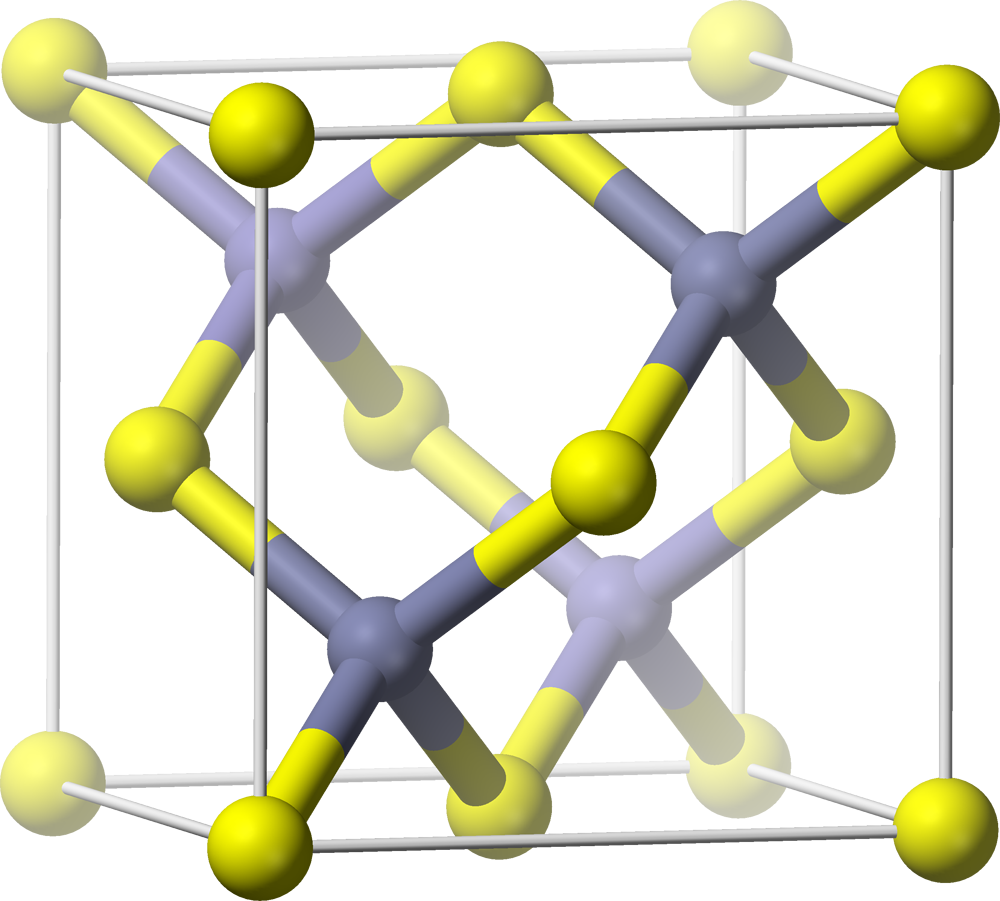
\includegraphics[width=0.6\textwidth]{graphics/zincblende} \\
            \TINY Wikipedia: Zincblende}

            \visible<2->{
            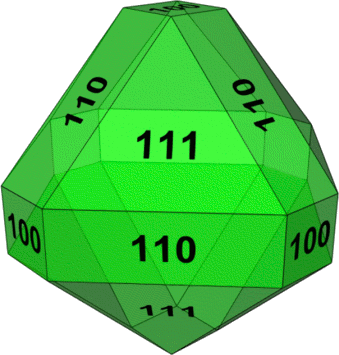
\includegraphics[width=0.6\textwidth]{graphics/symmetry_planes} \\
           \TINY http://www.e6cvd.com/cvd/page.jsp?pageid=361}
           
            \visible<3->{
            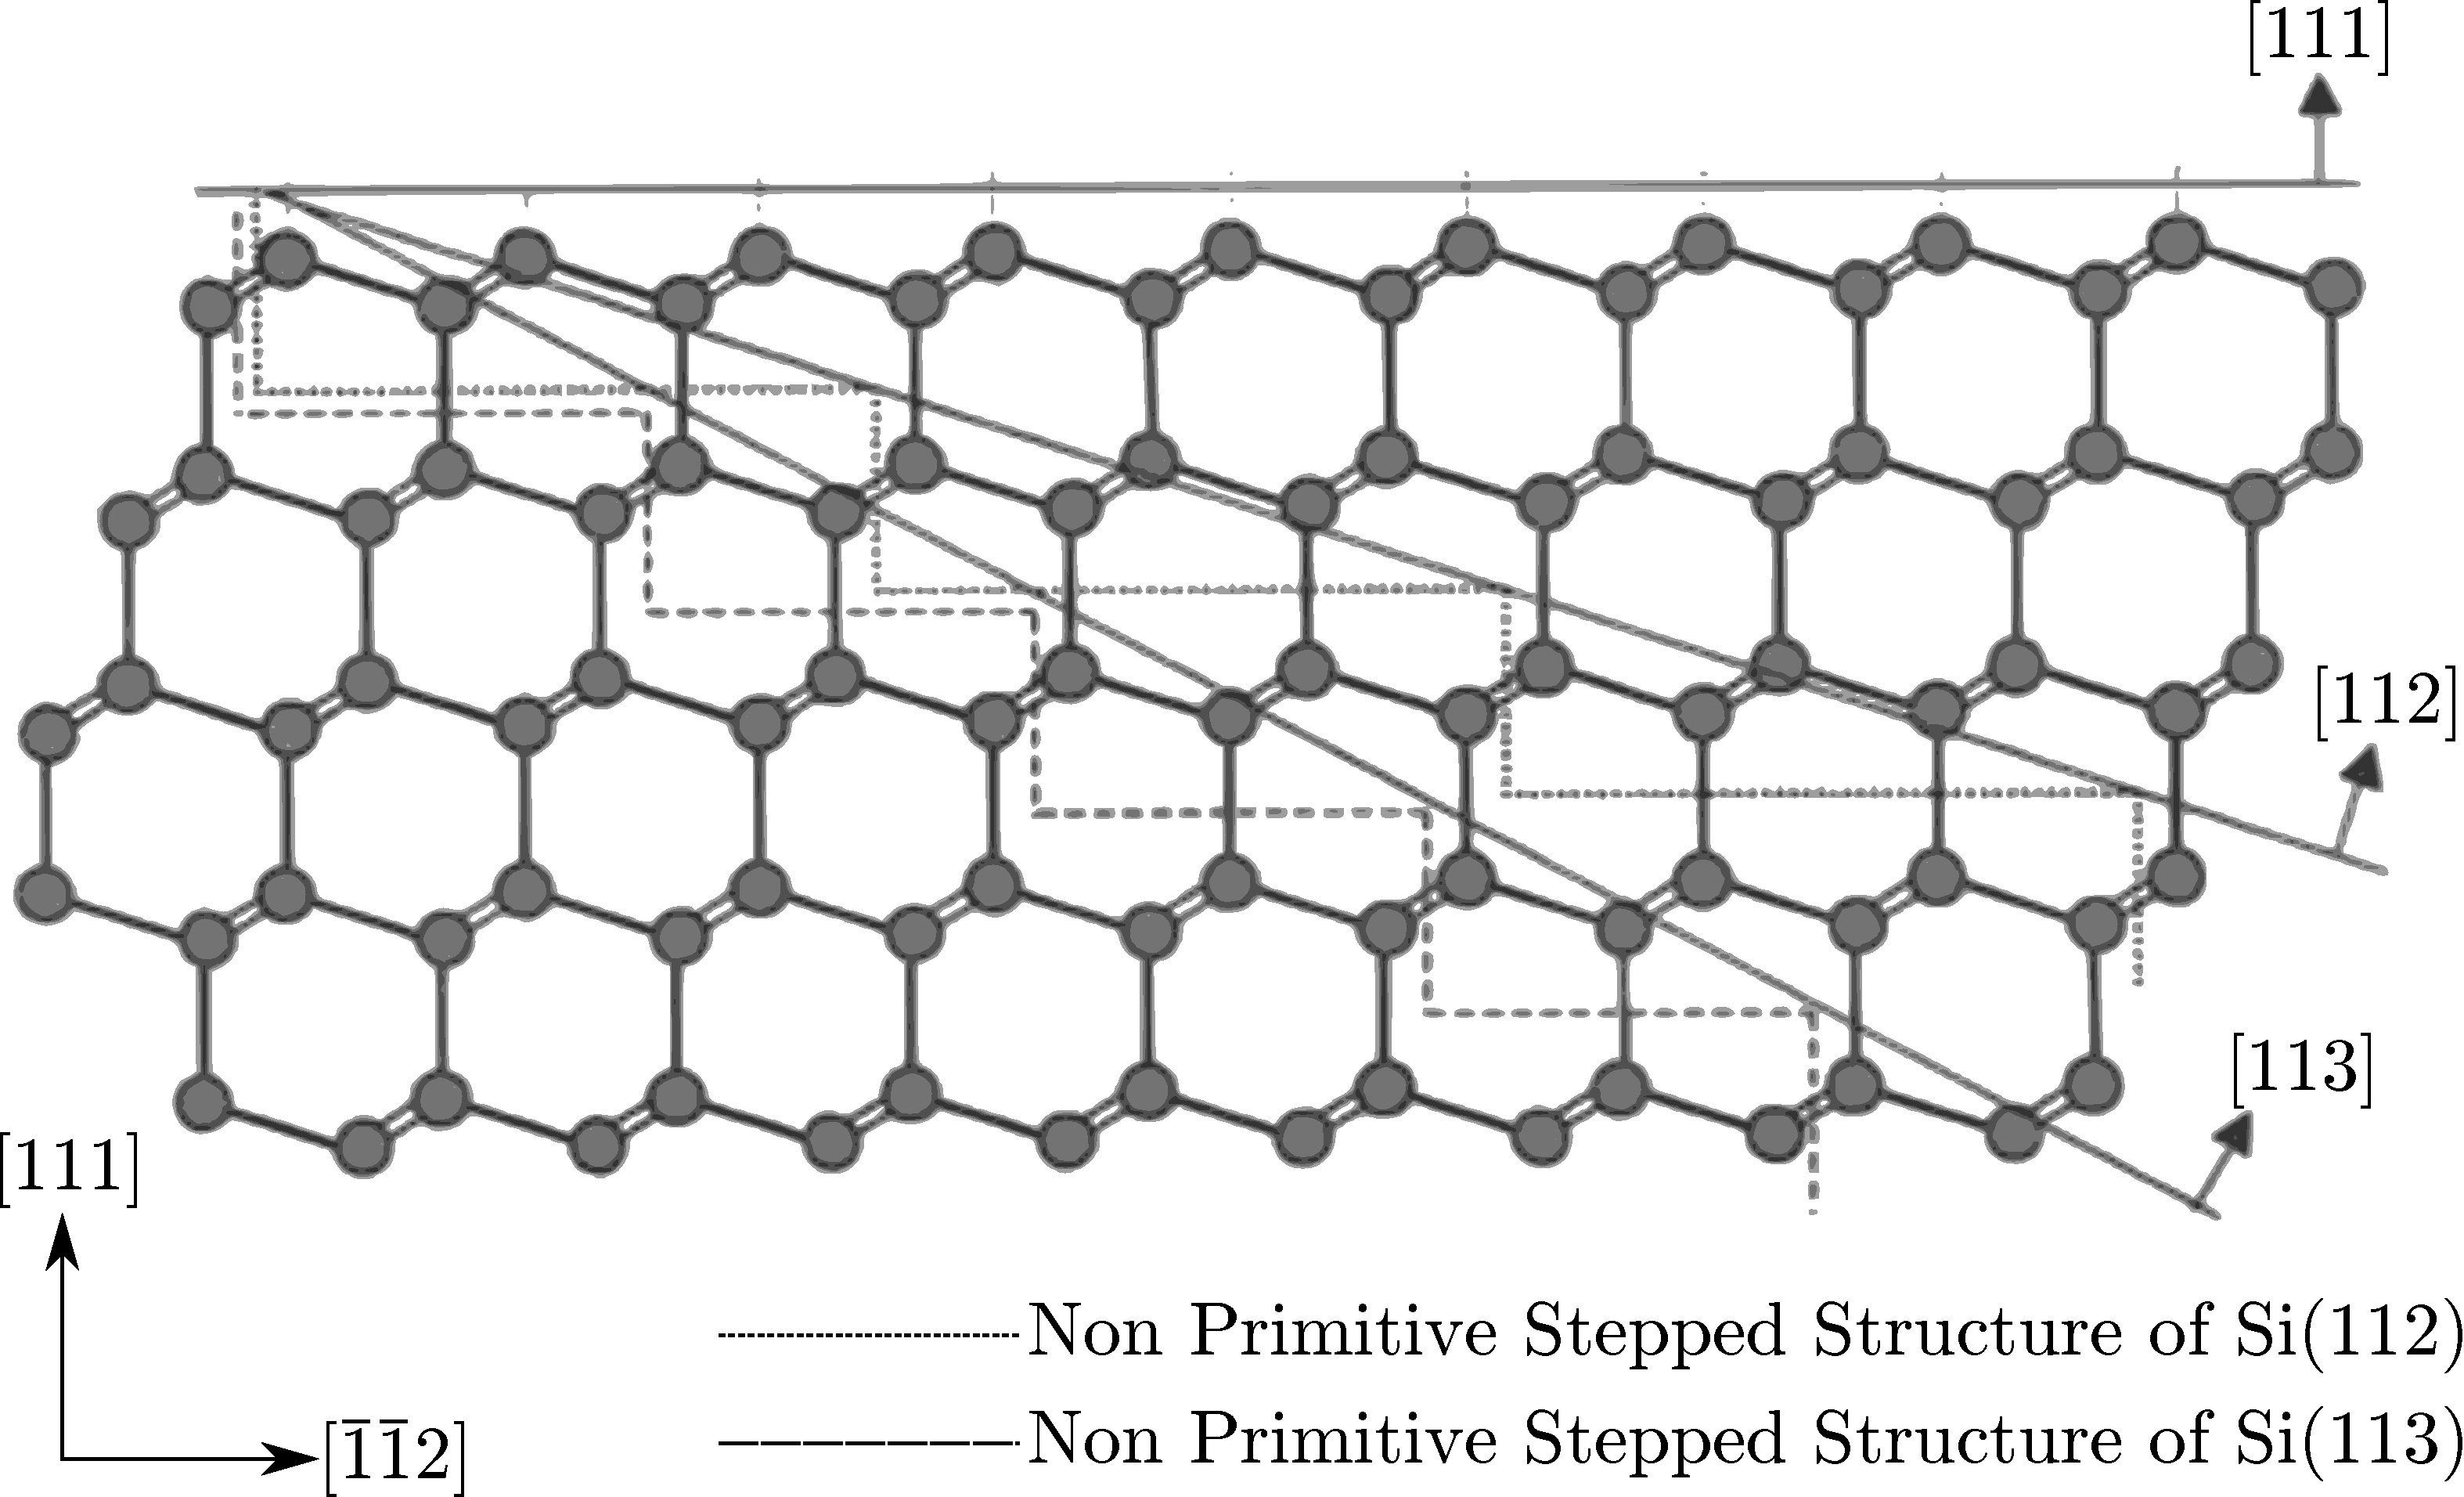
\includegraphics[width=0.95\textwidth]{graphics/211_steps} \\
             \TINY G. Brill, et. al., J. Electron. Mater. 32, 717–722 (2003).}
        \end{column}
        \begin{column}{0.5\textwidth}
            \centering
            \visible<4->{
            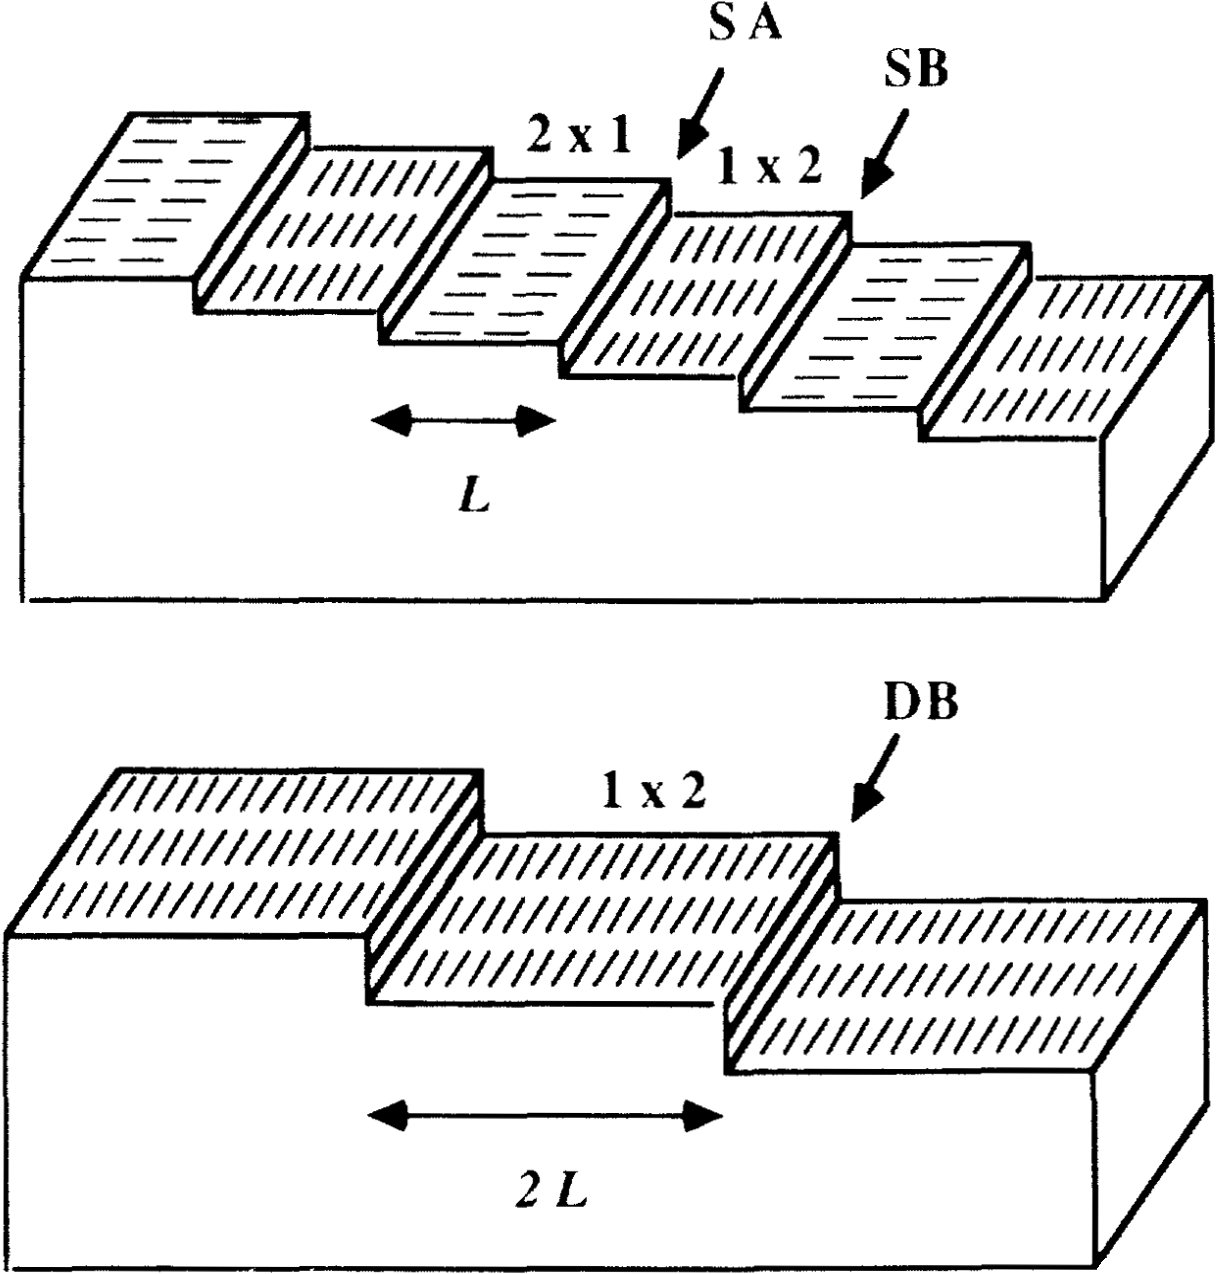
\includegraphics[width=\textwidth]{graphics/back_recon_vicinal} \\
            \TINY O. Alerhand, et. al.,  Phys. Rev. Lett., vol. 64, no. 20, pp. 2406–2409, May 1990.}
            \vspace{0.5cm}
        \end{column}
    \end{columns}
\end{frame}


\subsection{Experimental}
\begin{frame}
        \frametitle{2D X-Ray Diffraction and Pole Figures}
    \begin{columns}[C]
        \begin{column}{0.5\textwidth}
            \centering \visible<1->{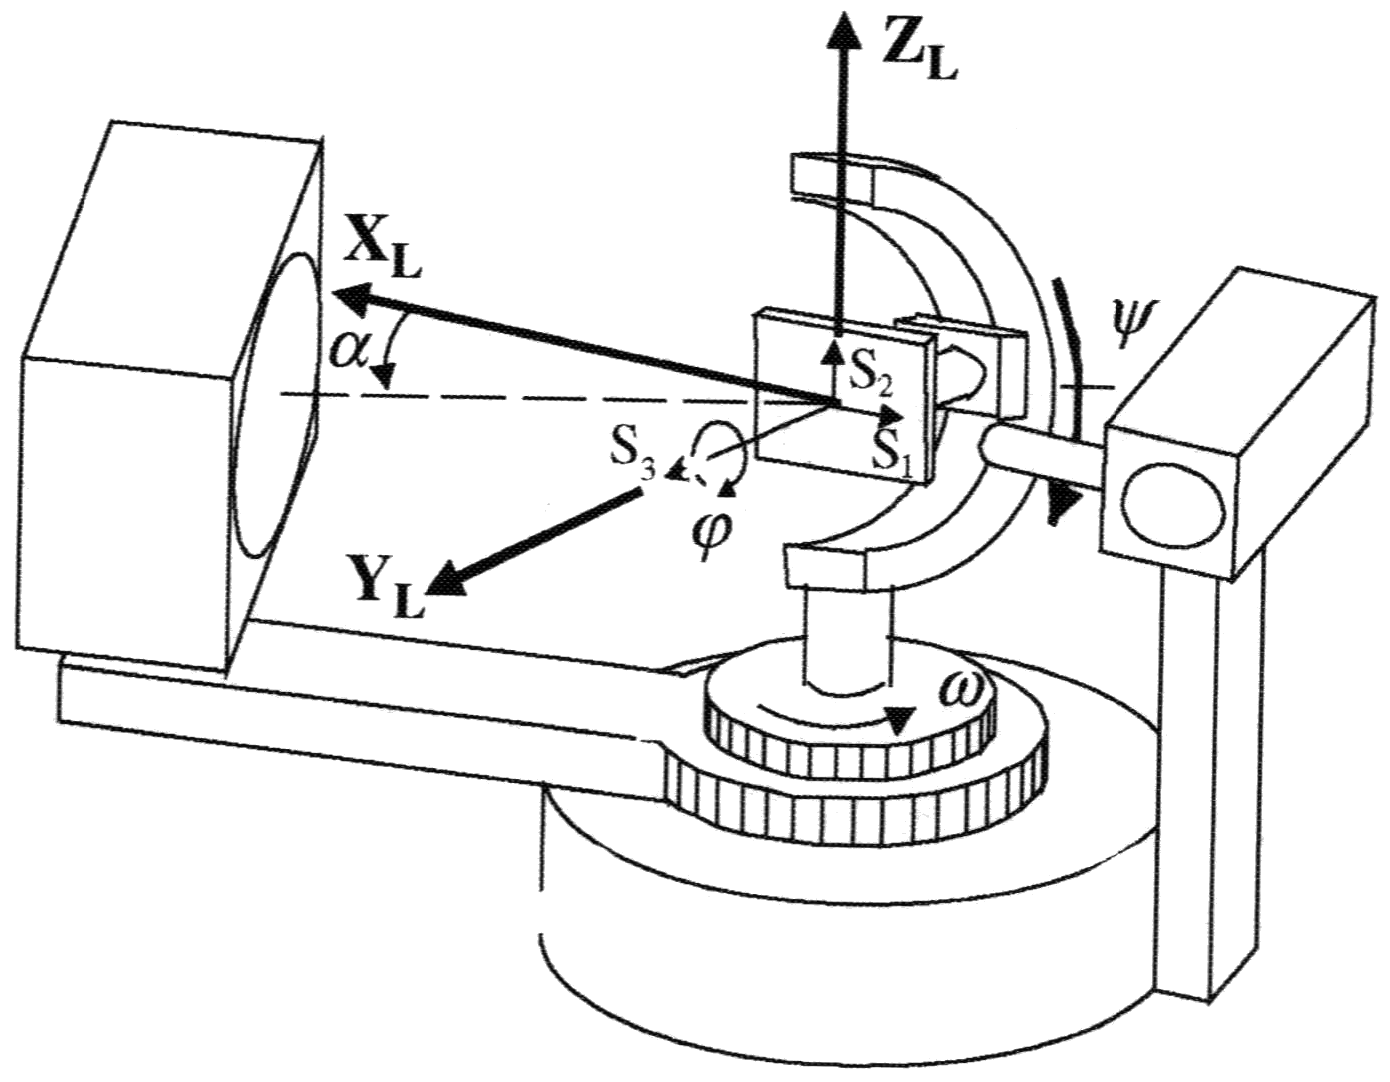
\includegraphics[height=0.43\textheight,keepaspectratio]{graphics/exp_xray_machine}\\ \TINY B. B. He, Two-Dimensional X-Ray Diffraction. Hoboken, NJ, USA: John Wiley \& Sons, Inc., 2009. \\}  \visible<2->{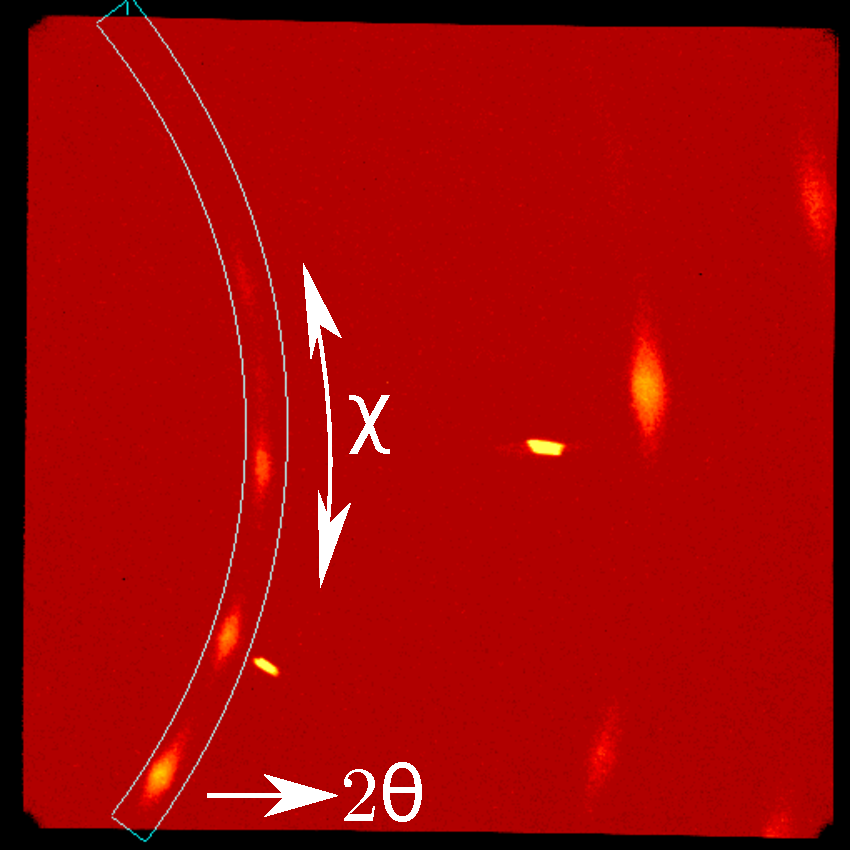
\includegraphics[height=0.46\textheight,keepaspectratio]{graphics/exp_xray_frame}}
        \end{column}
        \begin{column}{0.5\textwidth}
            \centering \visible<3->{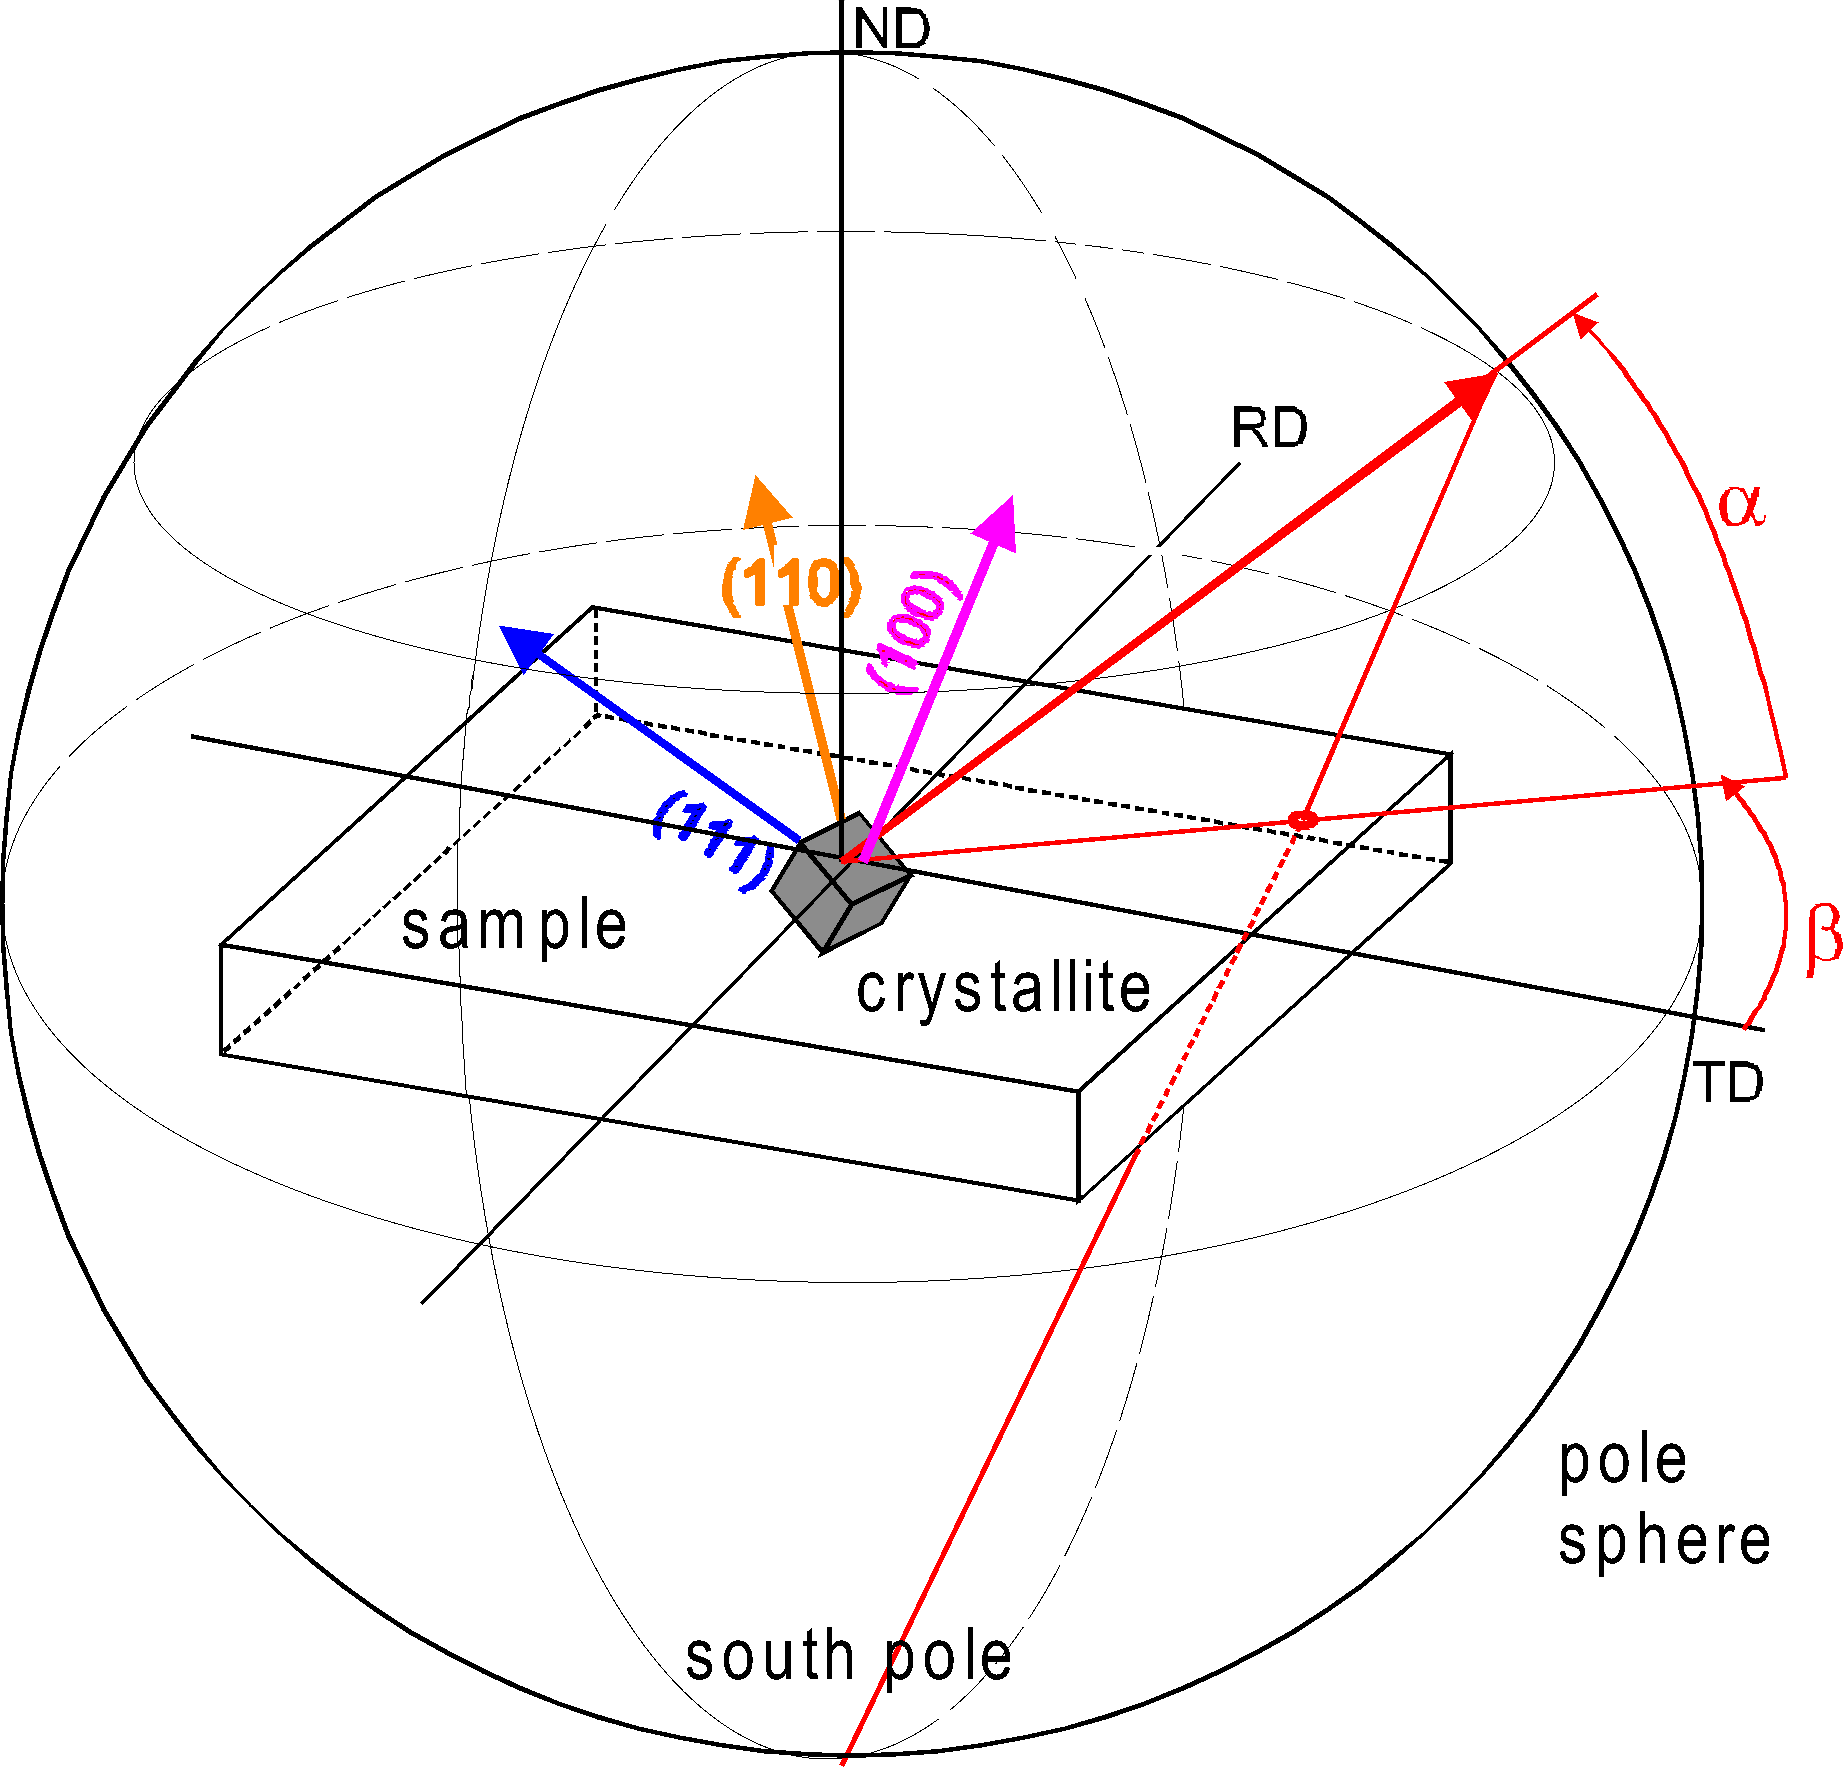
\includegraphics[height=0.43\textheight,keepaspectratio]{graphics/exp_xray_polesphere}\\ \TINY B. B. He, Two-Dimensional X-Ray Diffraction. Hoboken, NJ, USA: John Wiley \& Sons, Inc., 2009.} \\ \visible<4->{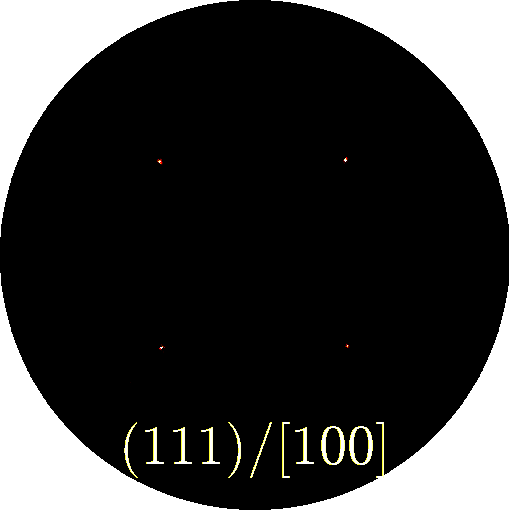
\includegraphics[height=0.44\textheight,keepaspectratio]{graphics/exp_xrd_si_100}}
        \end{column}
    \end{columns}
\end{frame}


\begin{frame}
    \frametitle{Transmission Electron Microscopy}
    \begin{columns}
        \begin{column}{0.5\textwidth}
               \centering
               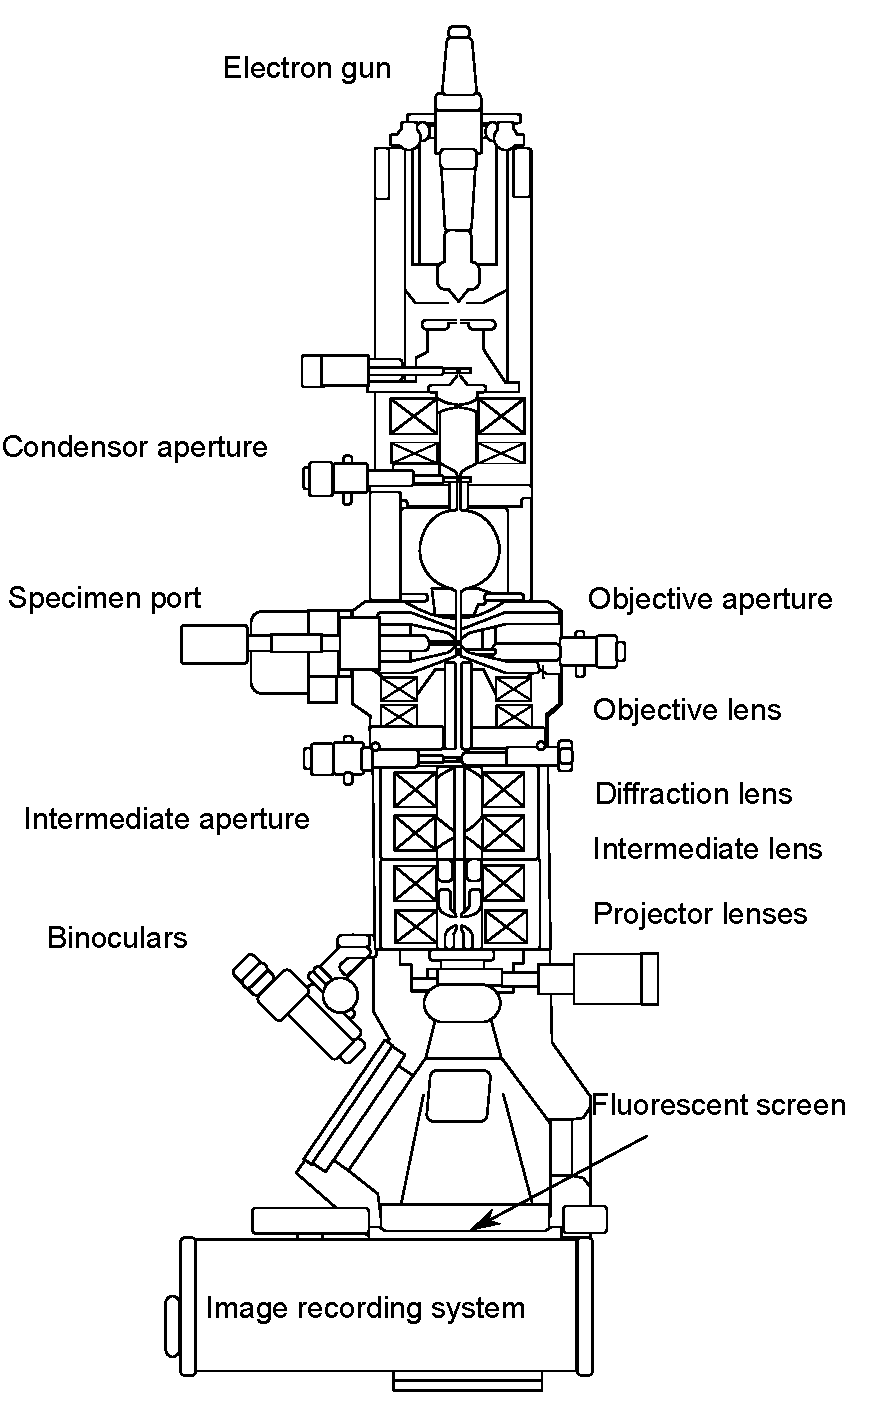
\includegraphics[width=\textwidth,height=0.85\textheight,keepaspectratio]{graphics/TEM} \\
               \TINY Wikipedia: TEM
        \end{column}
        \begin{column}{0.5\textwidth}
            \only<1>{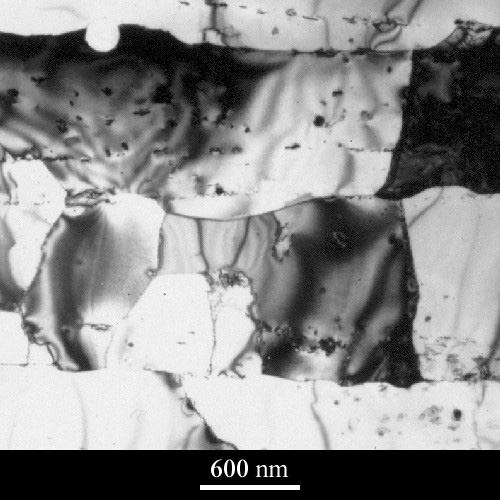
\includegraphics[width=\textwidth]{graphics/tem_example} \\ \TINY DoITPoMS: 608}
            \only<2>{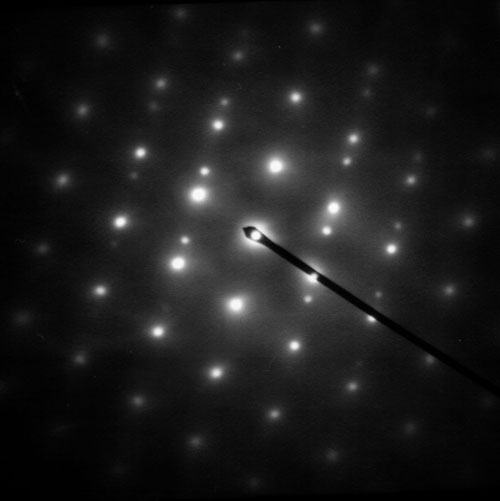
\includegraphics[width=\textwidth]{graphics/tem_diffraction} \\ \TINY Wikipedia: TEM}
        \end{column}
    \end{columns}
\end{frame}


\begin{frame}
        \frametitle{Growth}
    \begin{columns}
        \begin{column}{0.54\textwidth}
            \centering
            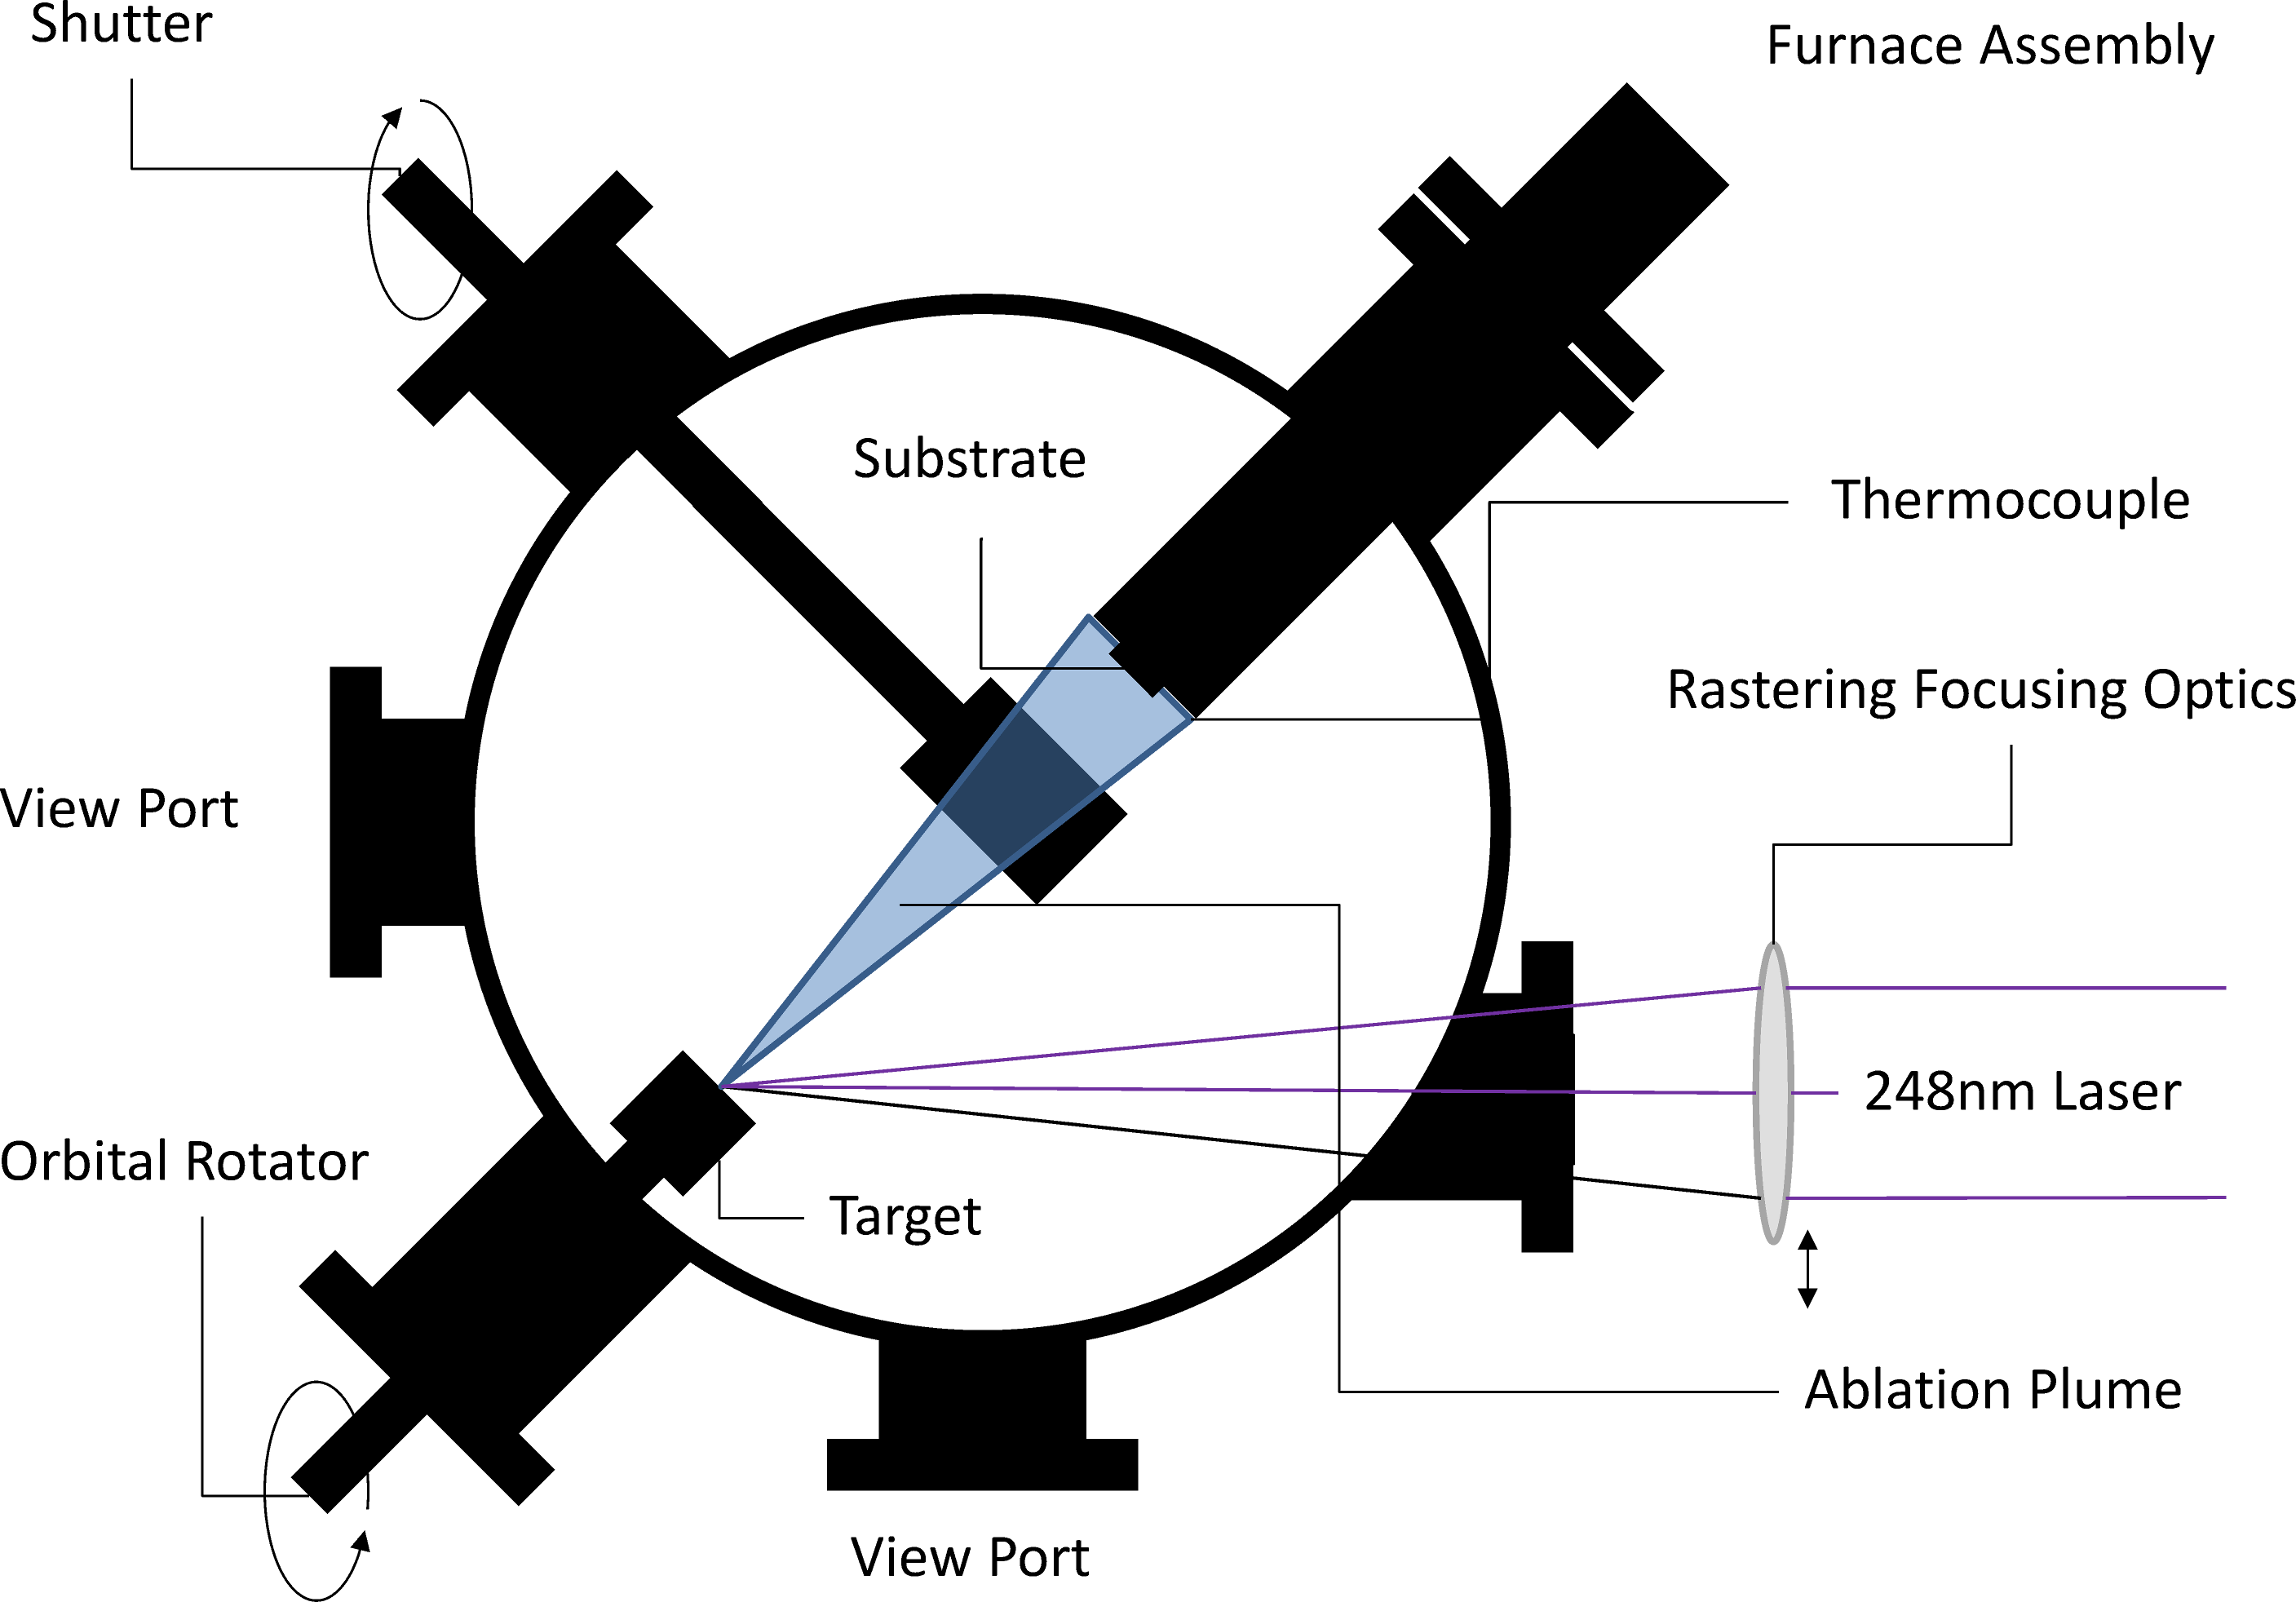
\includegraphics[width=\textwidth]{graphics/exp_PLD_chamber} \\
            Pulsed Laser Deposition (PLD)
        \end{column}
        \begin{column}{0.46\textwidth}
            \centering
           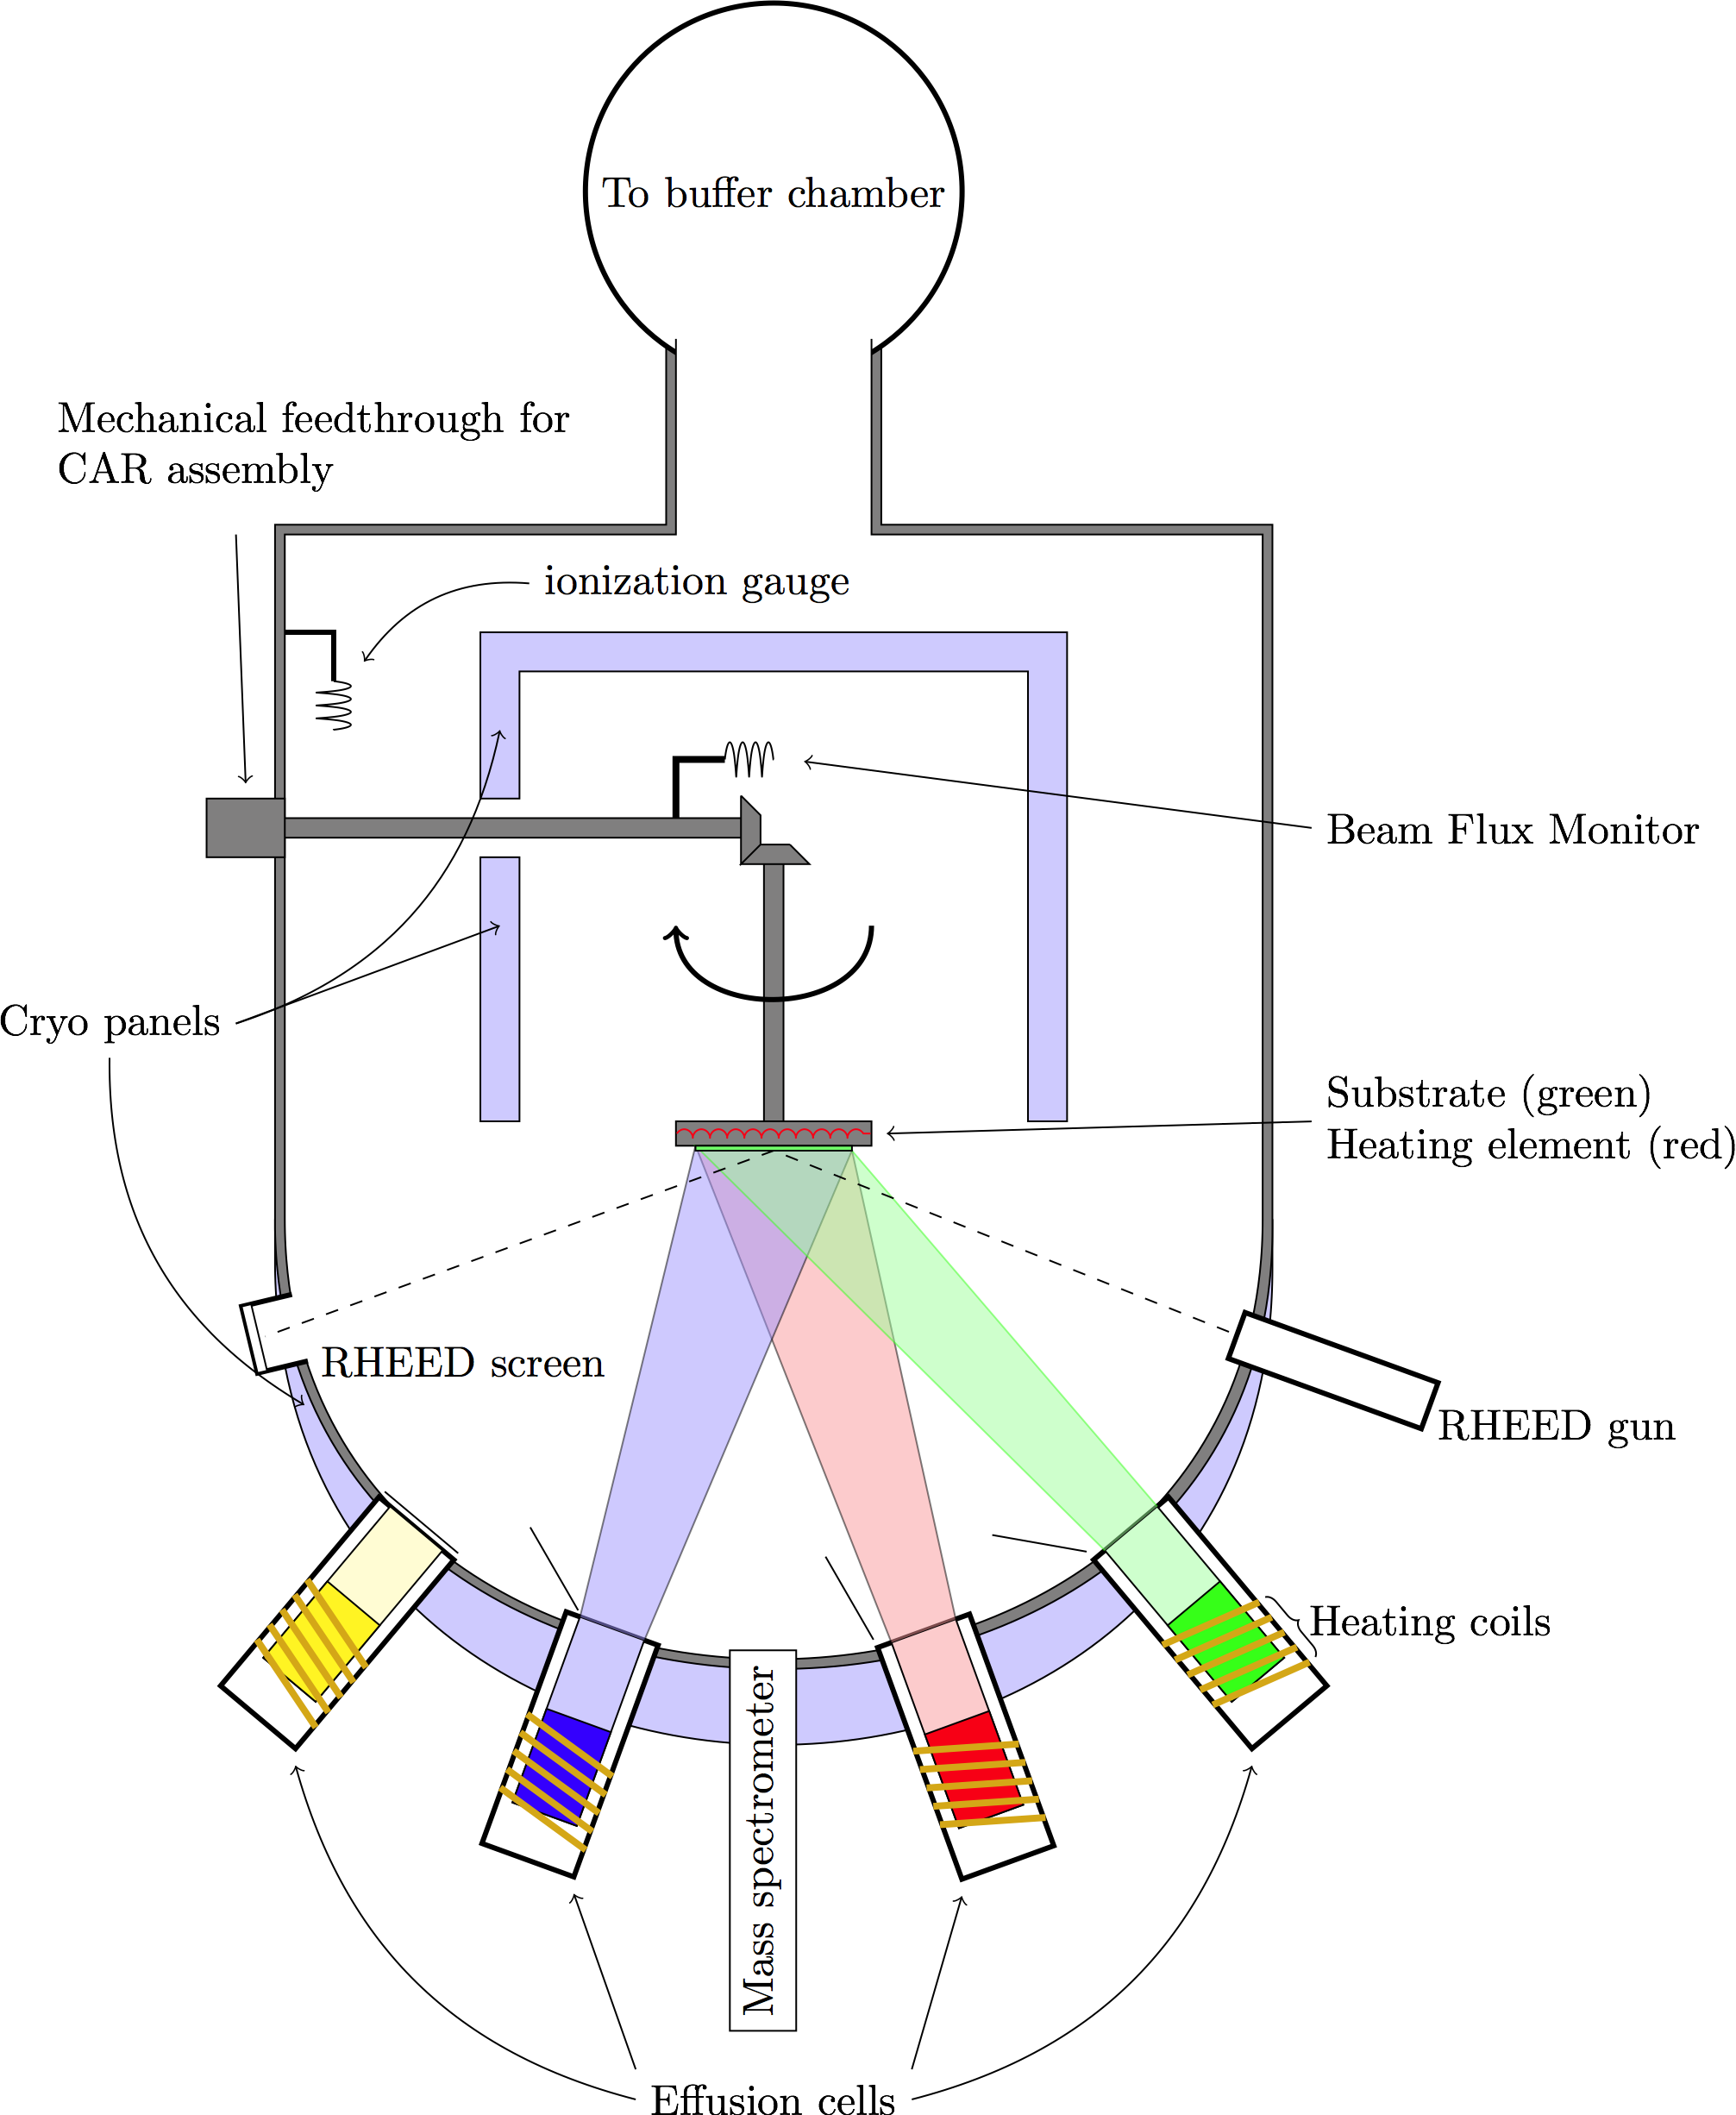
\includegraphics[width=0.95\textwidth]{graphics/MBE} \\
           Molecular Beam Epitaxy (MBE) \\
           \TINY Wikipedia: MBE
        \end{column}
    \end{columns}
\end{frame}

\section{Symmetry Breaking at Interfaces}
\subsection{Twins and Epitaxy on Vicinal (Offcut) (001) Silicon}
\begin{frame}
\frametitle{Outline}
 \tableofcontents[currentsection,currentsubsection]
\end{frame}

\begin{frame}
    \frametitle{Twins and Epitaxy on Vicinal (001) Silicon}
    \begin{columns}
        \begin{column}{0.5\textwidth}
            \begin{block}{Introduction}
                \begin{itemize}[<+-| alert@+>]
                    \item Semiconductors are most commonly the zincblende crystal structure
                    \item Twins (stacking faults on <111> planes) are common low energy defects
                    \item Investigations into III-V epitaxy showed a relationship between vicinal (offcut) substrates and twinning
                \end{itemize}
            \end{block}
        \end{column}
        \begin{column}{0.5\textwidth}
            \centering
            \visible<1->{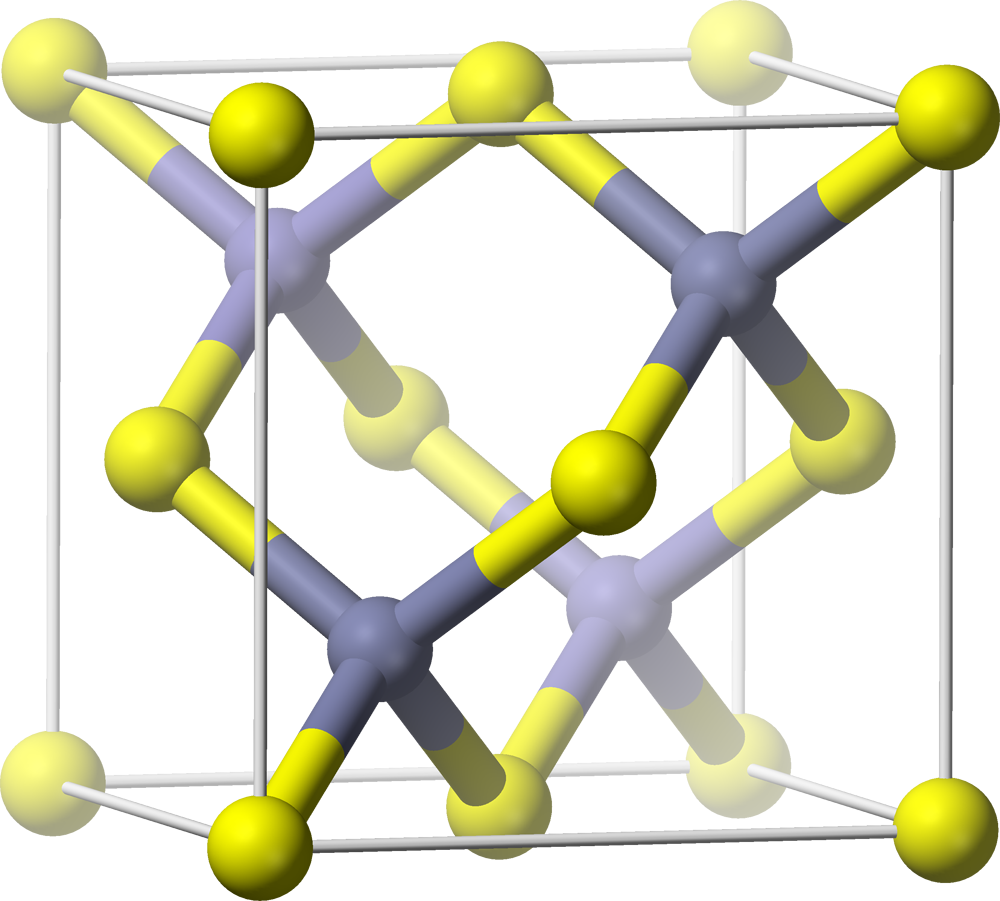
\includegraphics[height=0.4\textheight]{graphics/zincblende} \\ \TINY Wikipedia: Zincblende} \\
            \visible<2->{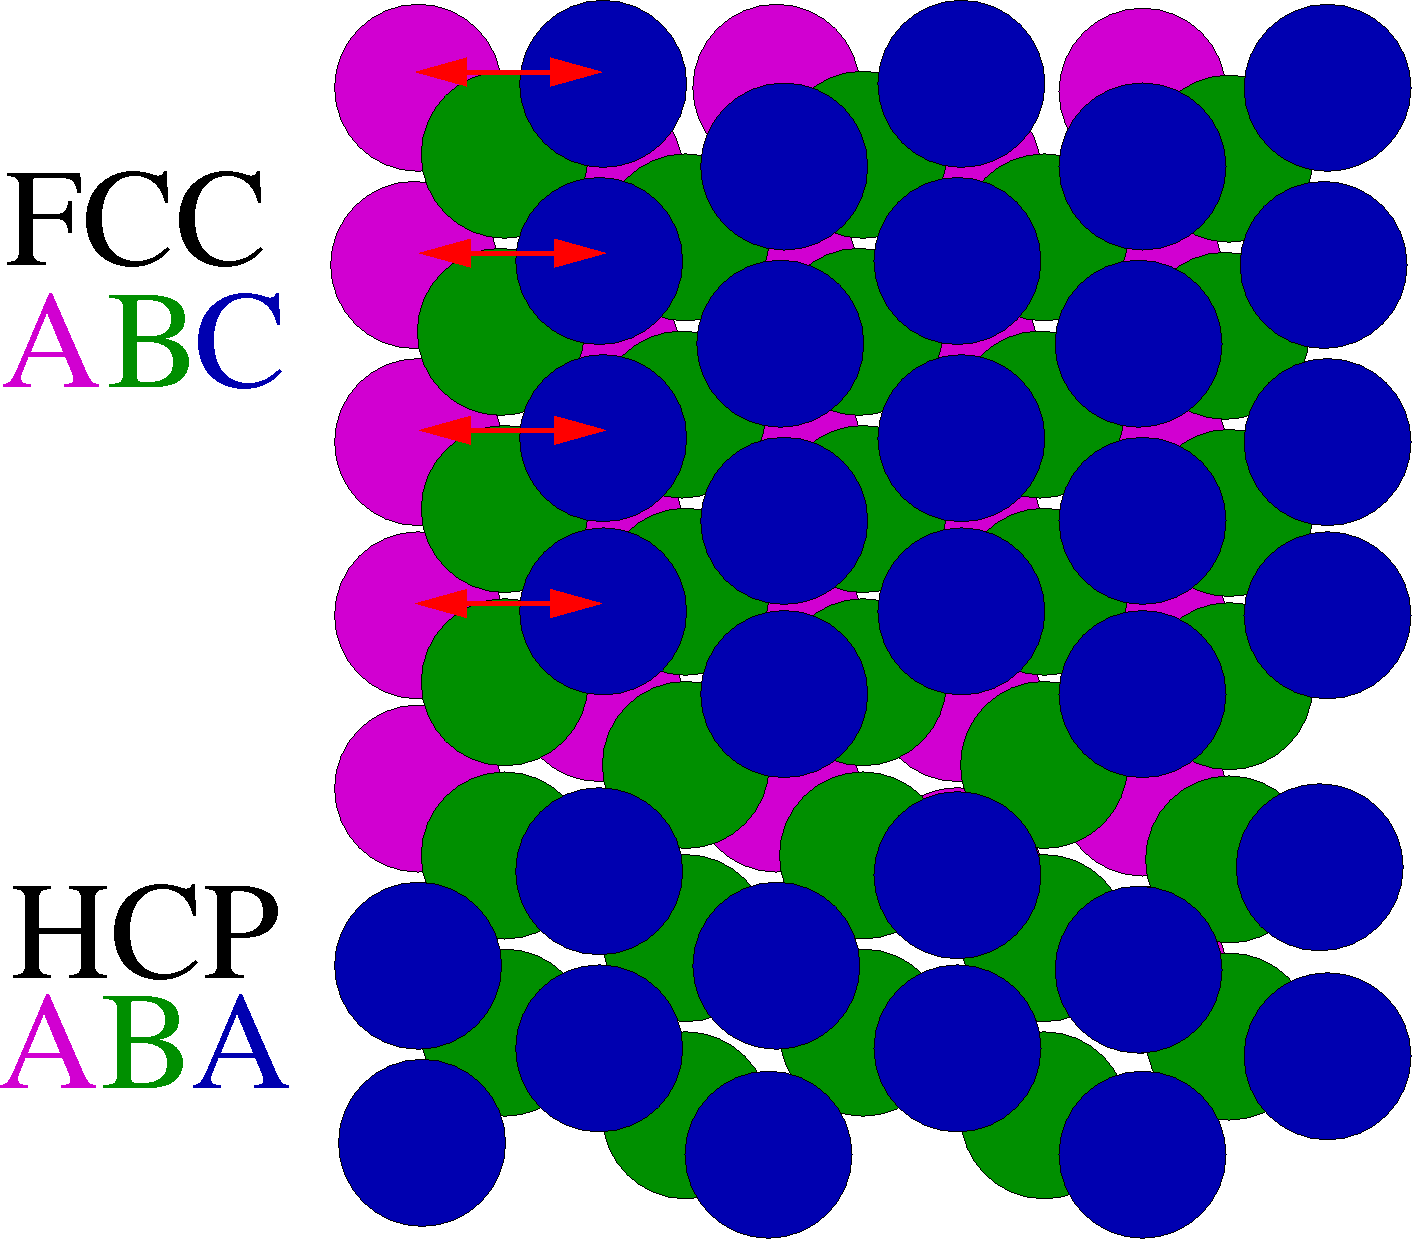
\includegraphics[height=0.4\textheight]{graphics/stacking_fault}\\ \TINY Wikipedia: Crystallographic defect}
        \end{column}
    \end{columns}
\end{frame}

\begin{frame}
    \frametitle{Twins and Epitaxy on Vicinal (001) Silicon}
        \begin{columns}
            \begin{column}{0.5\textwidth}
                \begin{block}{Experiemental}
                    \begin{itemize}[<+-| alert@+>]
                        \item Nominal (flat) and vicinal (offcut) silicon (001) substrates
                        \item Initially investigated due to their ability to control anti-phase boundaries in III-V epitaxy via step formation
                        \item Substrates were reconstructed \textit{in-situ} in the MBE via thermal treatment
                        \item 500~nm films of GaAs, InP, GaSb, and AlSb were deposited, covering a lattice mismatch of 4--13\%
                    \end{itemize}
                \end{block}
            \end{column}
            \begin{column}{0.5\textwidth}
                \centering
                \only<1-2>{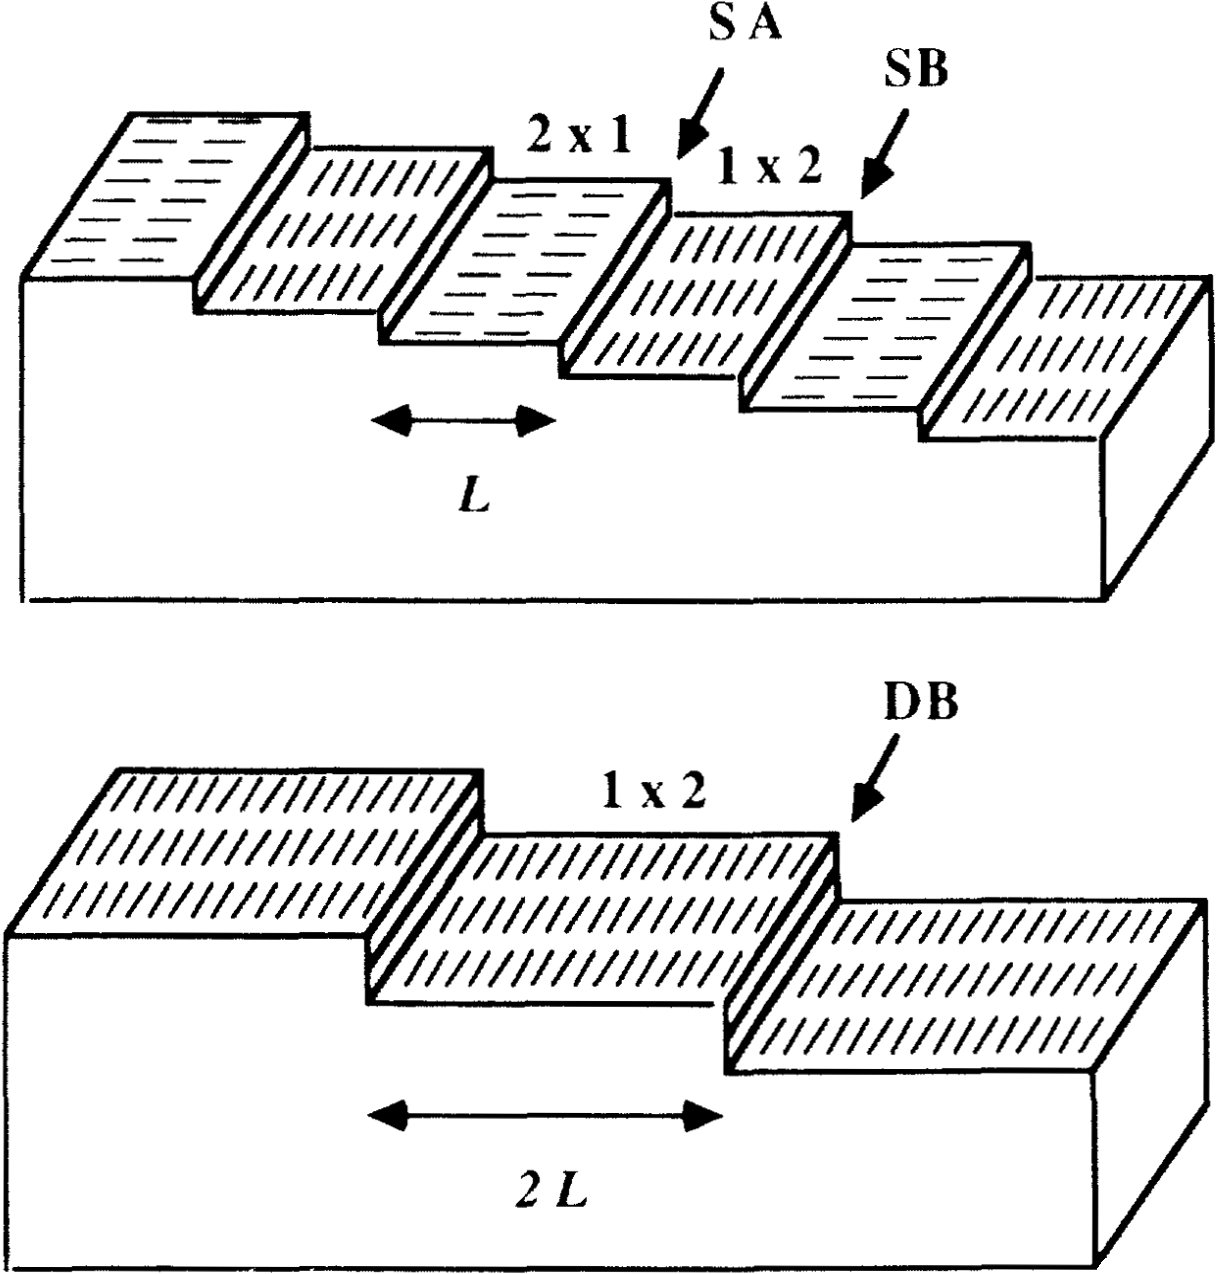
\includegraphics[height=0.9\textheight,width=\textwidth,keepaspectratio]{graphics/back_recon_vicinal}\\ \TINY O. Alerhand, et. al.,  Phys. Rev. Lett., vol. 64, no. 20, pp. 2406–2409, May 1990.} \\
                \only<3->{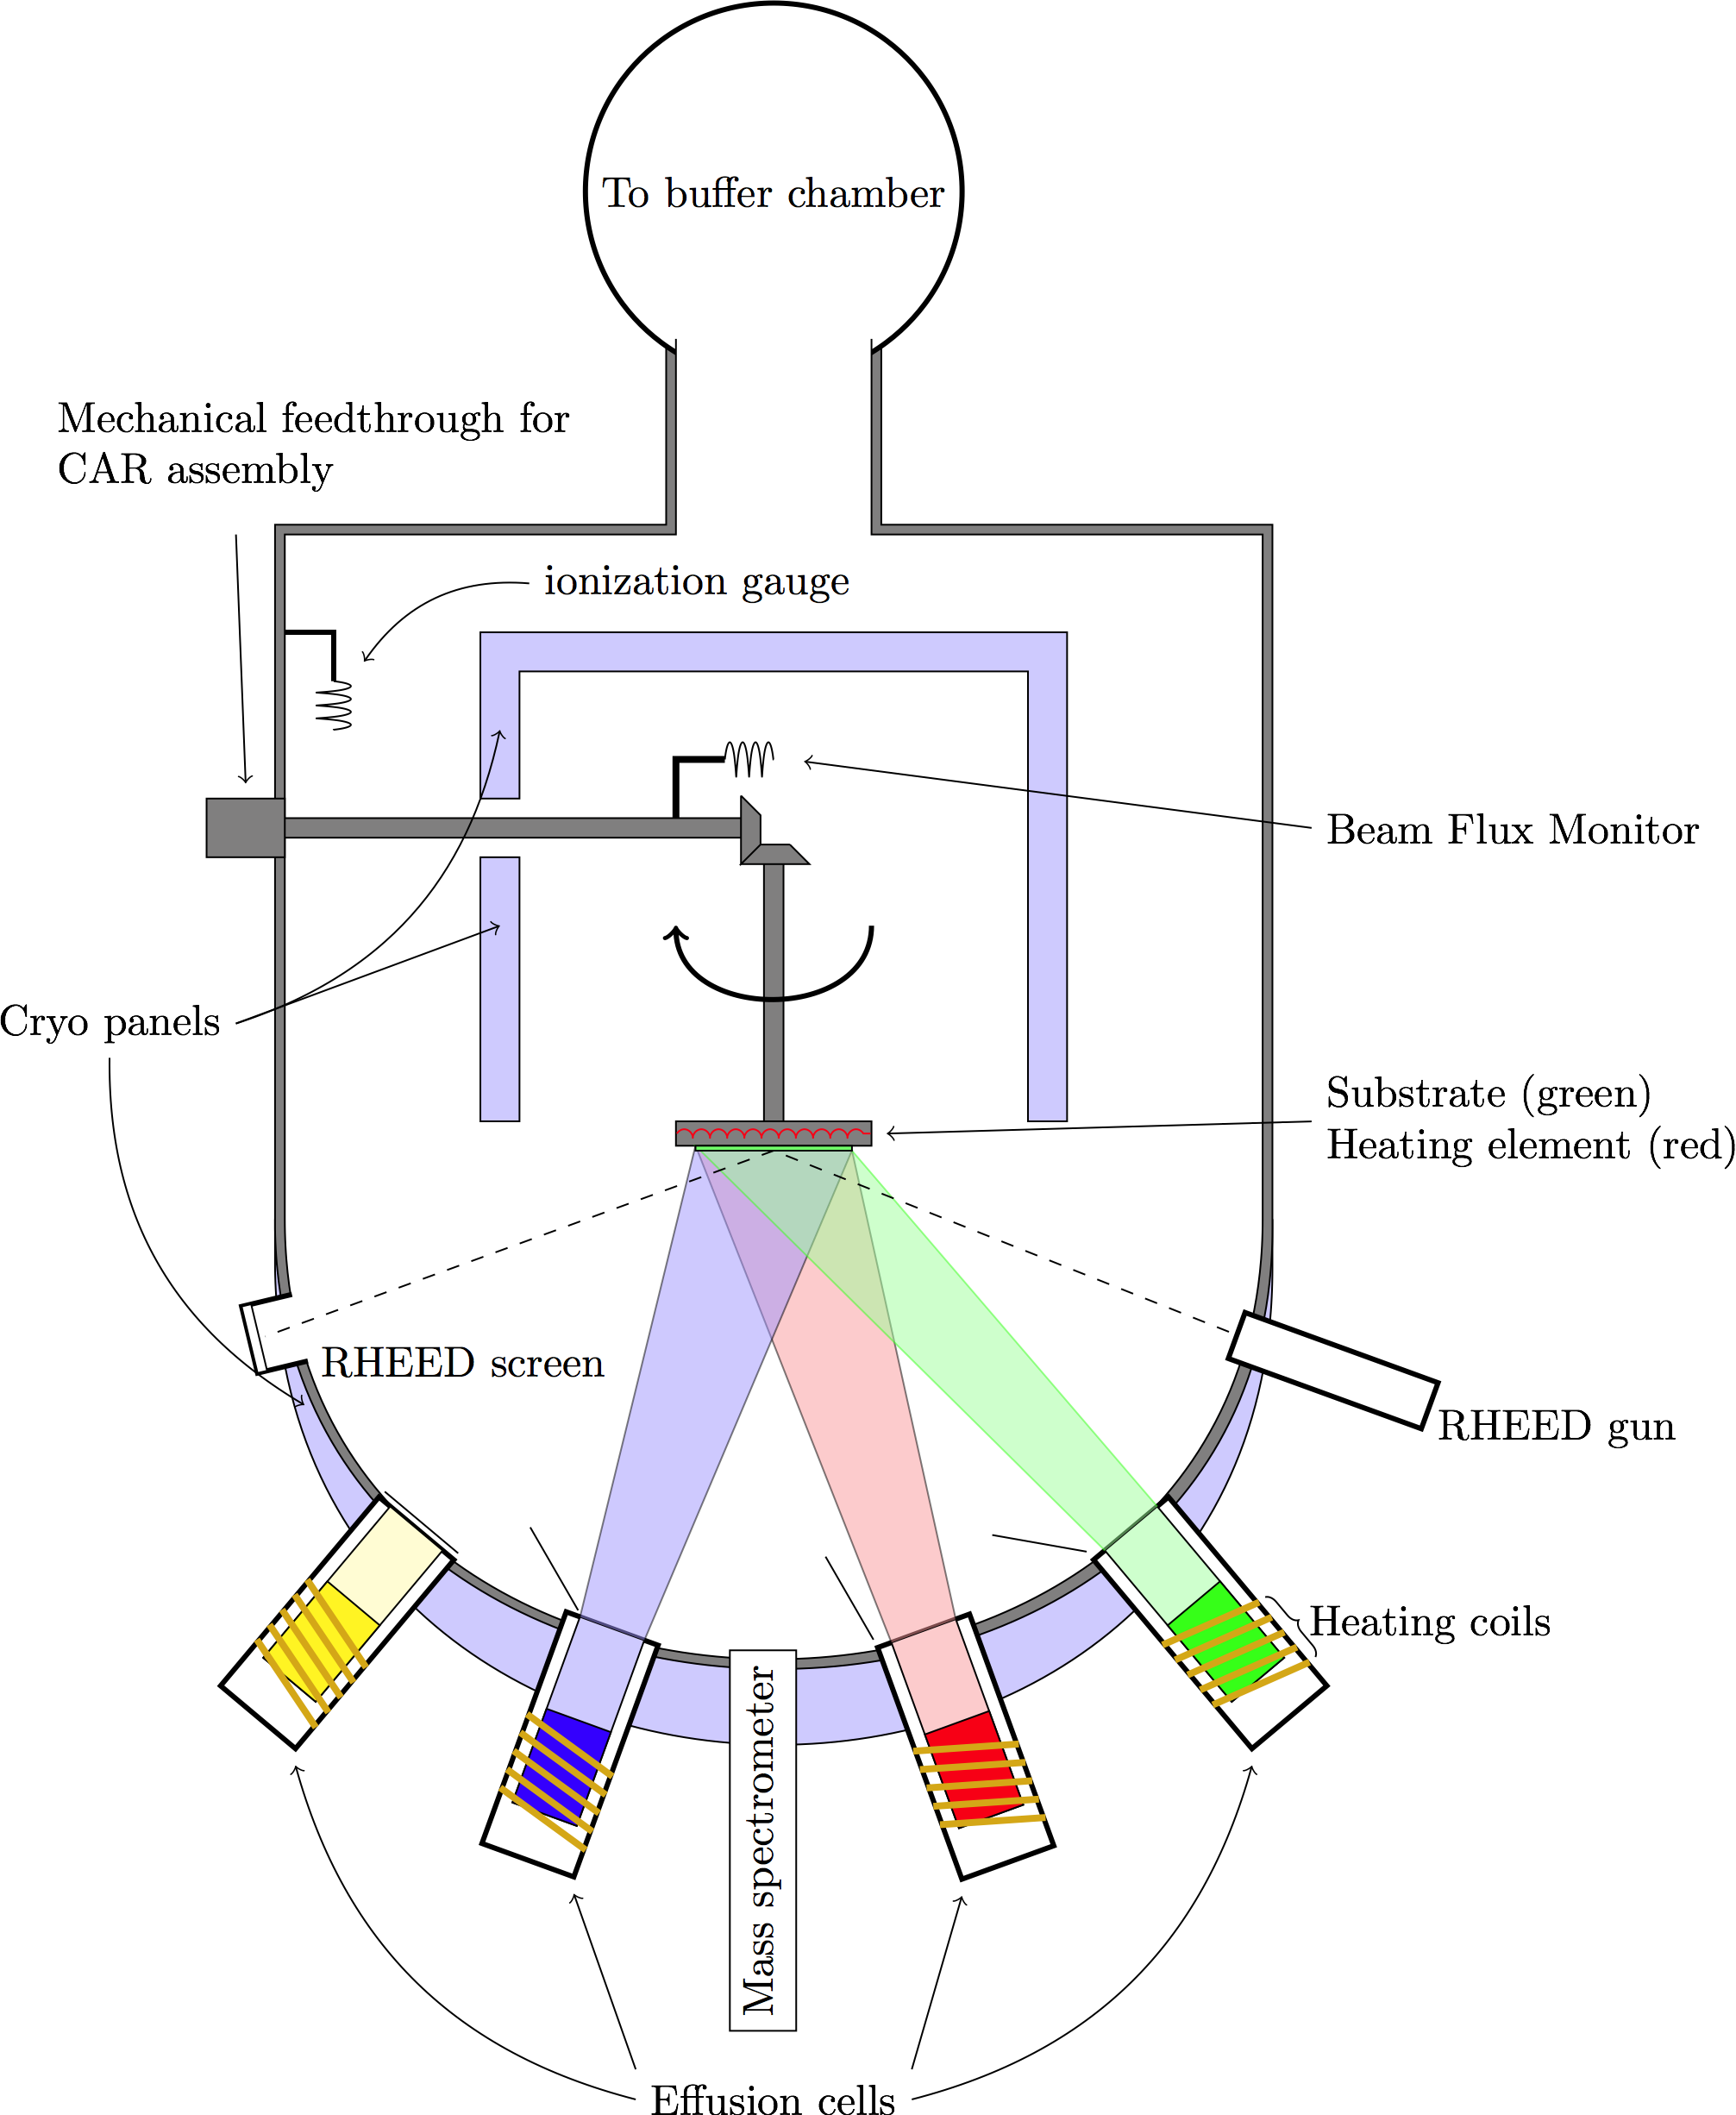
\includegraphics[height=0.9\textheight,width=\textwidth,keepaspectratio]{graphics/MBE} \\ \TINY Wikipedia: MBE}
            \end{column}
        \end{columns}
\end{frame}

\begin{frame}
    \frametitle{(111) 2DXRD Pole Figures}
    \begin{center}
        \only<1>{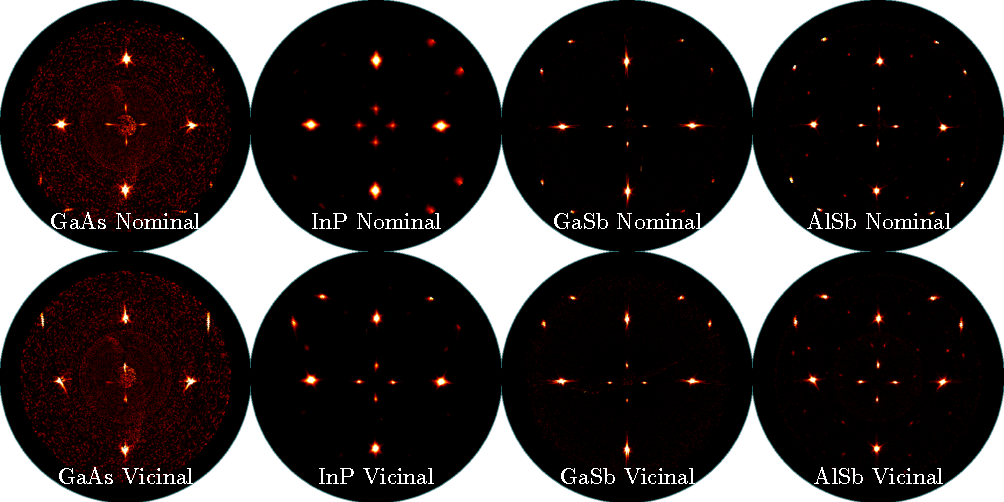
\includegraphics[width=\textwidth]{graphics/twins_polefigure}}
        \only<2>{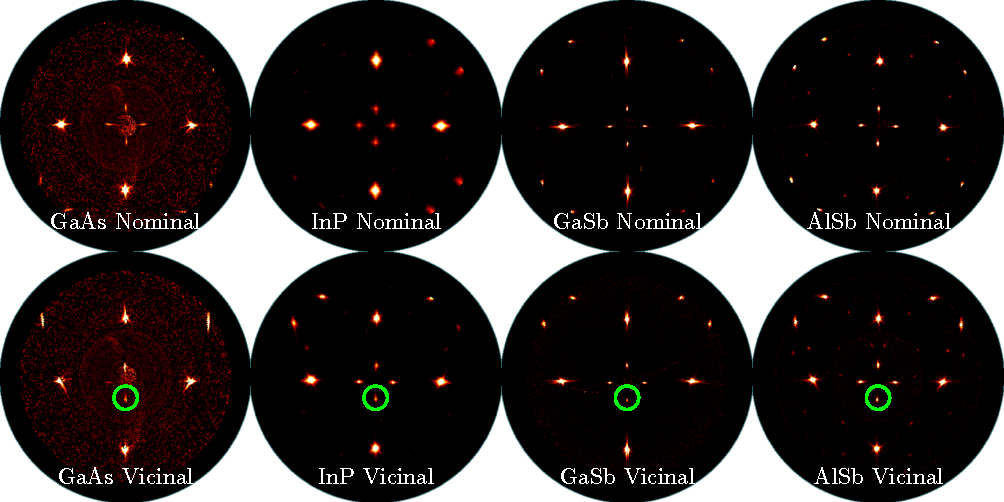
\includegraphics[width=\textwidth]{graphics/twins_polefigure_highlight}}
    \end{center}
\end{frame}

%TODO Fix up TEM labelles and step direction
\begin{frame}
    \frametitle{(111) Pole Figure Modelling and Intensity}
    \begin{columns}
        \begin{column}{0.5\textwidth}
            \begin{figure}
                \only<1-2>{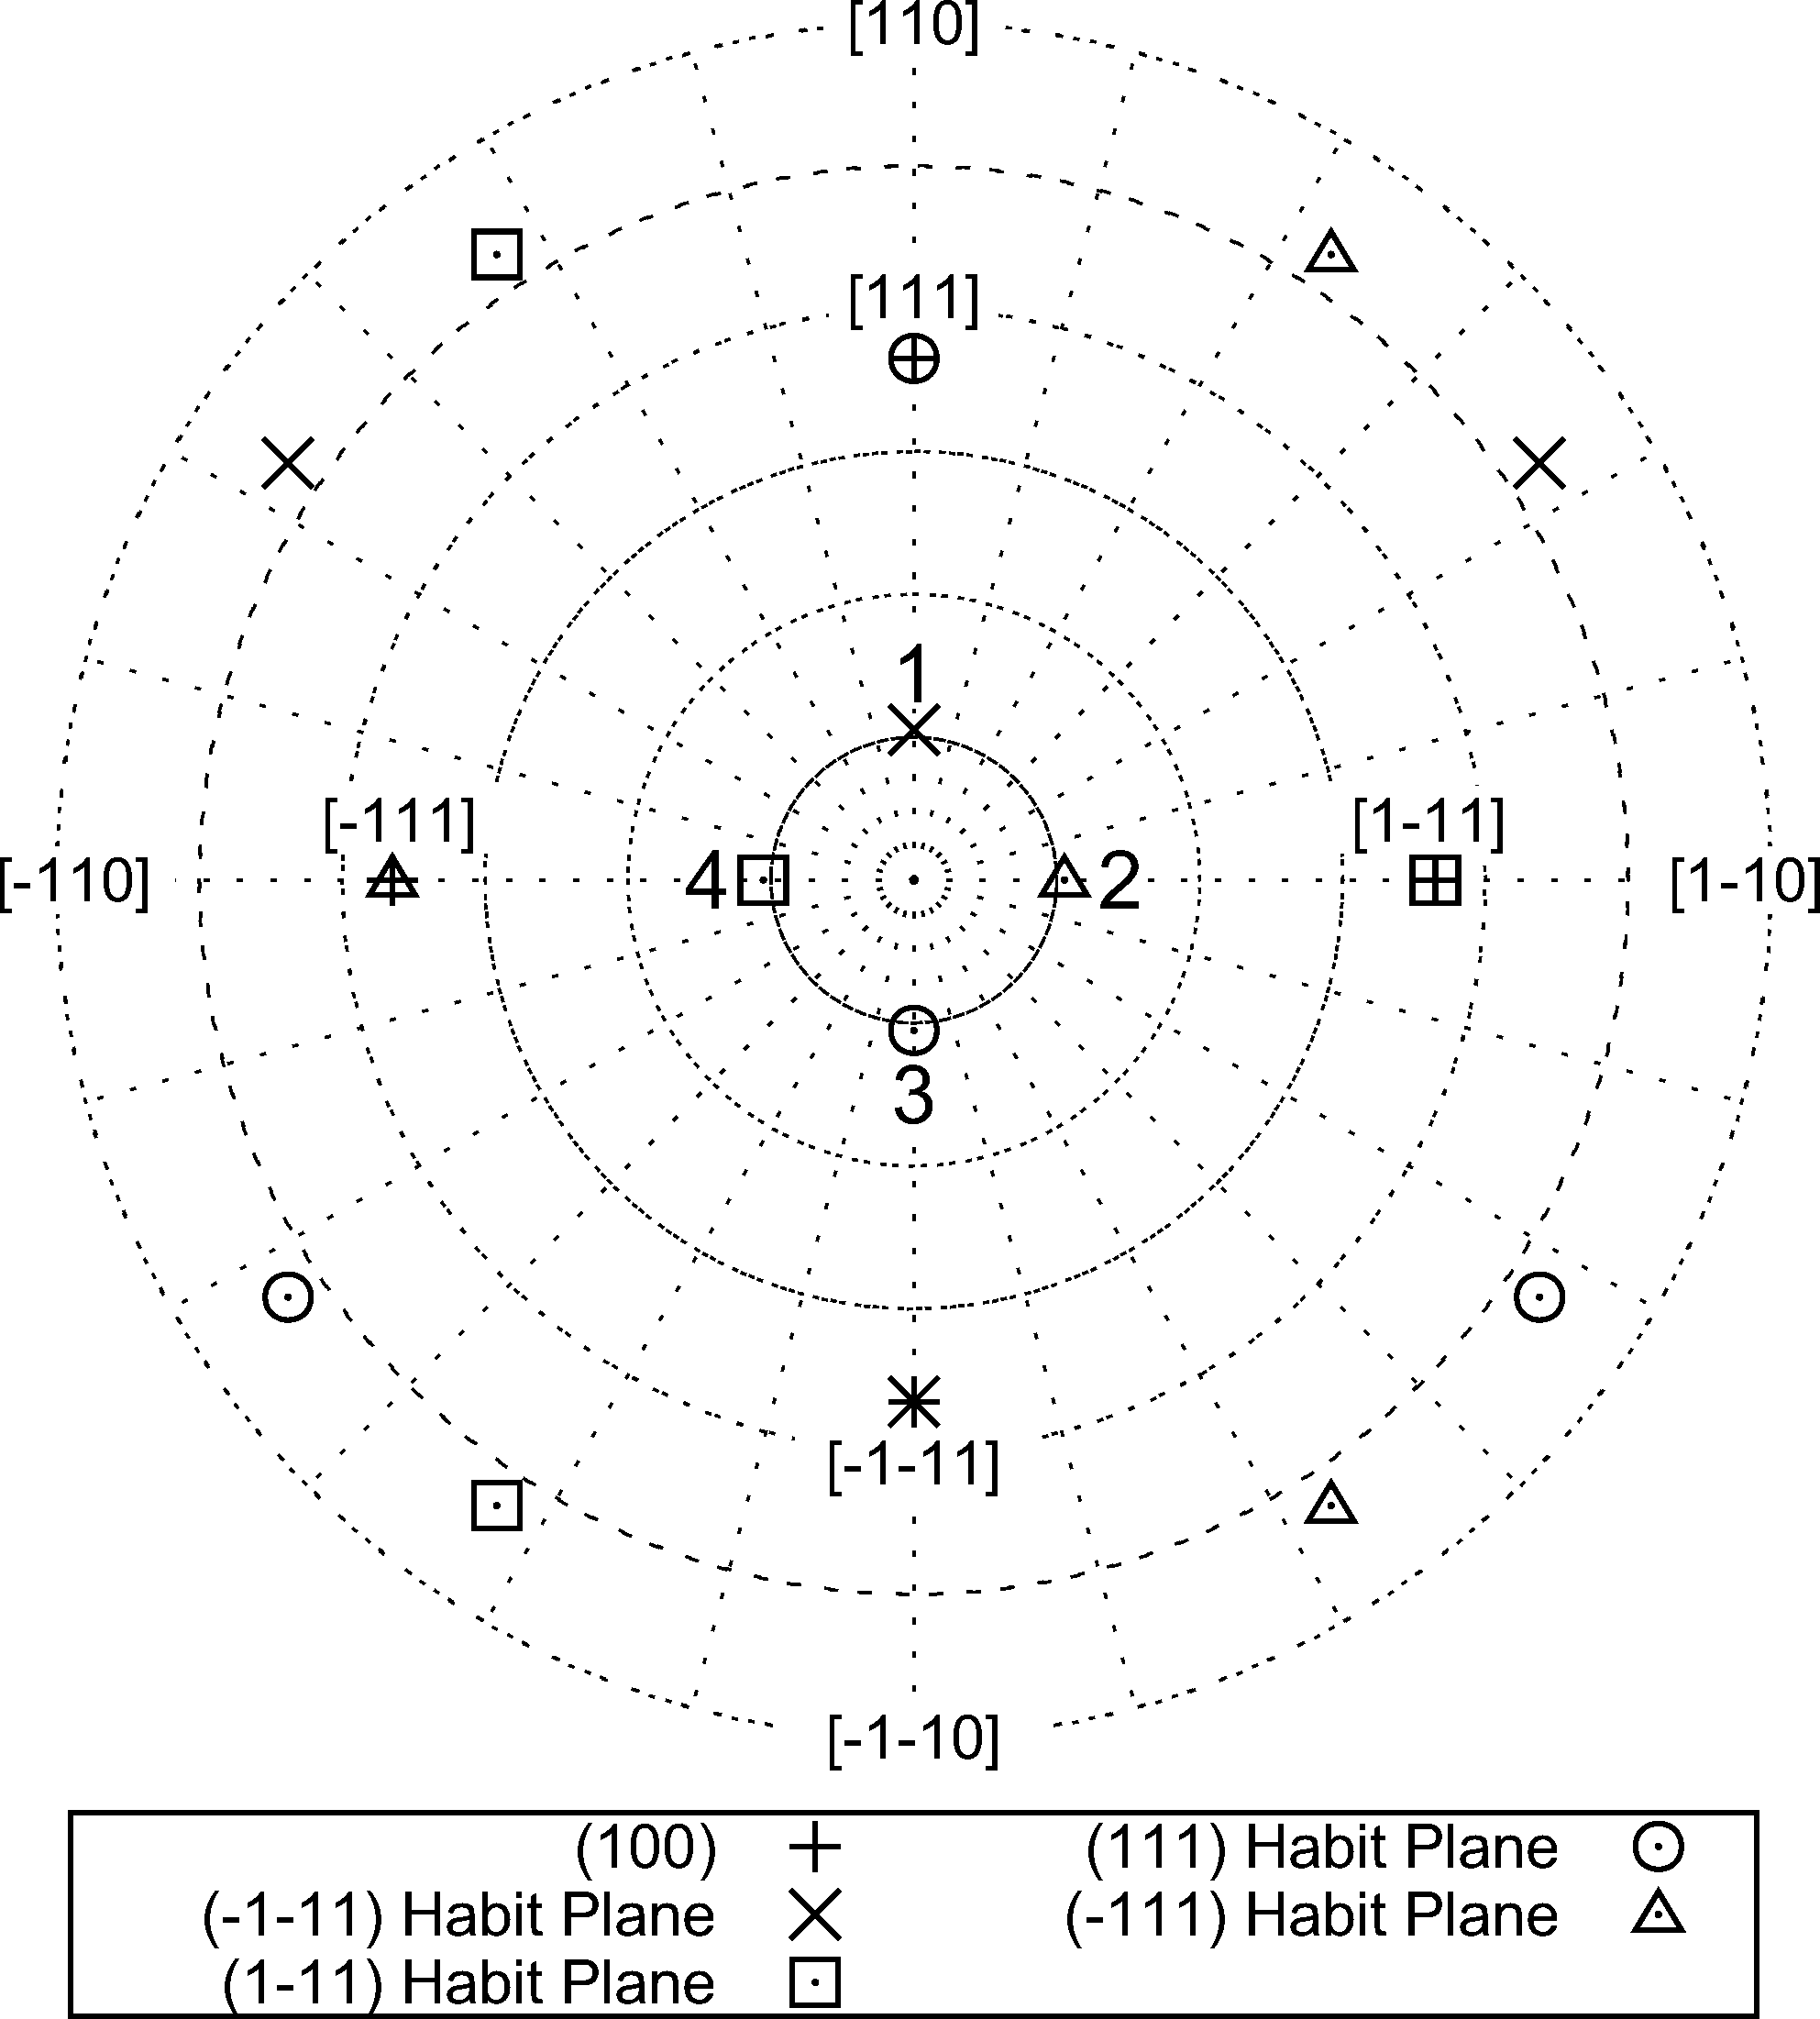
\includegraphics[width=\textwidth]{graphics/twins_simulated_polefigure}}
                \only<3>{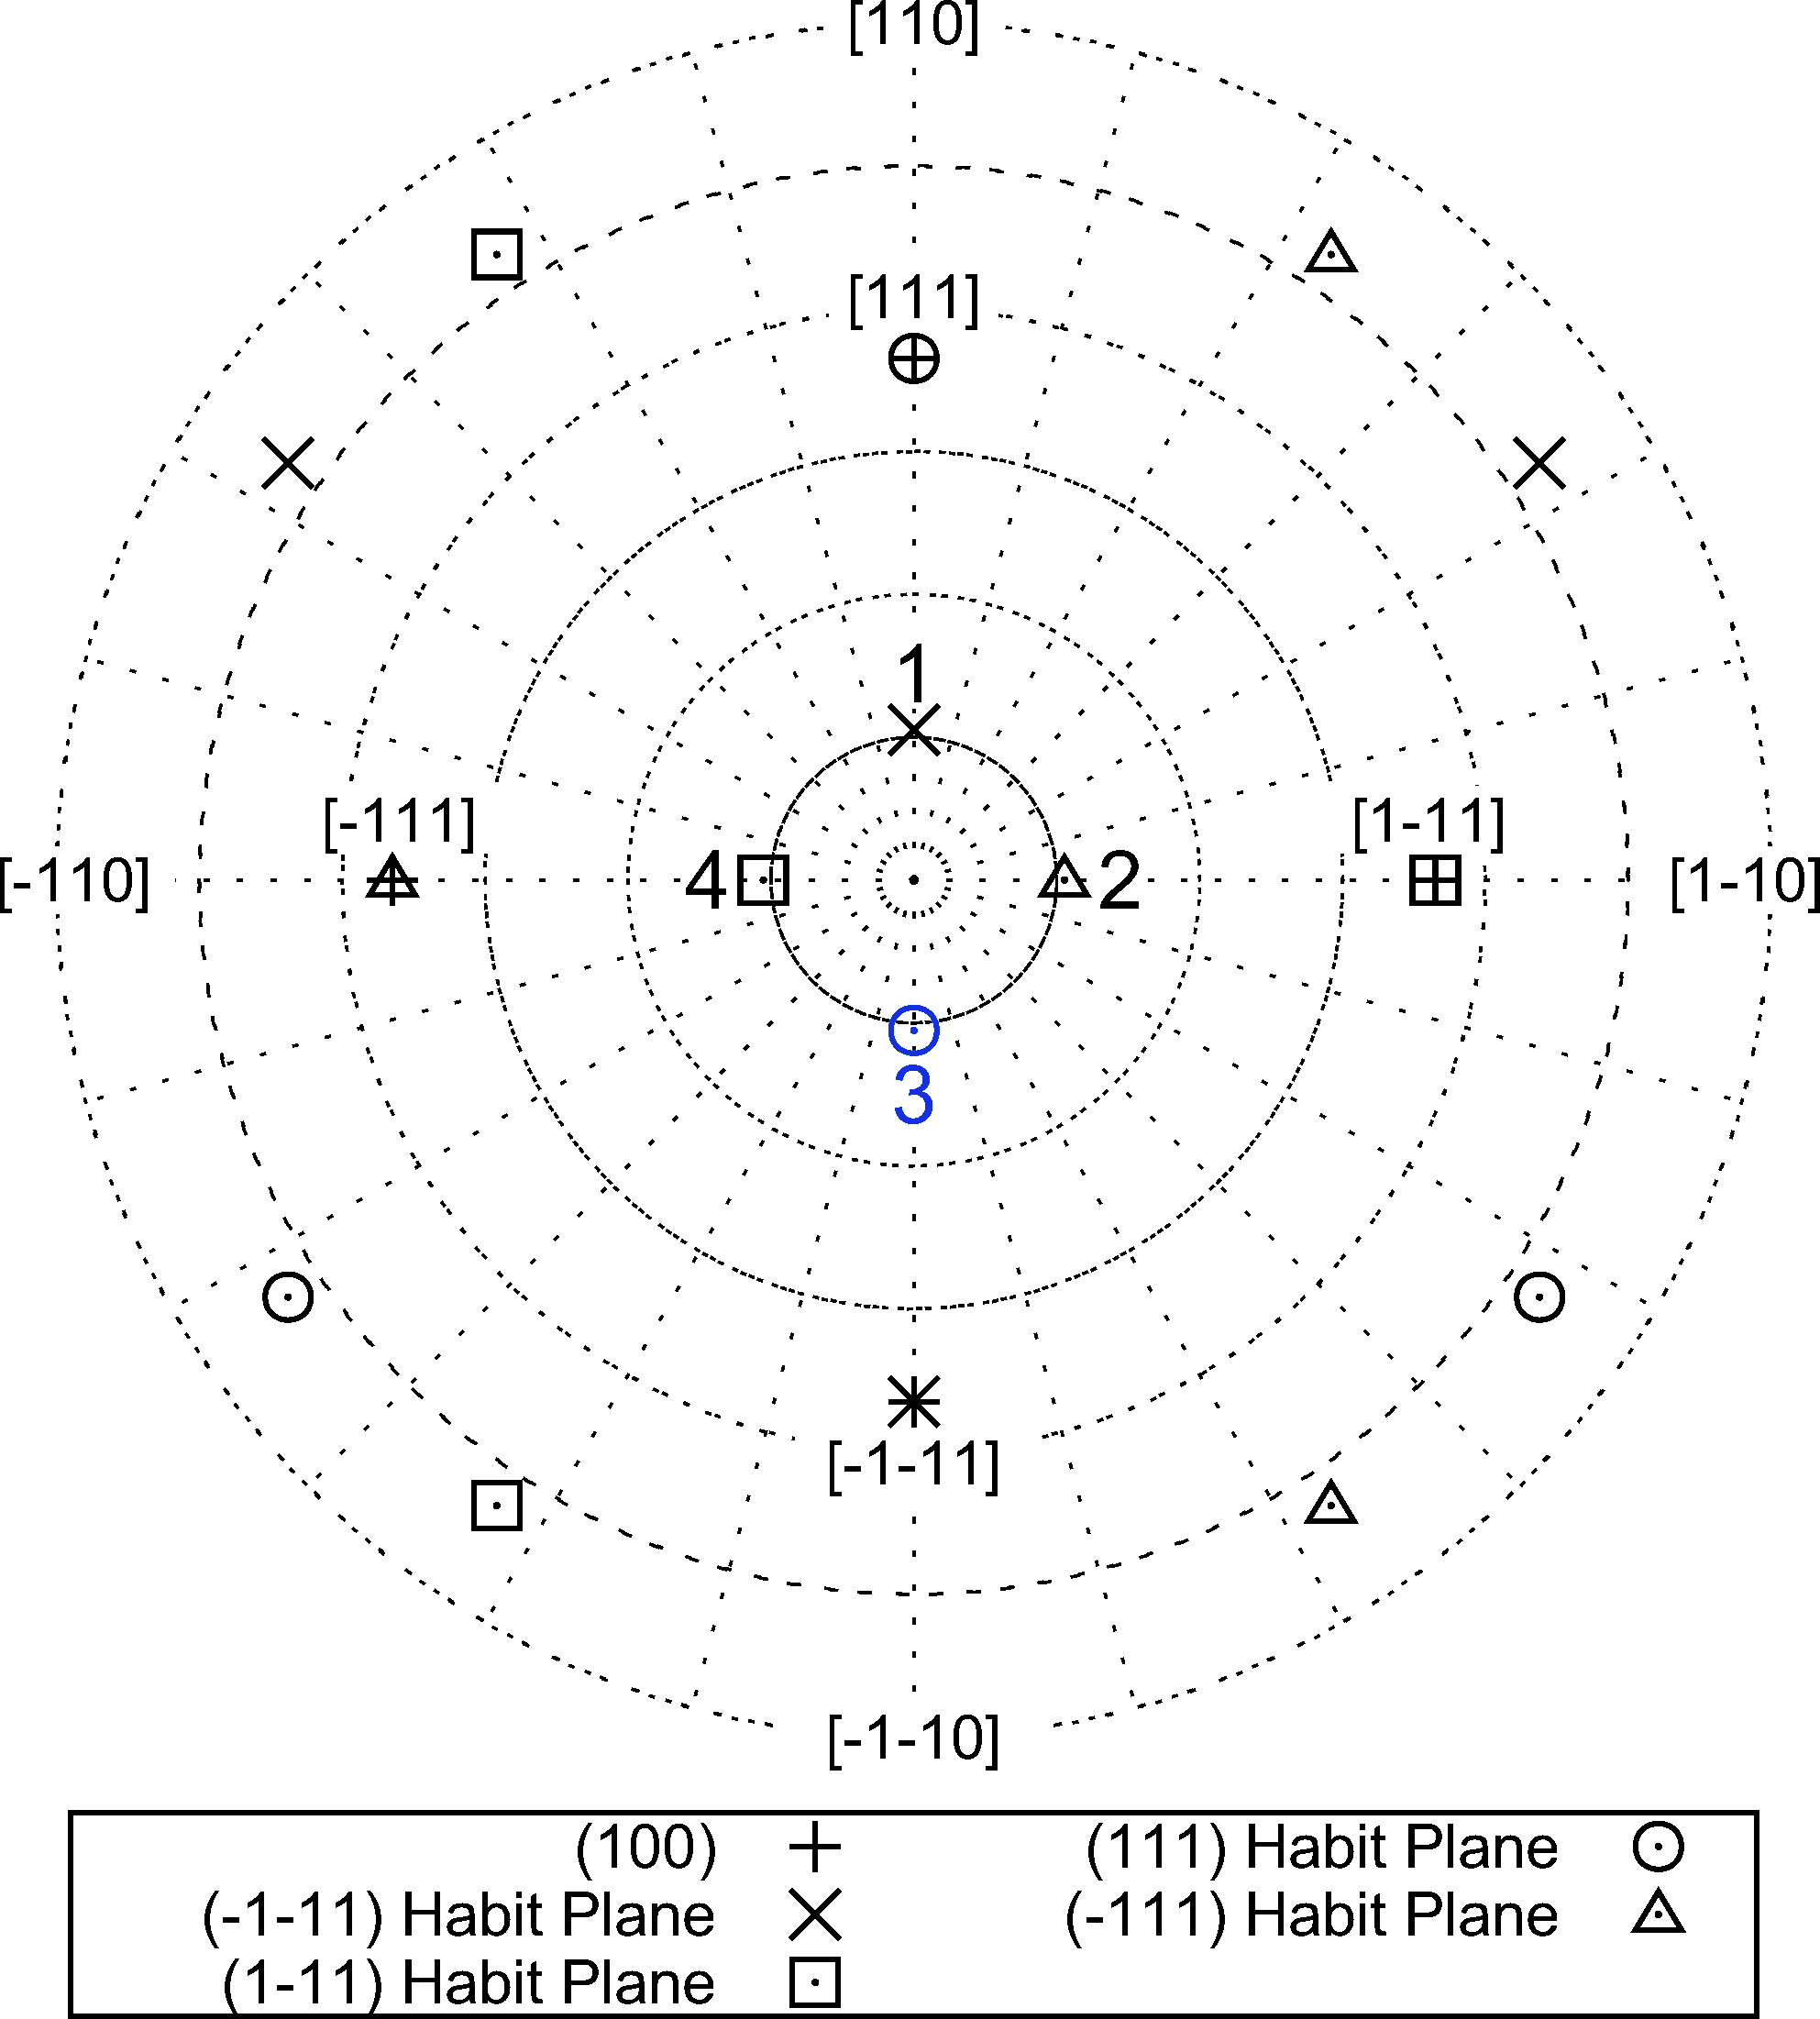
\includegraphics[width=\textwidth]{graphics/twins_simulated_polefigure_highlight}}
            \end{figure}
        \end{column}
        \begin{column}{0.5\textwidth}
            \begin{figure}
                \only<1>{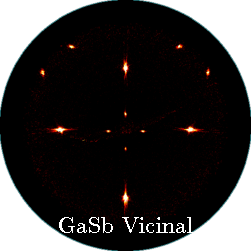
\includegraphics[width=\textwidth]{graphics/gasb_pole}\vspace{0.6cm}}
                \only<2>{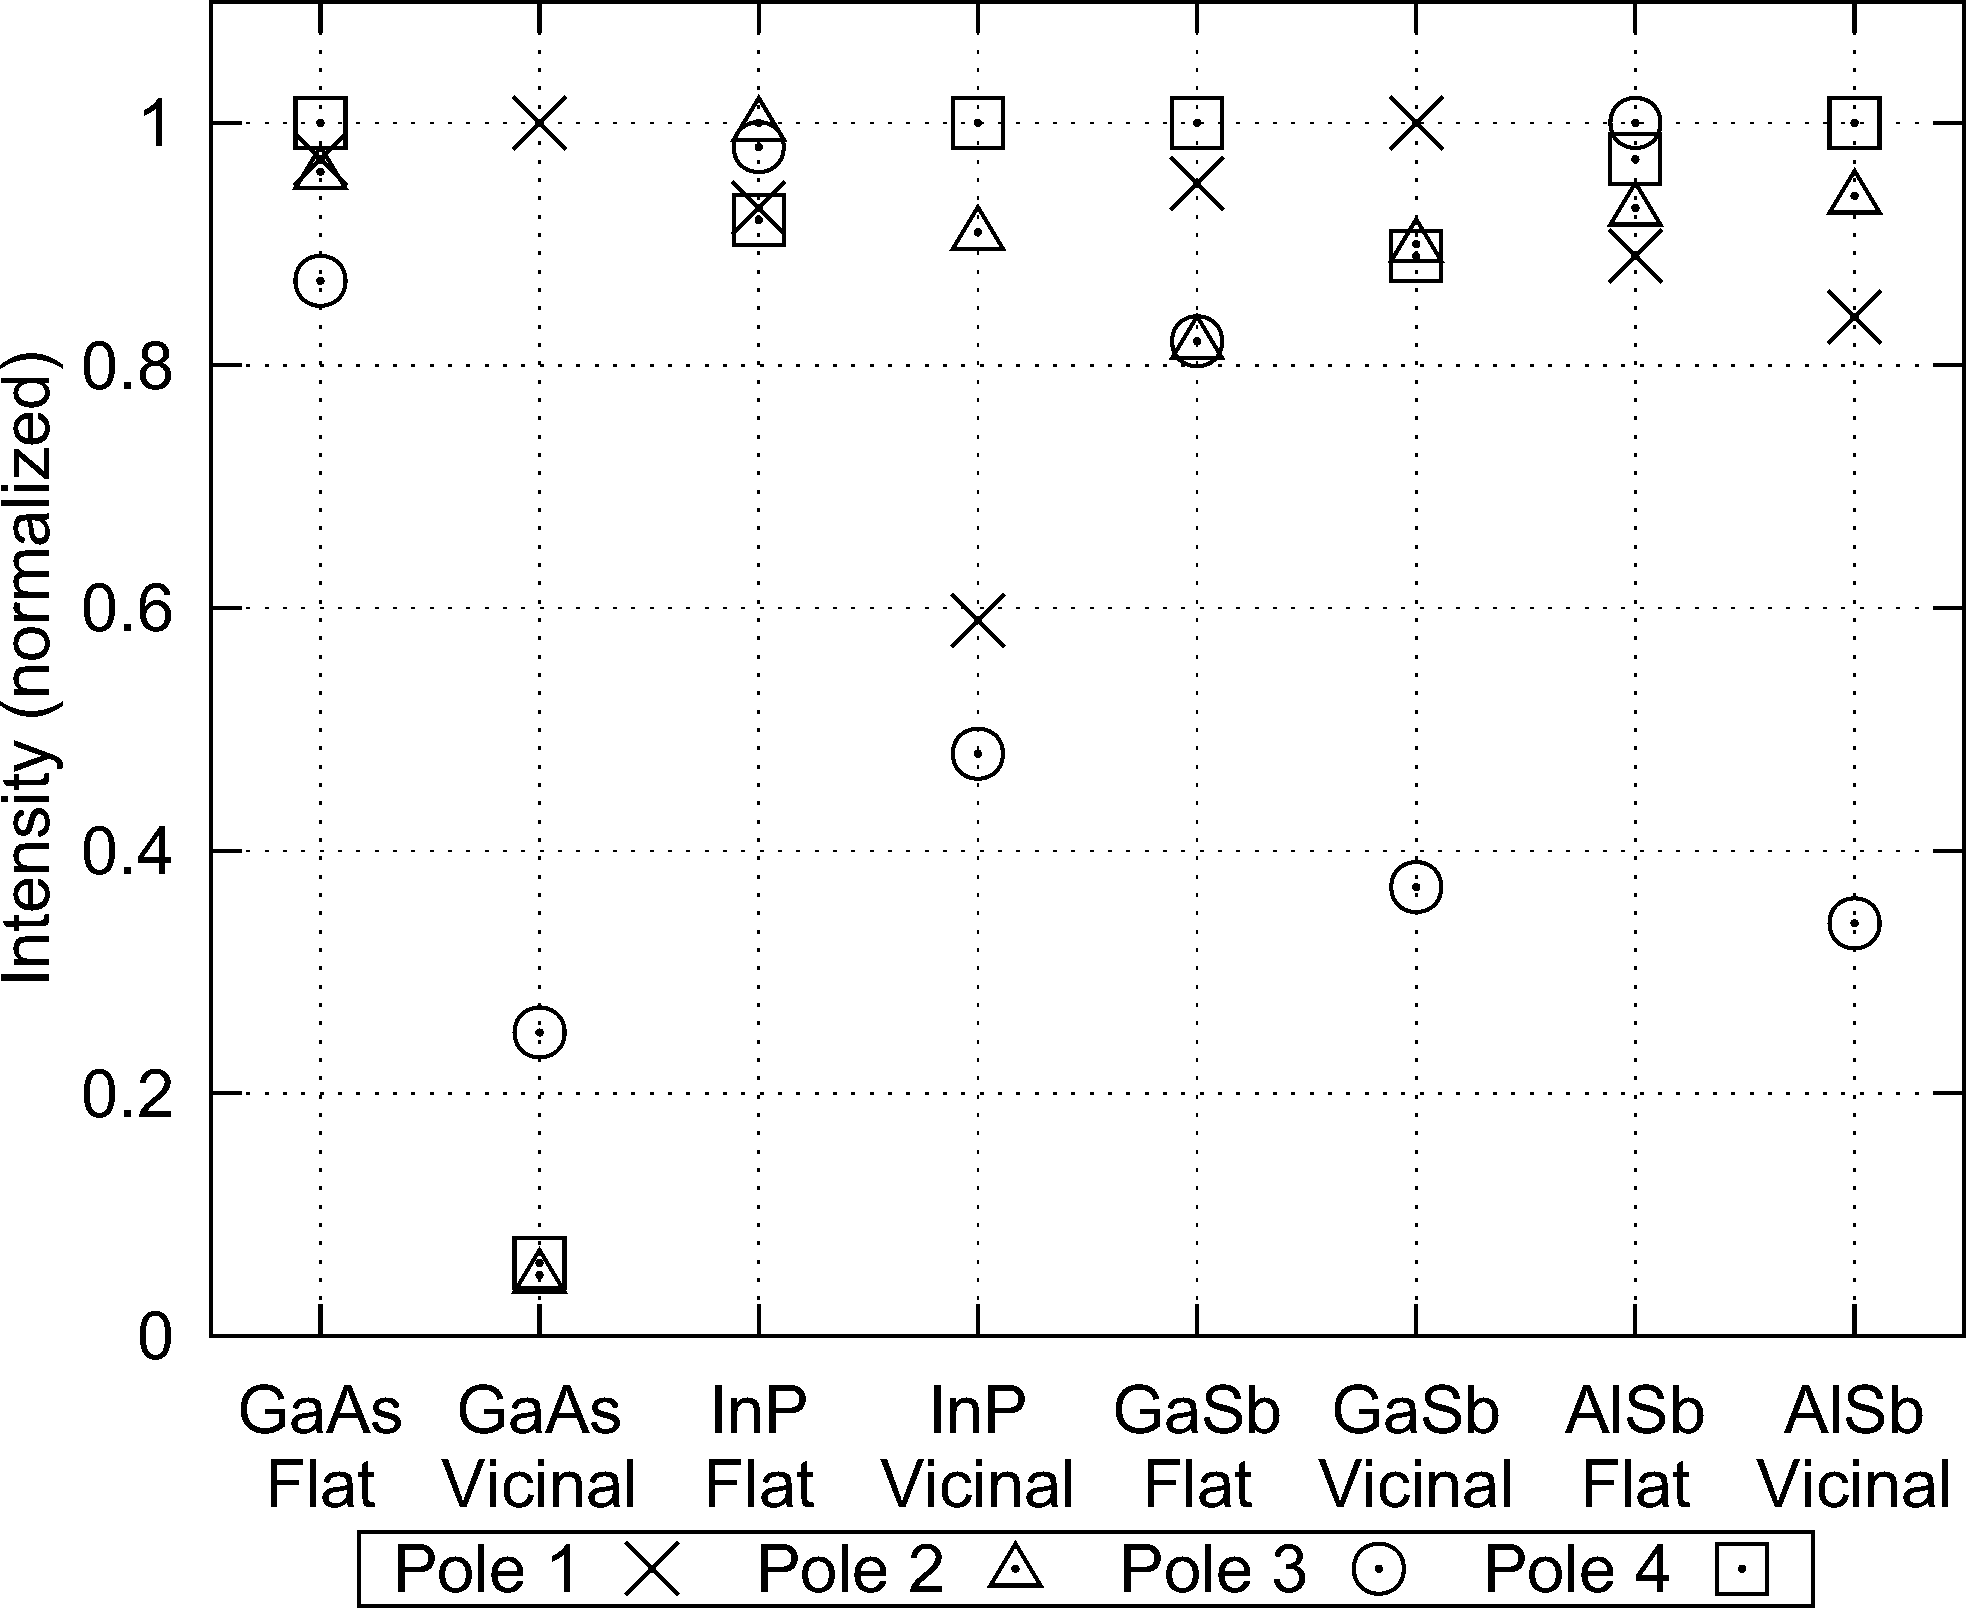
\includegraphics[width=\textwidth]{graphics/twins_intensity}}
                \only<3>{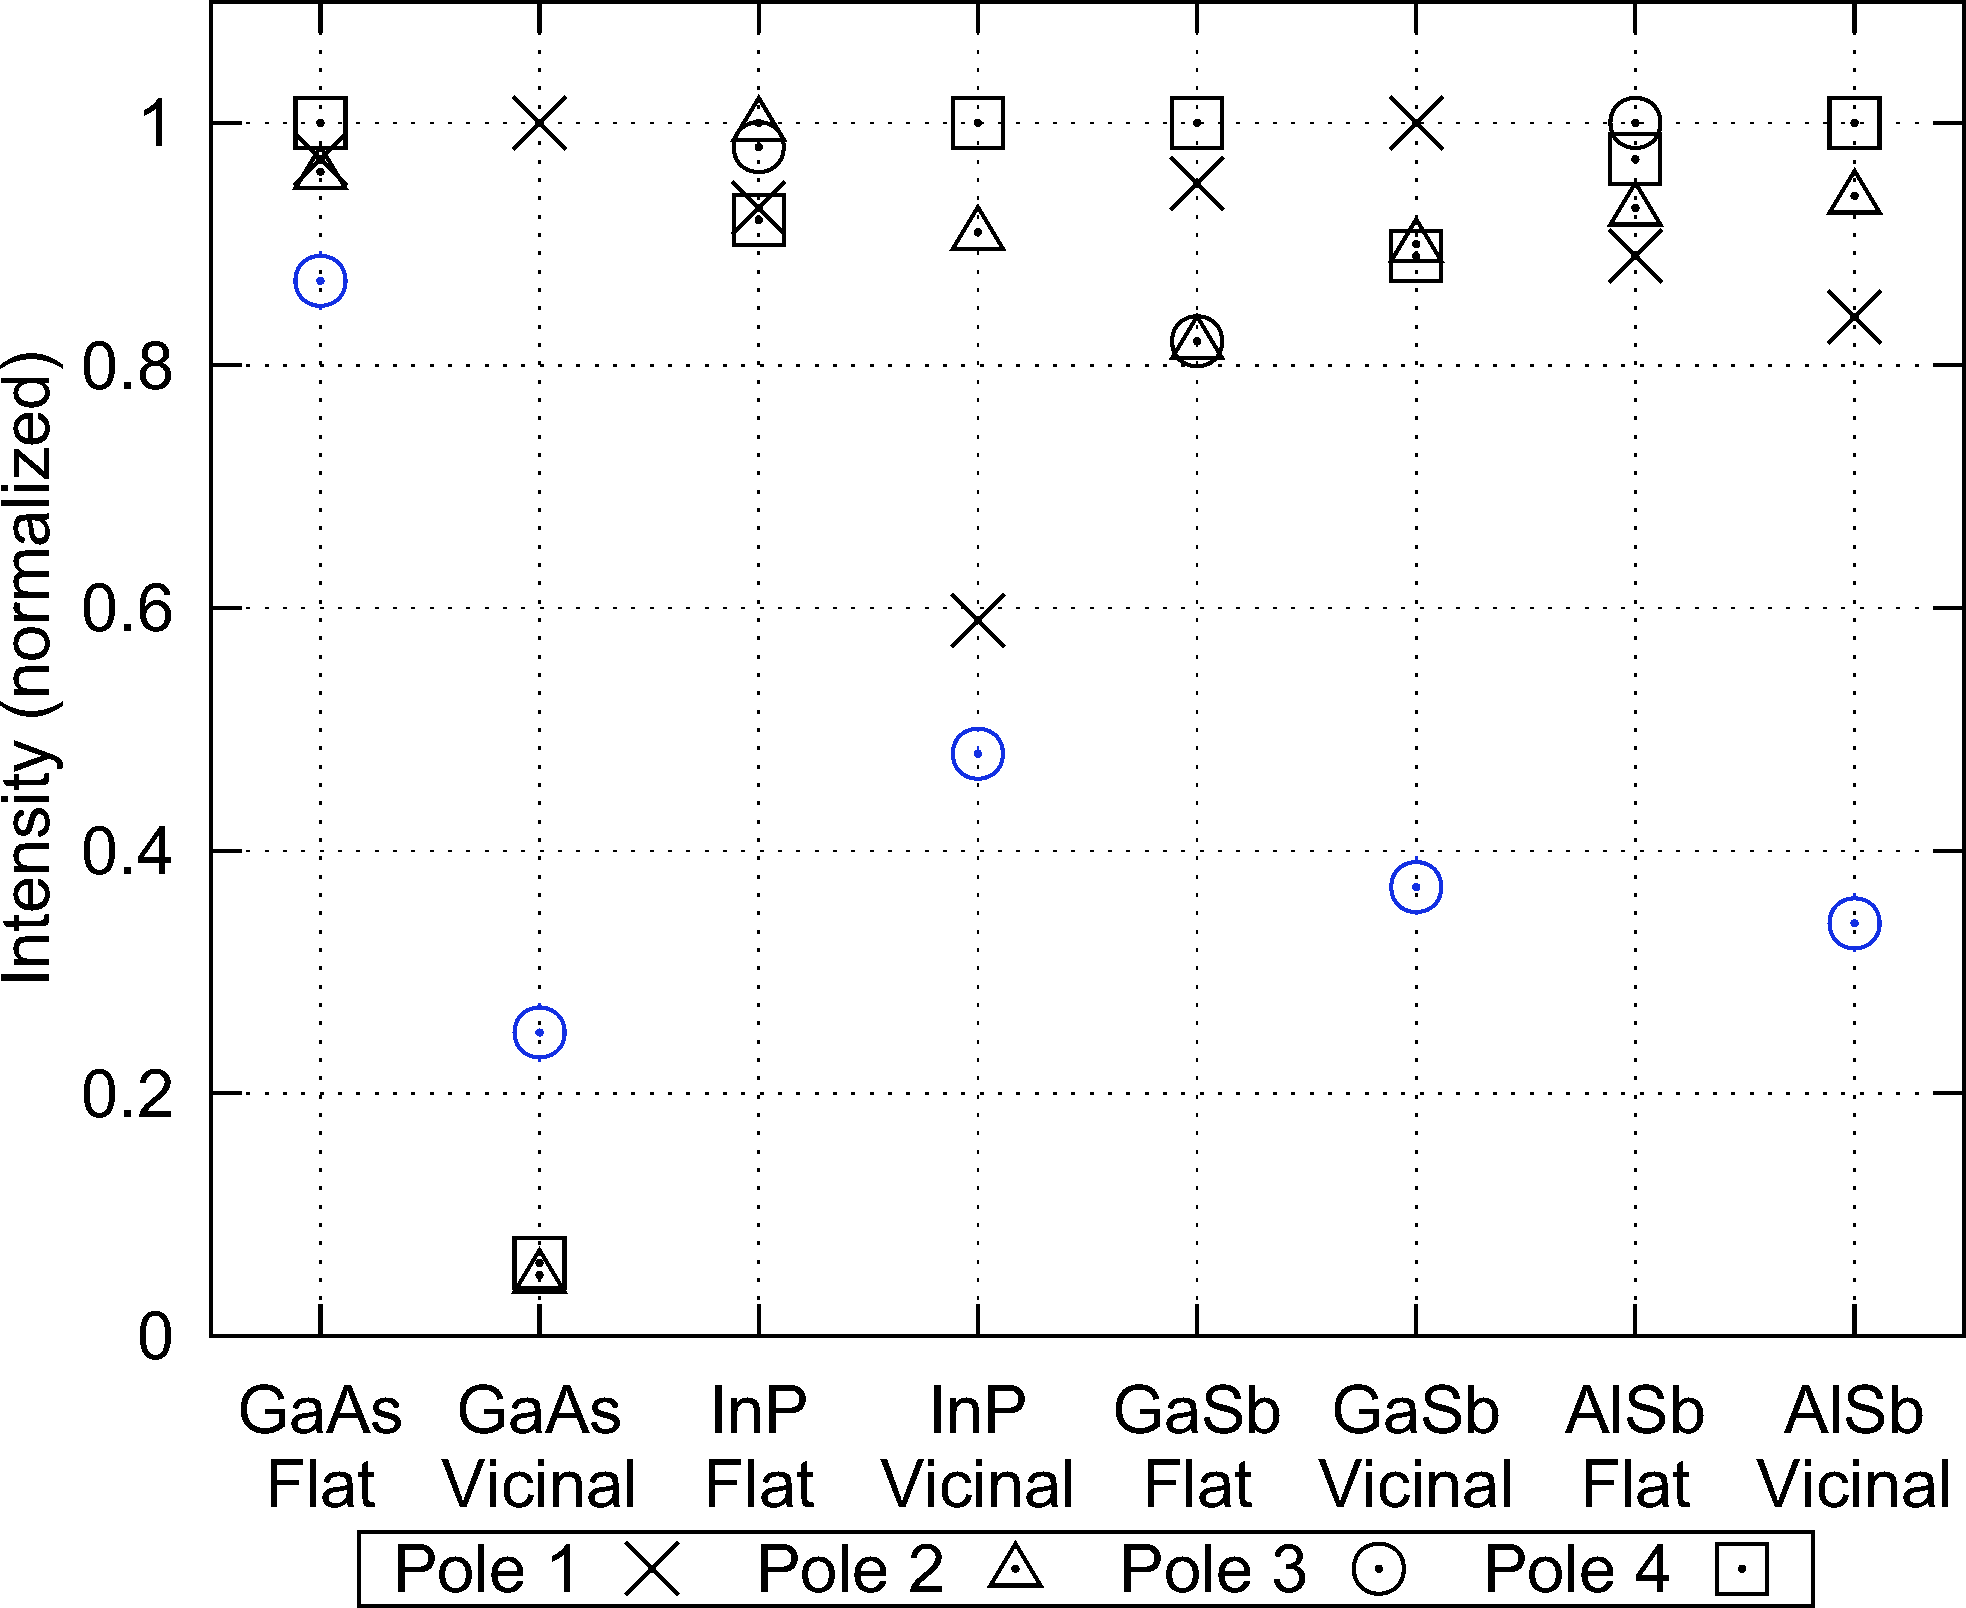
\includegraphics[width=\textwidth]{graphics/twins_intensity_highlight}}
            \end{figure}
        \end{column}
    \end{columns}
\end{frame}

\begin{frame}
    \frametitle{(110) TEM}
    \begin{center}
        \only<1>{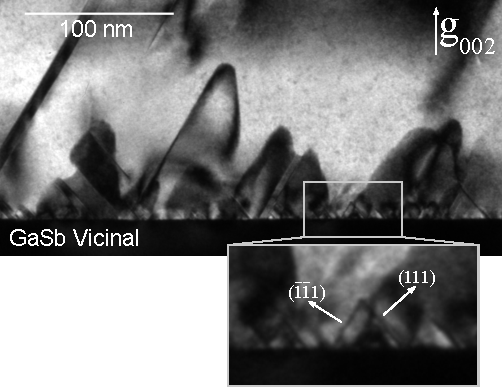
\includegraphics[width=0.85\textwidth]{graphics/twins_TEM}}
        \only<2>{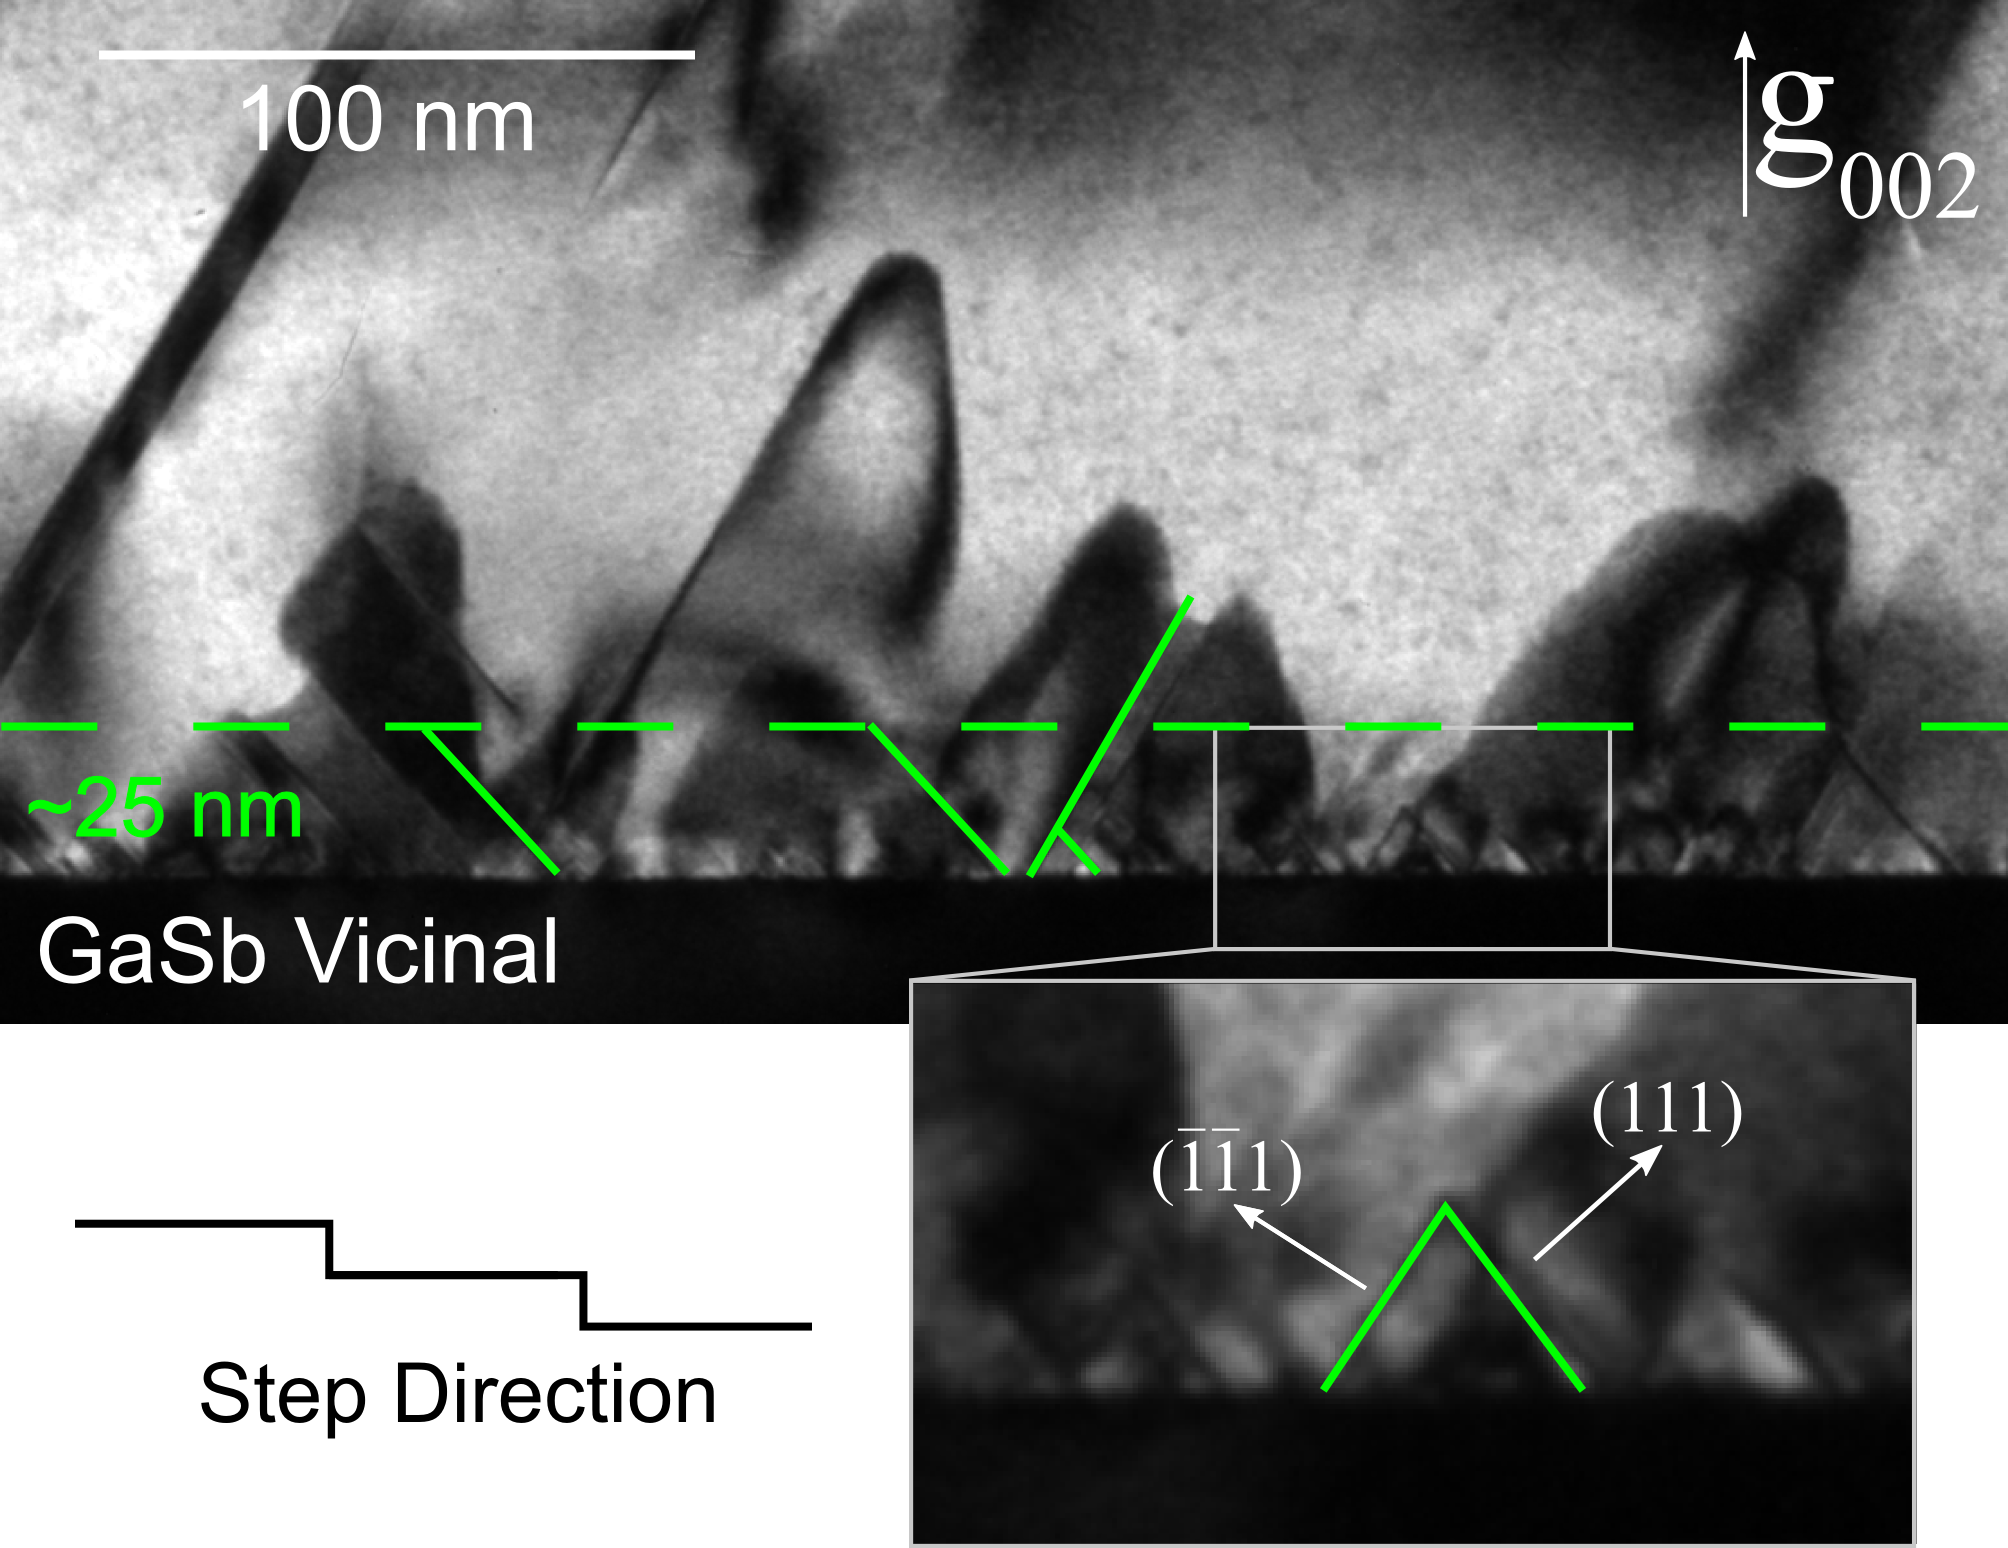
\includegraphics[width=0.85\textwidth]{graphics/twins_TEM_labelled}}
    \end{center}
\end{frame}

\begin{frame}
    \frametitle{Twins Epitaxy on Vicinal (001) Silicon}
    \begin{columns}[C]
        \begin{column}{0.5\textwidth}
    \begin{block}{Conclusions}
        \begin{itemize}[<+-| alert@+>]
            \item Twins form on all <111> surfaces
             \item Vicinal substrates cause asymmetric step formation in (001) silicon substrates
             \item Steps on the surface enhances the growth rate away from step edges
            \item Asymmetric growth rate overgrows twins limiting to a thin layer at the interface
        \end{itemize}
    \end{block}
\end{column}
\begin{column}{0.5\textwidth}
    \centering
    \visible<1->{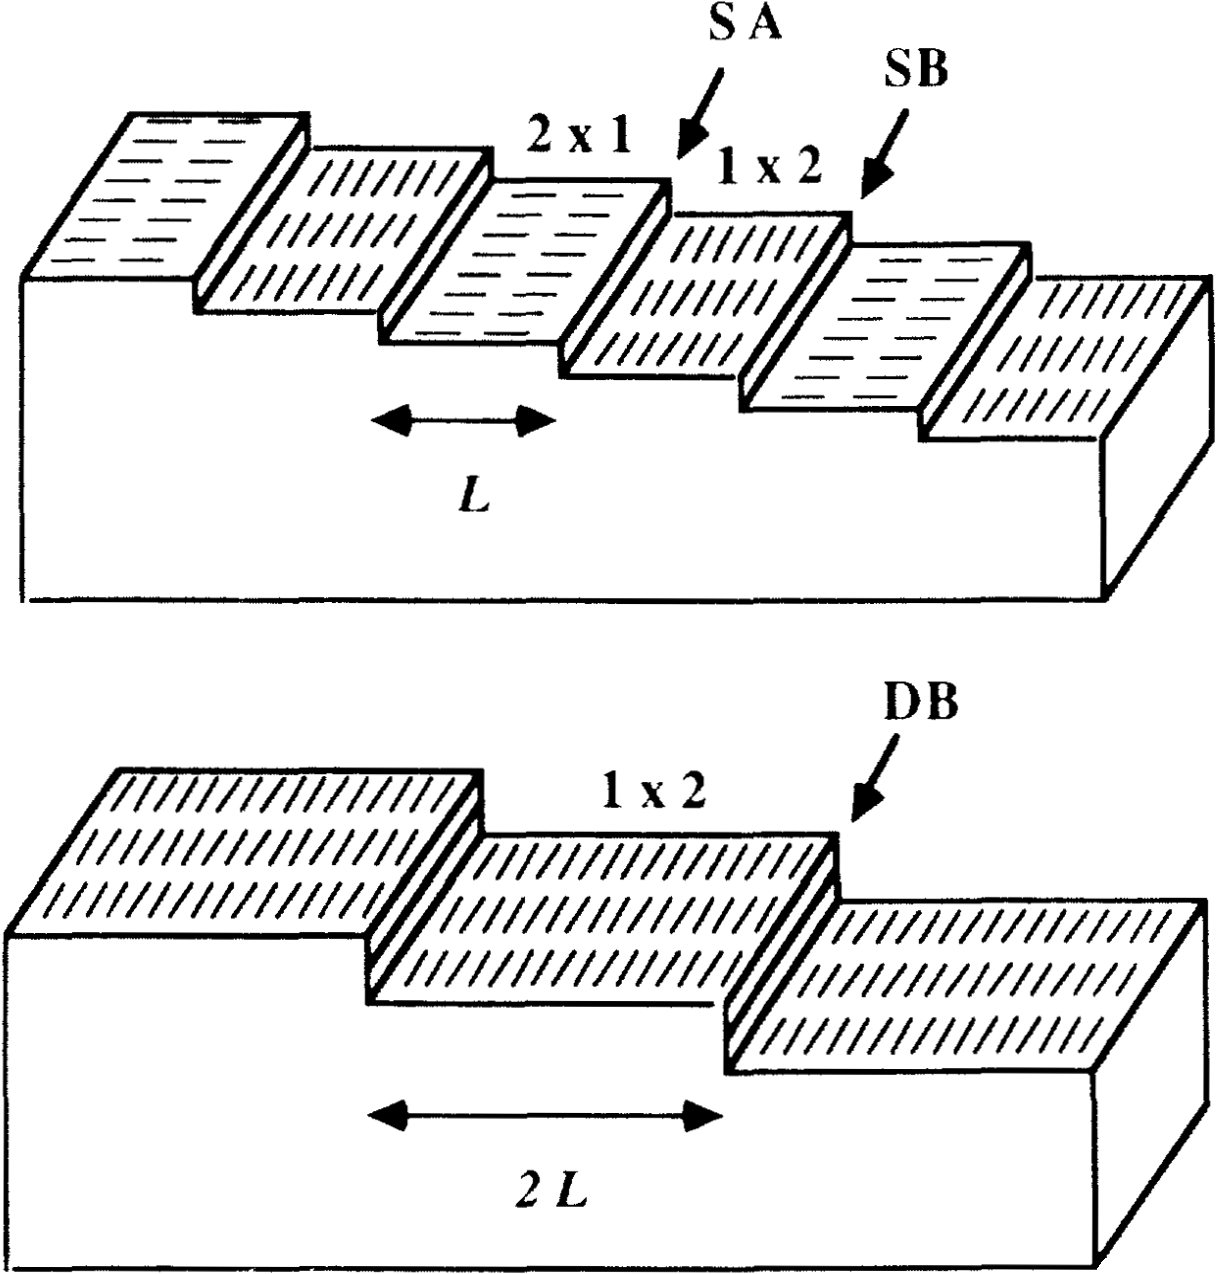
\includegraphics[width=0.7\textwidth]{graphics/back_recon_vicinal}\\ \TINY O. Alerhand, et. al.,  Phys. Rev. Lett., vol. 64, no. 20, pp. 2406–2409, May 1990.}\vspace{0.25cm} \\
    \visible<2->{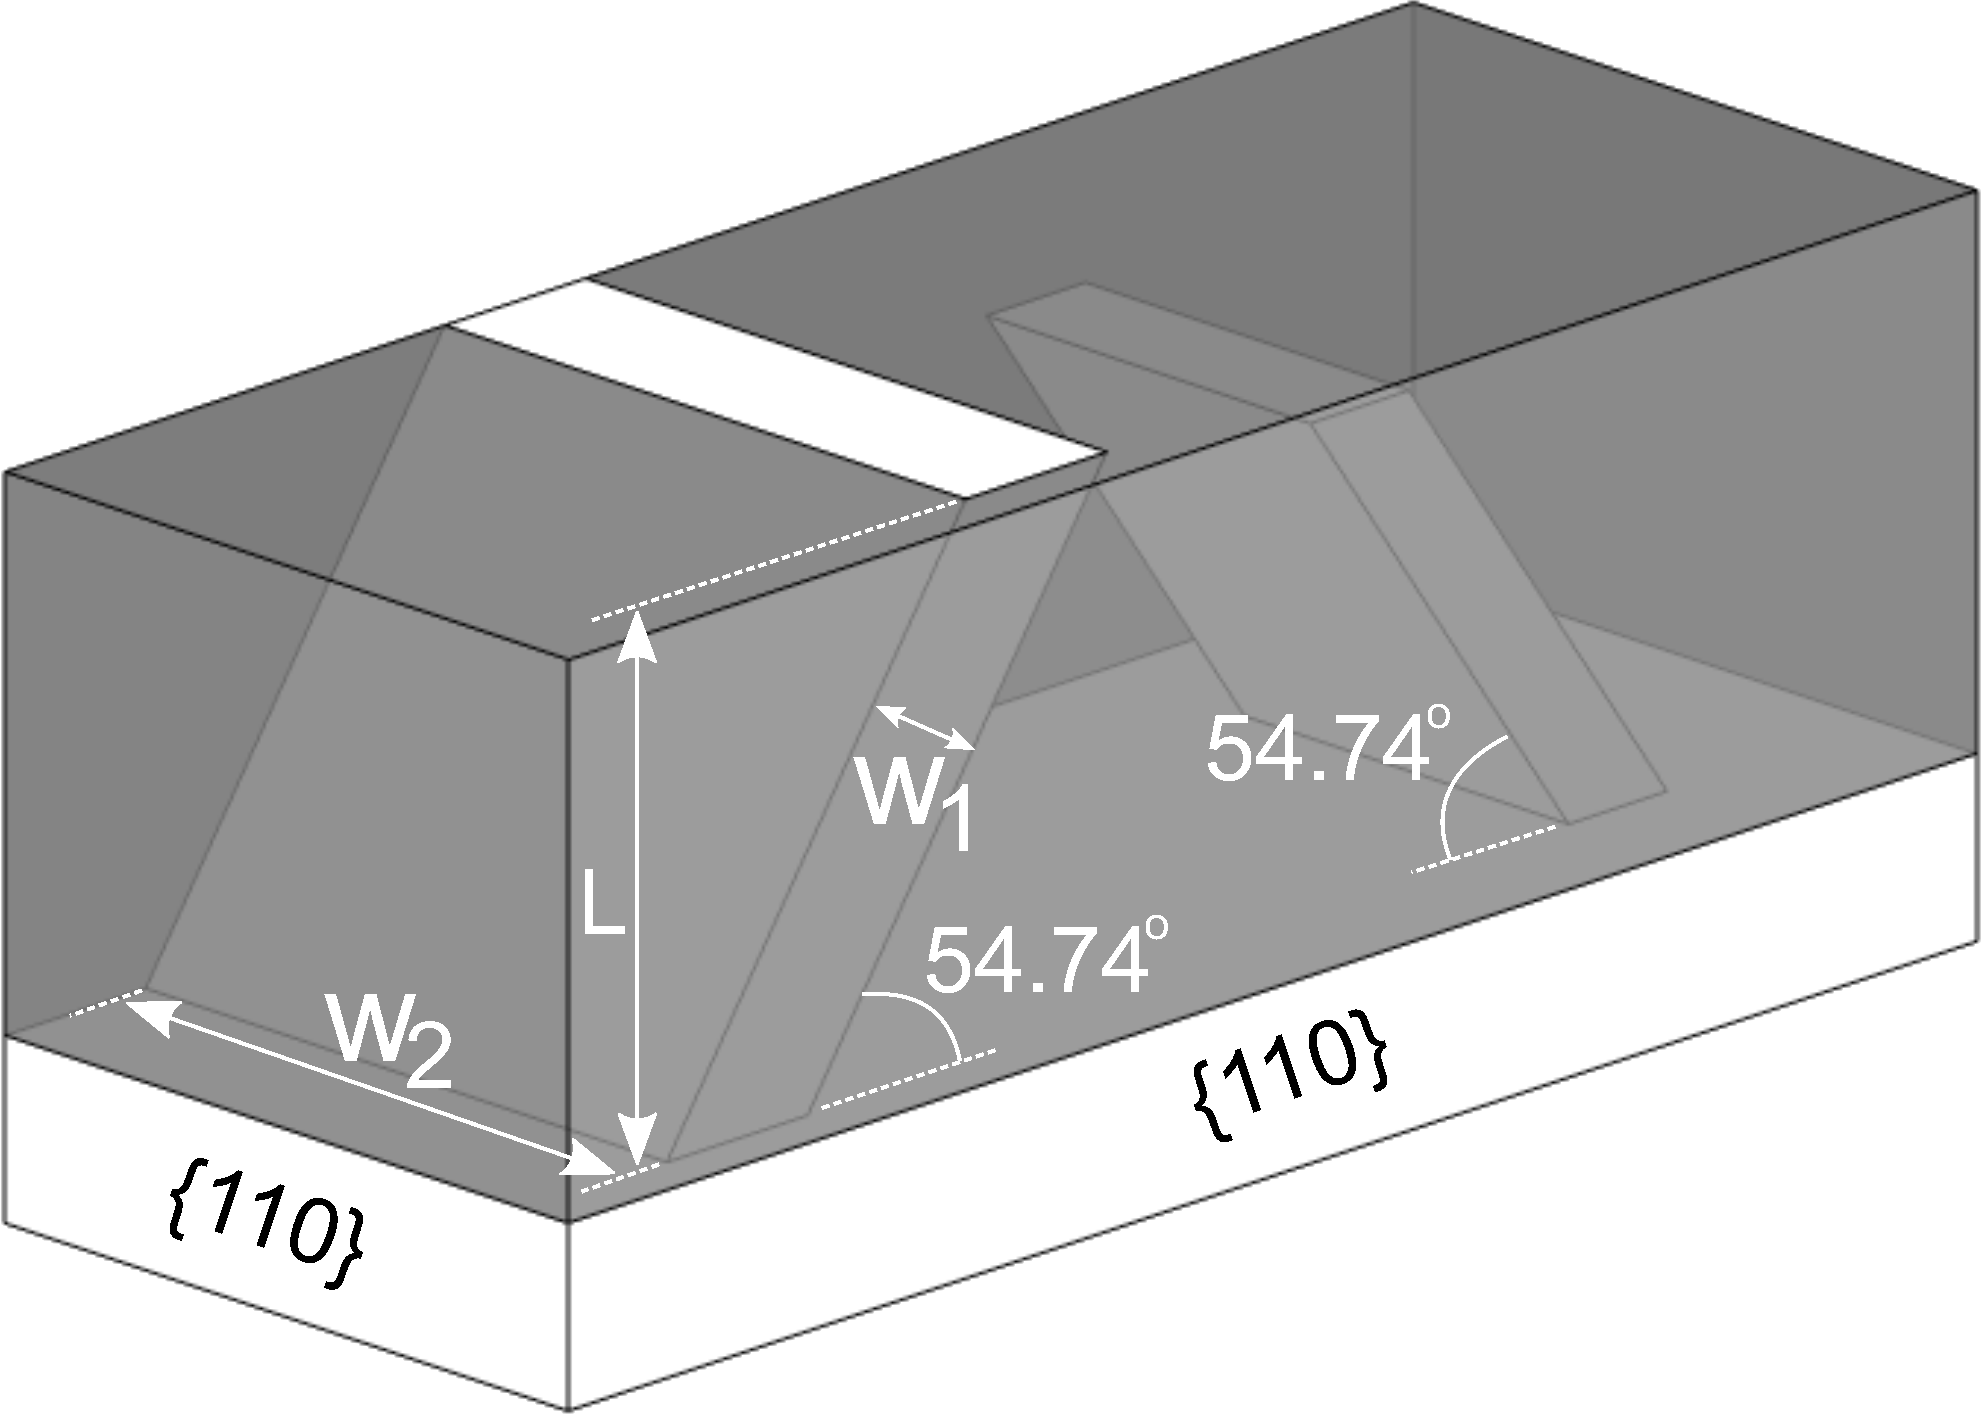
\includegraphics[height=0.35\textheight]{graphics/twins_model}}
    \end{column}
    \end{columns}
\end{frame}

\subsection{Tilted Epitaxy on (211) Silicon}
\begin{frame}
    \frametitle{Outline}
    \tableofcontents[currentsection,currentsubsection]
\end{frame}
\begin{frame}
    \frametitle{Tilted Epitaxy on (211) Silicon}
    \begin{columns}
        \begin{column}{0.5\textwidth}
            \begin{block}{Introduction}
                \begin{itemize}[<+-| alert@+>]
                    \item The (211) surface of cubic diamond crystals are asymmetric, exhibiting atomic stepping
                    \item (211) surfaces also have two non-equivalent lattice sites for zincblende semiconductor nucleation
                    \item (211) substrates were initially investigated to solve the polar on non-polar problem of binary growth on silicon
                \end{itemize}
            \end{block}
        \end{column}
        \begin{column}{0.5\textwidth}
            \centering
            \visible<1->{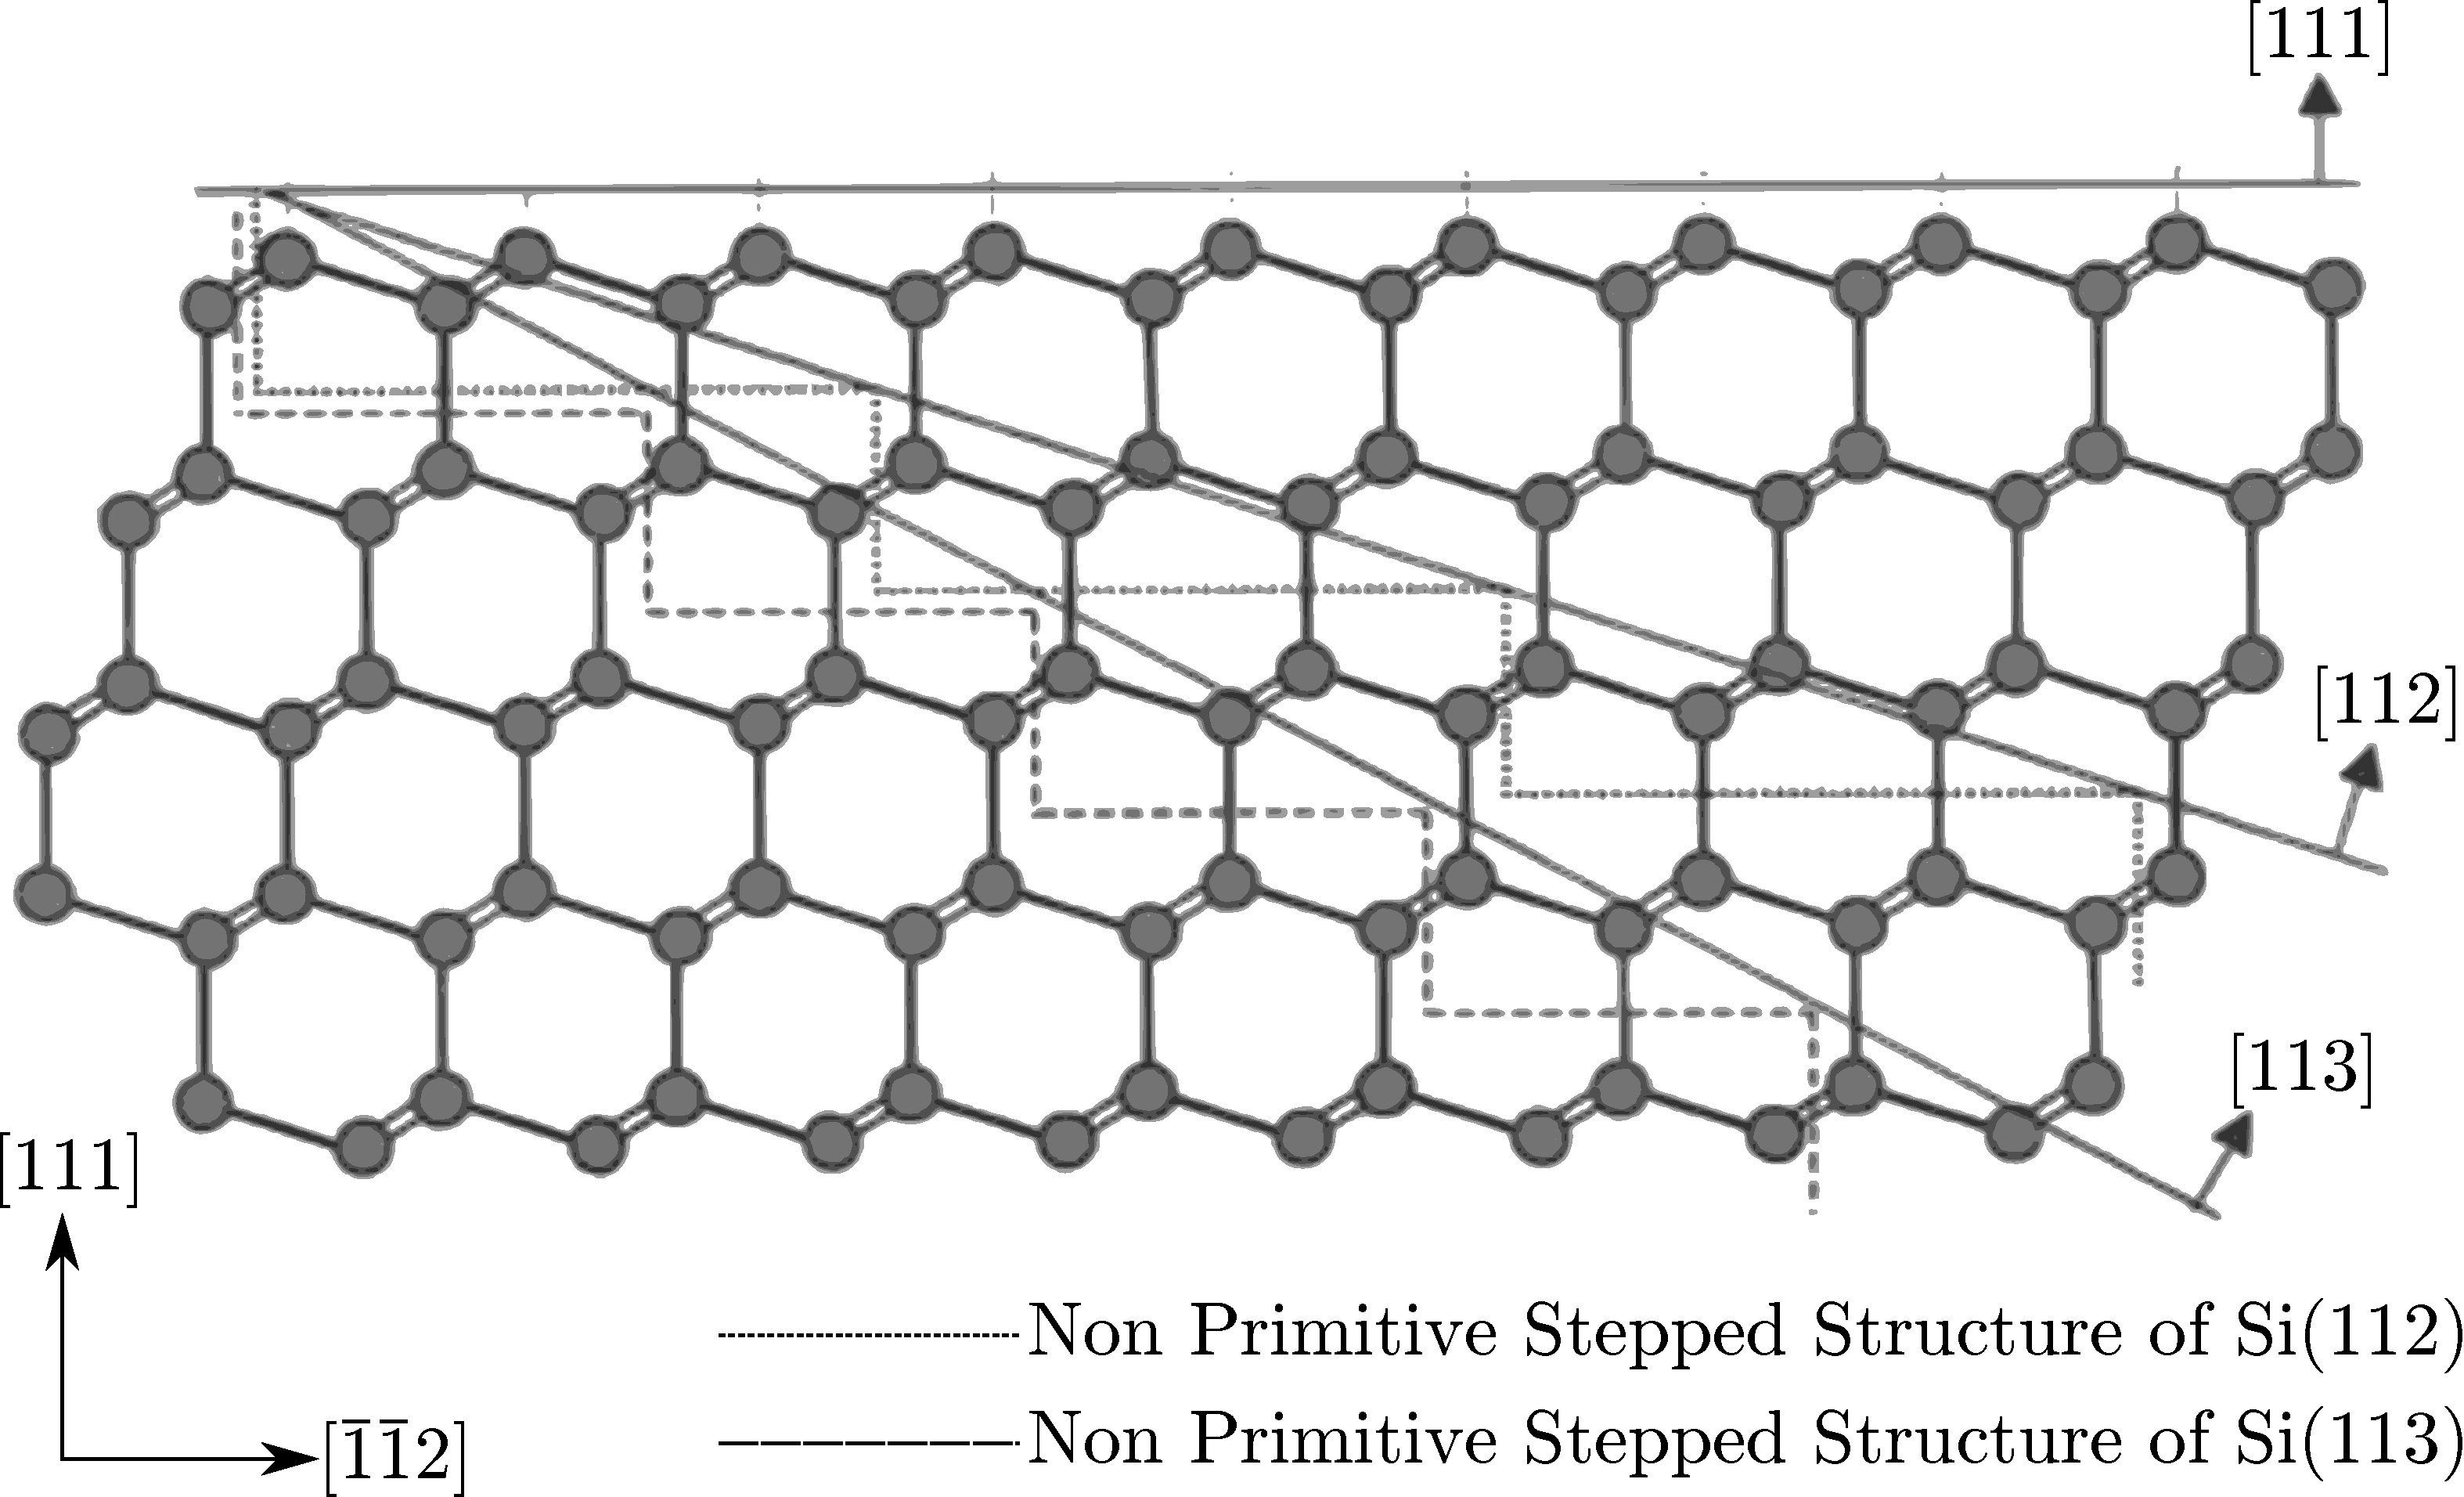
\includegraphics[width=\textwidth]{graphics/211_steps}\\ \TINY G. Brill, et. al., J. Electron. Mater. 32, 717–722 (2003).} \\ \vspace{1cm}
            \visible<2->{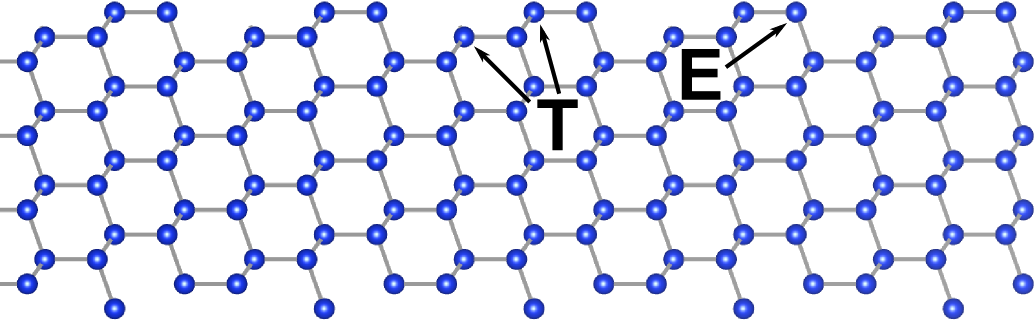
\includegraphics[width=\textwidth]{graphics/211_surface}}
        \end{column}
    \end{columns}
\end{frame}

\begin{frame}
    \frametitle{Tilted Epitaxy on (211) Silicon}
    \begin{columns}
        \begin{column}{0.5\textwidth}
            \begin{block}{Experimental}
                \begin{itemize}[<+-| alert@+>]
                    \item (211) silicon substrates
                    \item 500~nm films of GaSb were deposited in MBE
                    \item GaSb and silicon have an intrinsic lattice mismatch of 13\%
                \end{itemize}
            \end{block}
        \end{column}
        \begin{column}{0.5\textwidth}
            \centering
            \only<1>{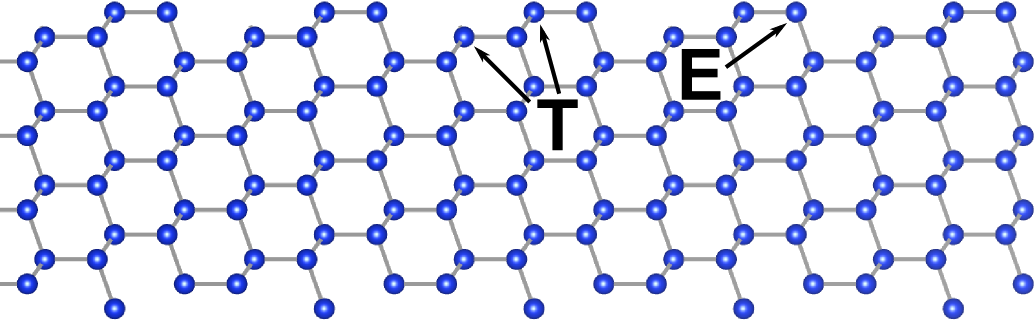
\includegraphics[width=\textwidth]{graphics/211_surface}}
            \only<2->{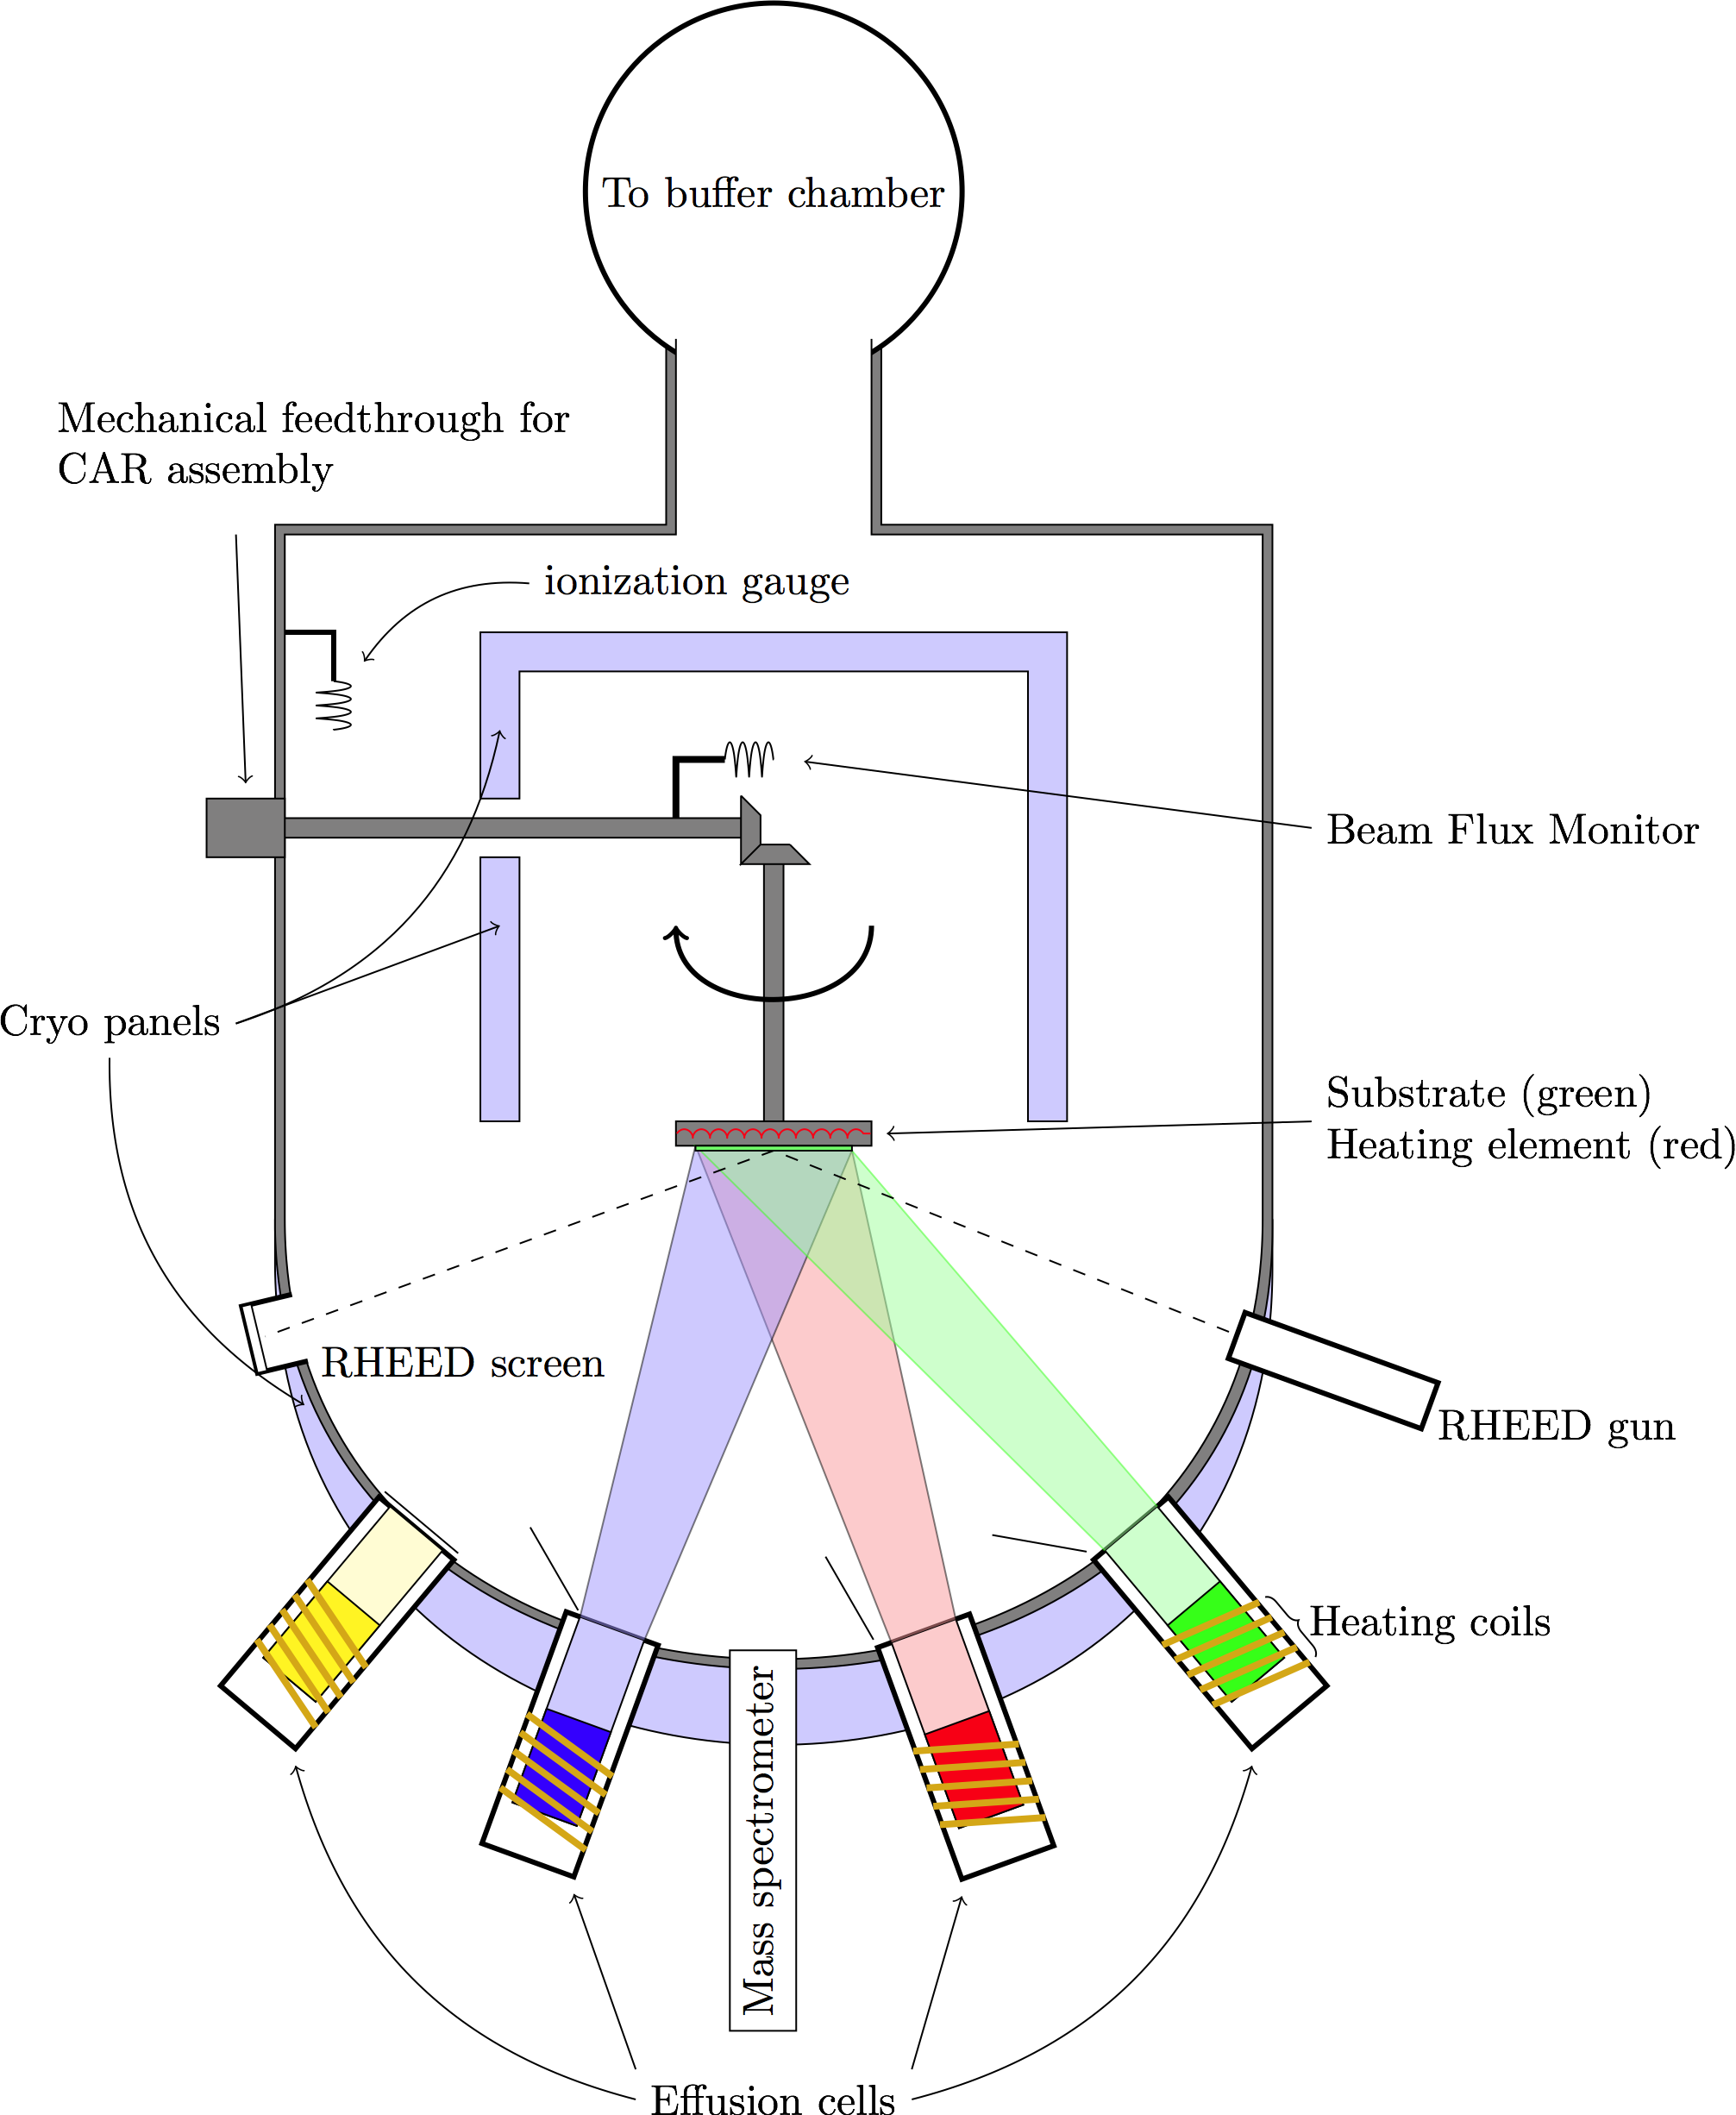
\includegraphics[width=\textwidth]{graphics/MBE}}
        \end{column}
    \end{columns}
\end{frame}

\begin{frame}
    \frametitle{2DXRD Results}
    \begin{center}
    \only<1>{
    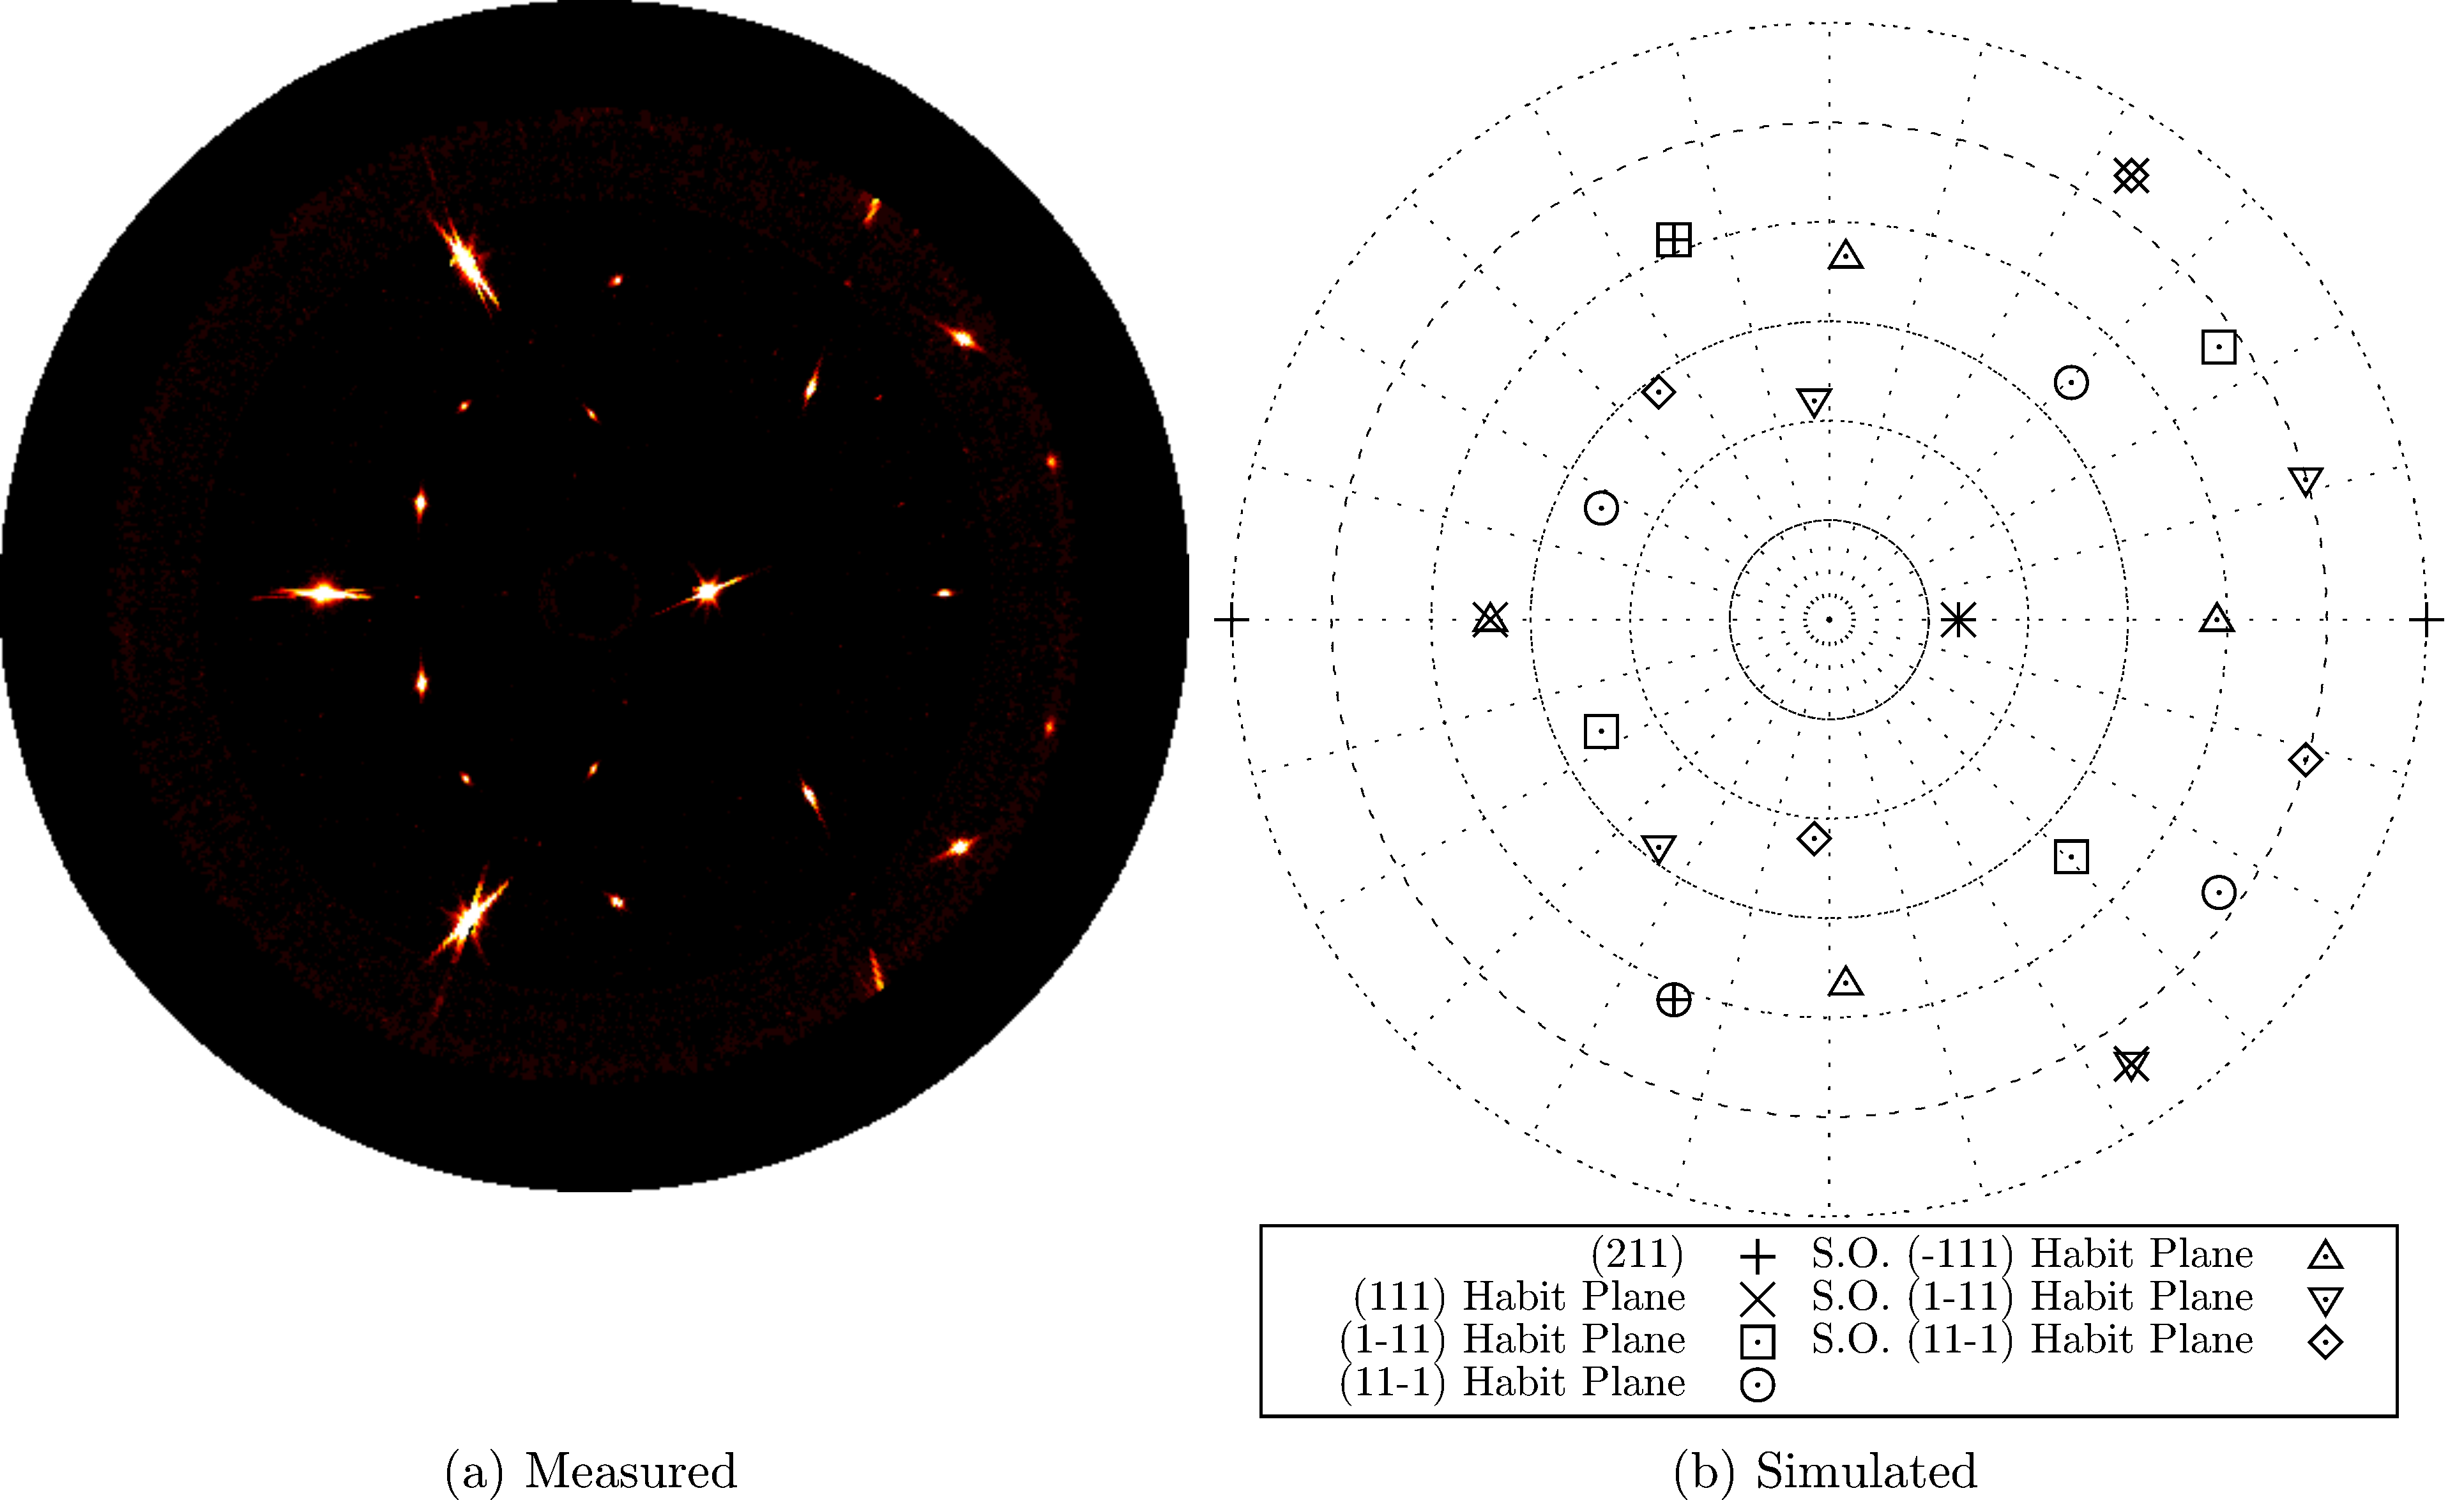
\includegraphics[width=\textwidth]{graphics/211_polefigure}}
    \only<2>{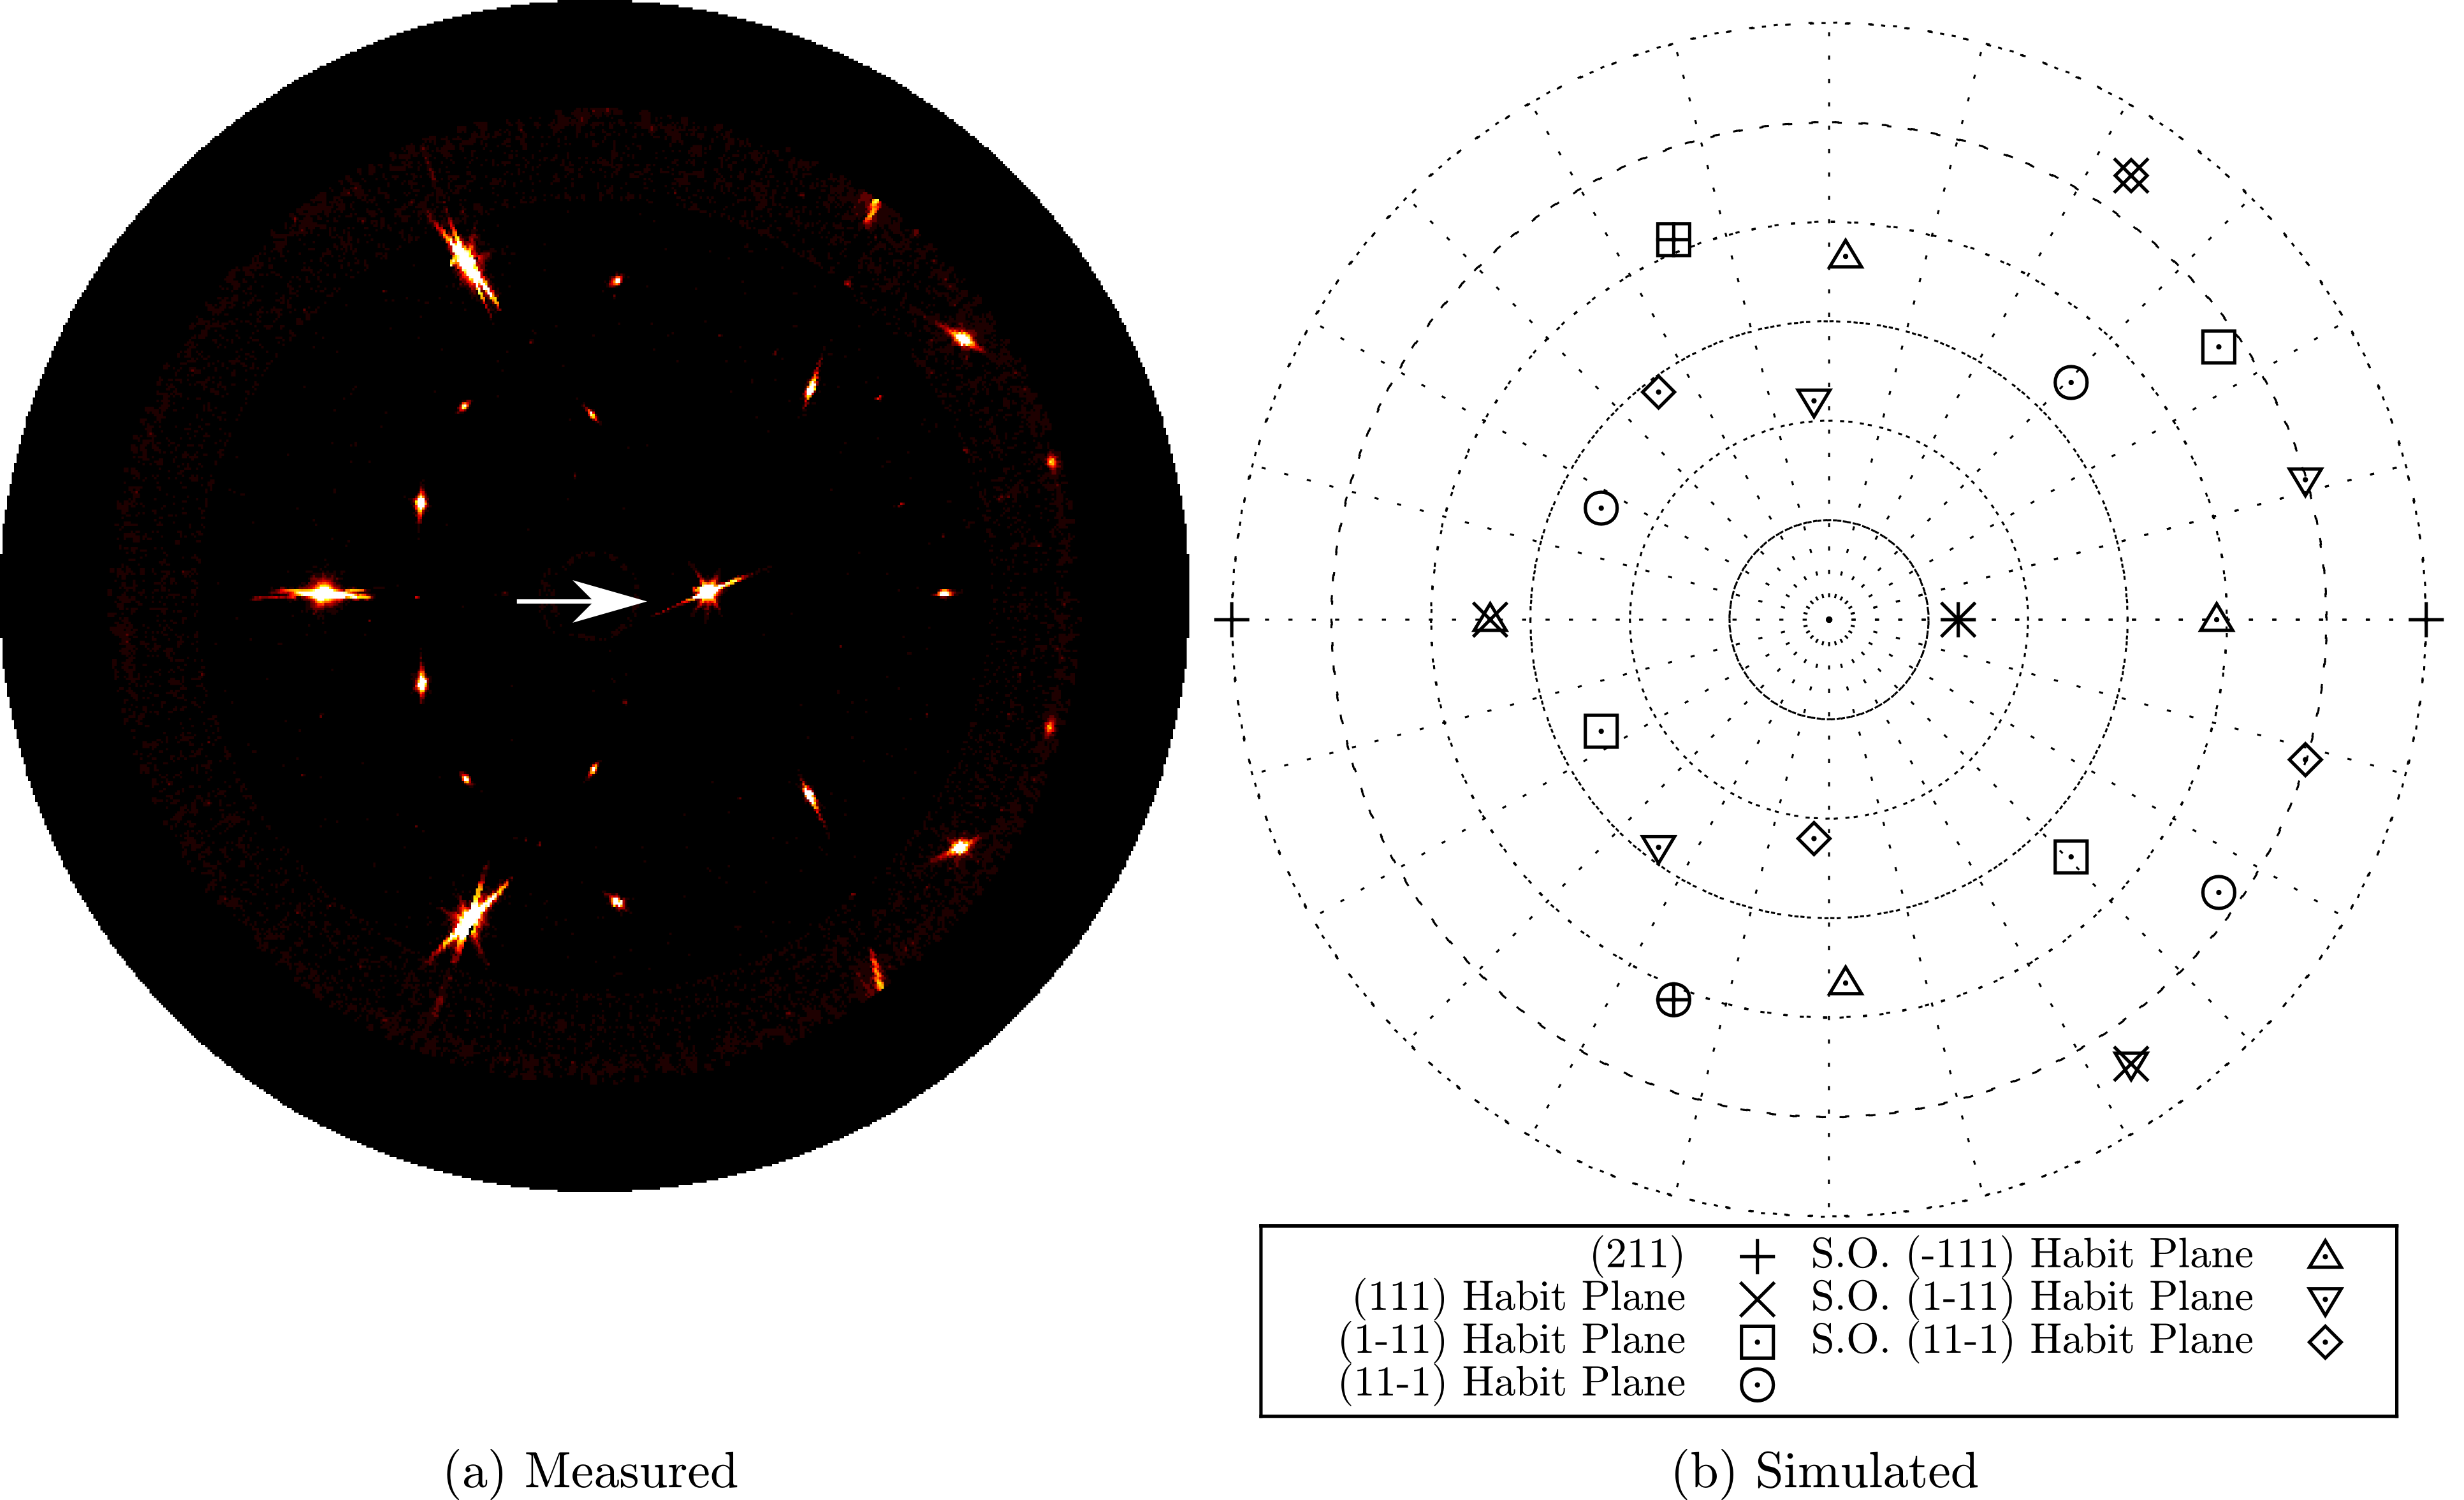
\includegraphics[width=\textwidth]{graphics/211_polefigure_2}}
\end{center}
\end{frame}

\begin{frame}
    \frametitle{A Toy Model}
        \only<1>{\begin{figure}
                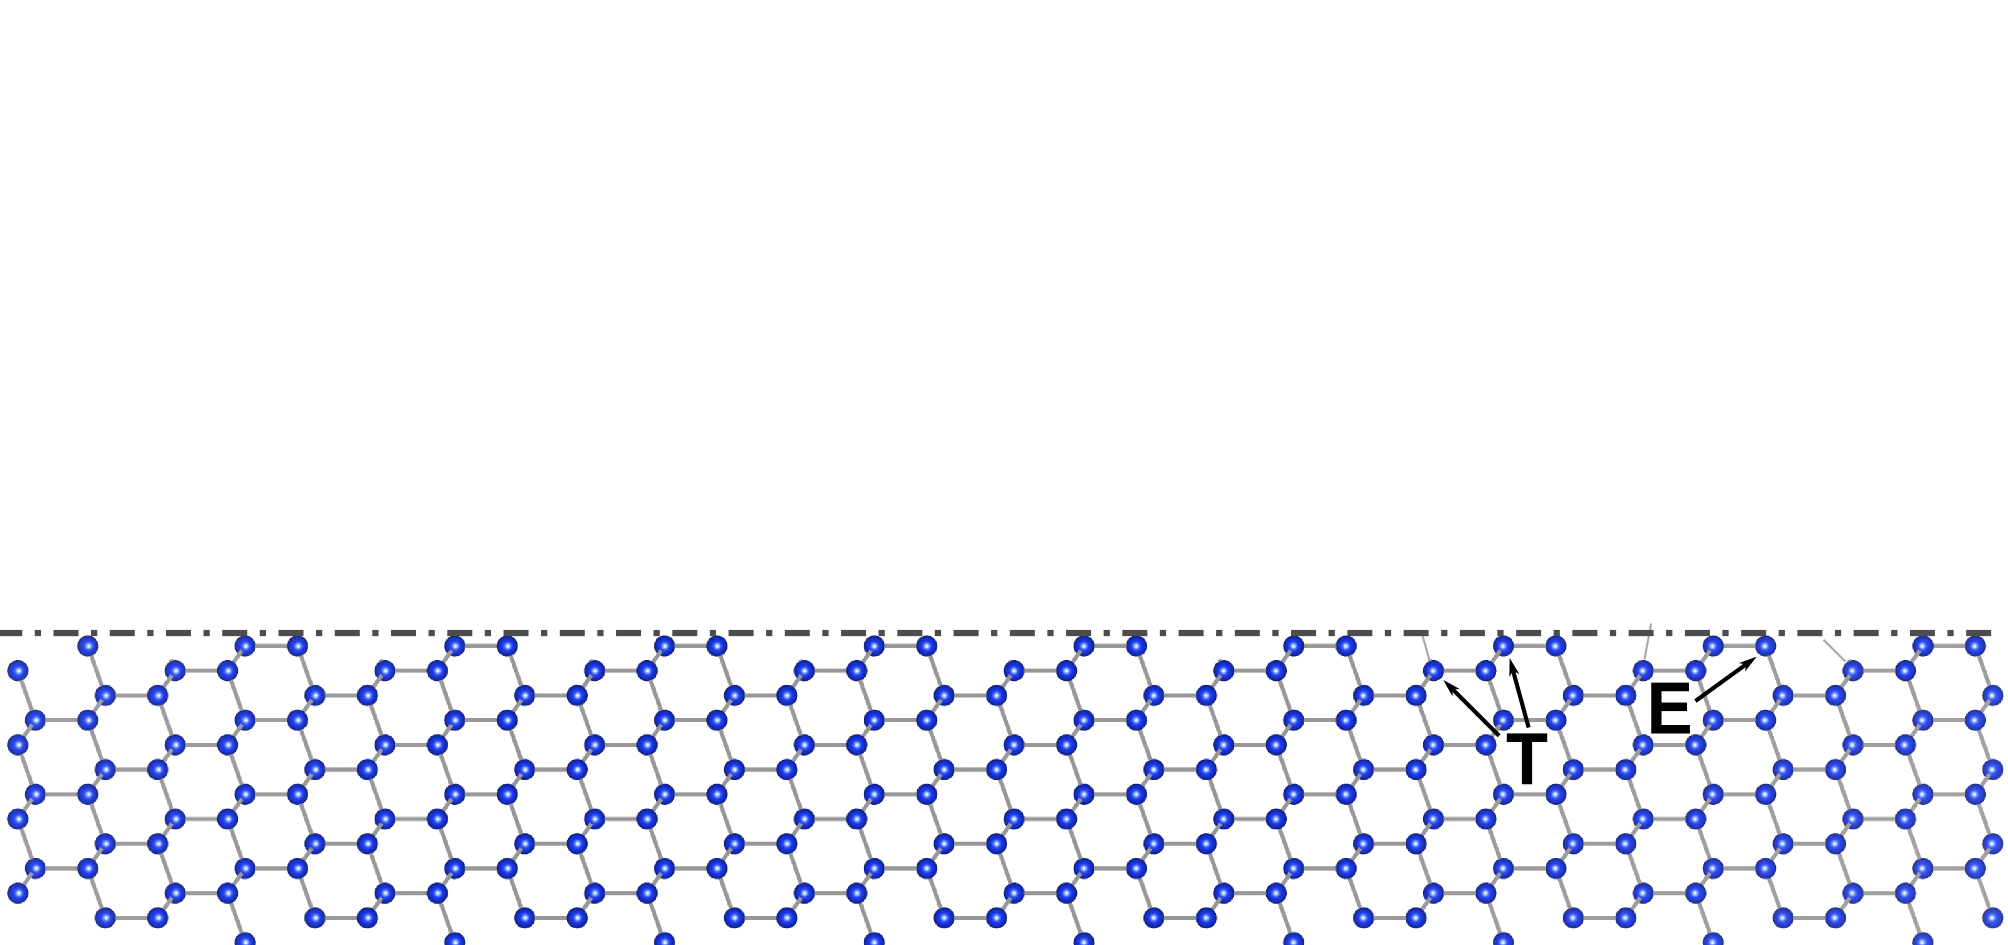
\includegraphics[width=\textwidth]{graphics/211_blank}
            \end{figure}}
        \only<2>{\begin{figure}
            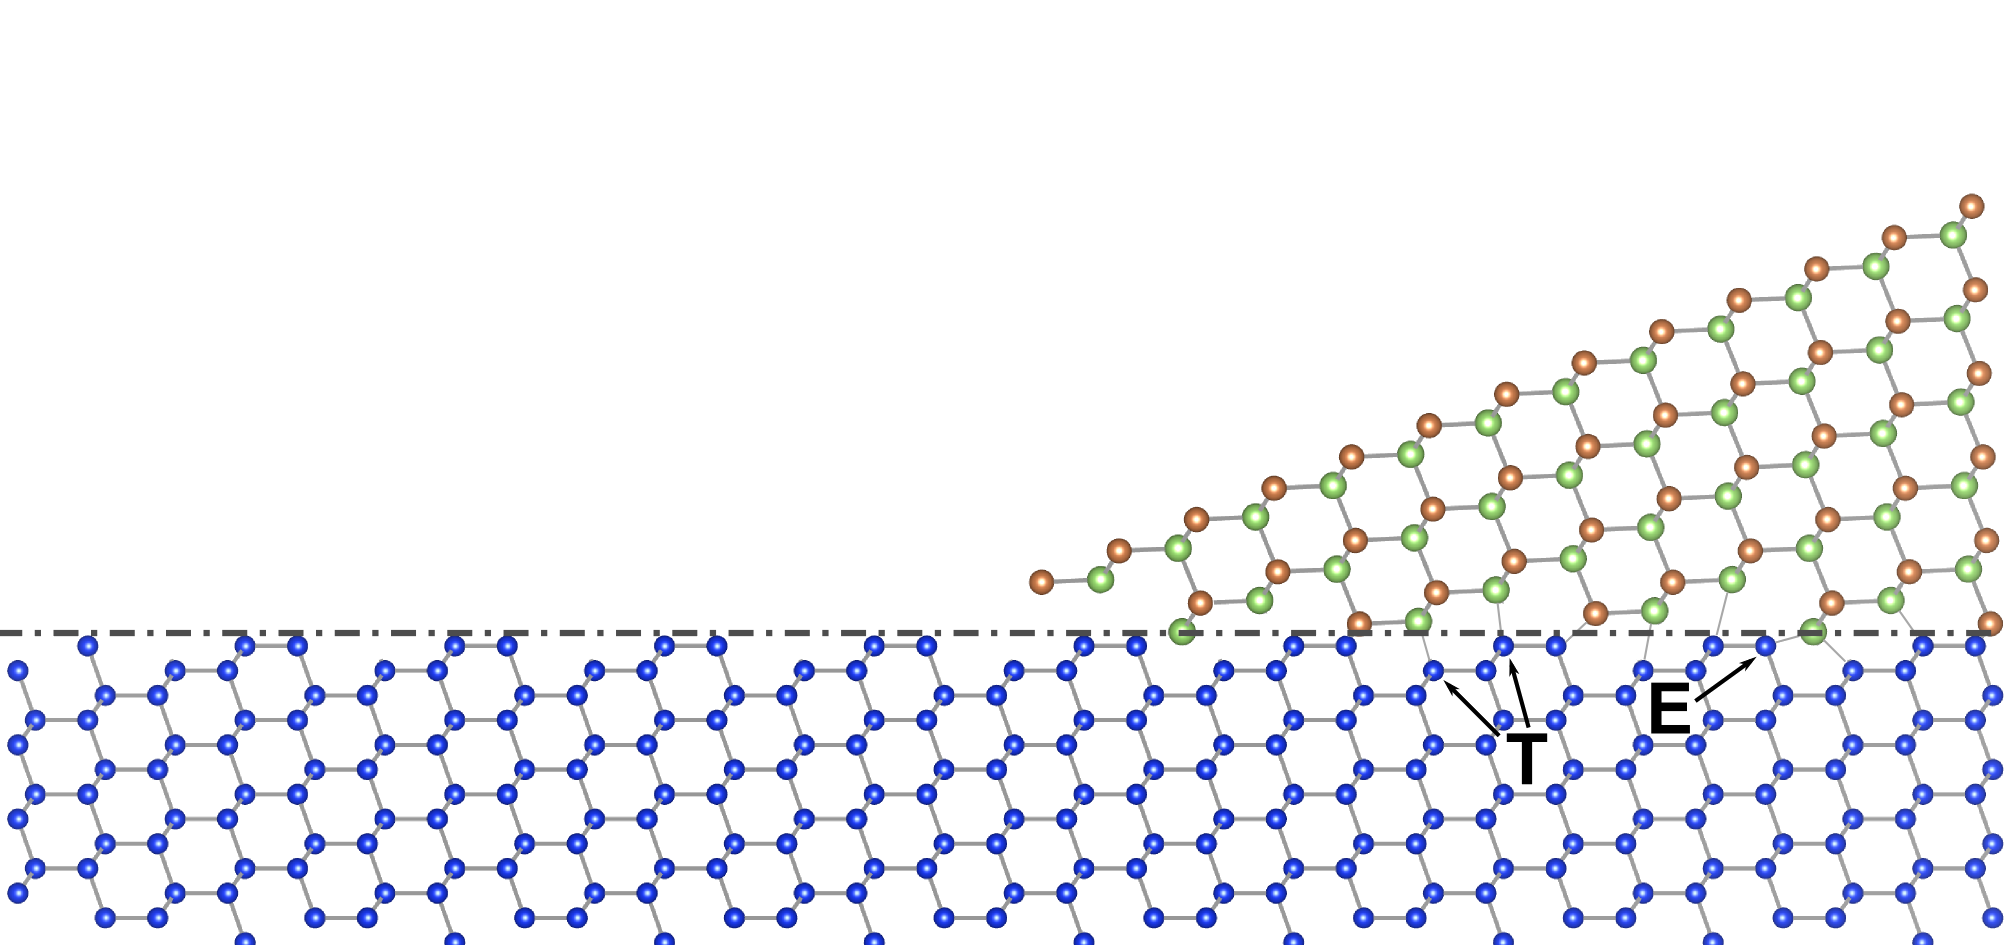
\includegraphics[width=\textwidth]{graphics/211_epi}
        \end{figure}}
                \only<3>{\begin{figure}
                        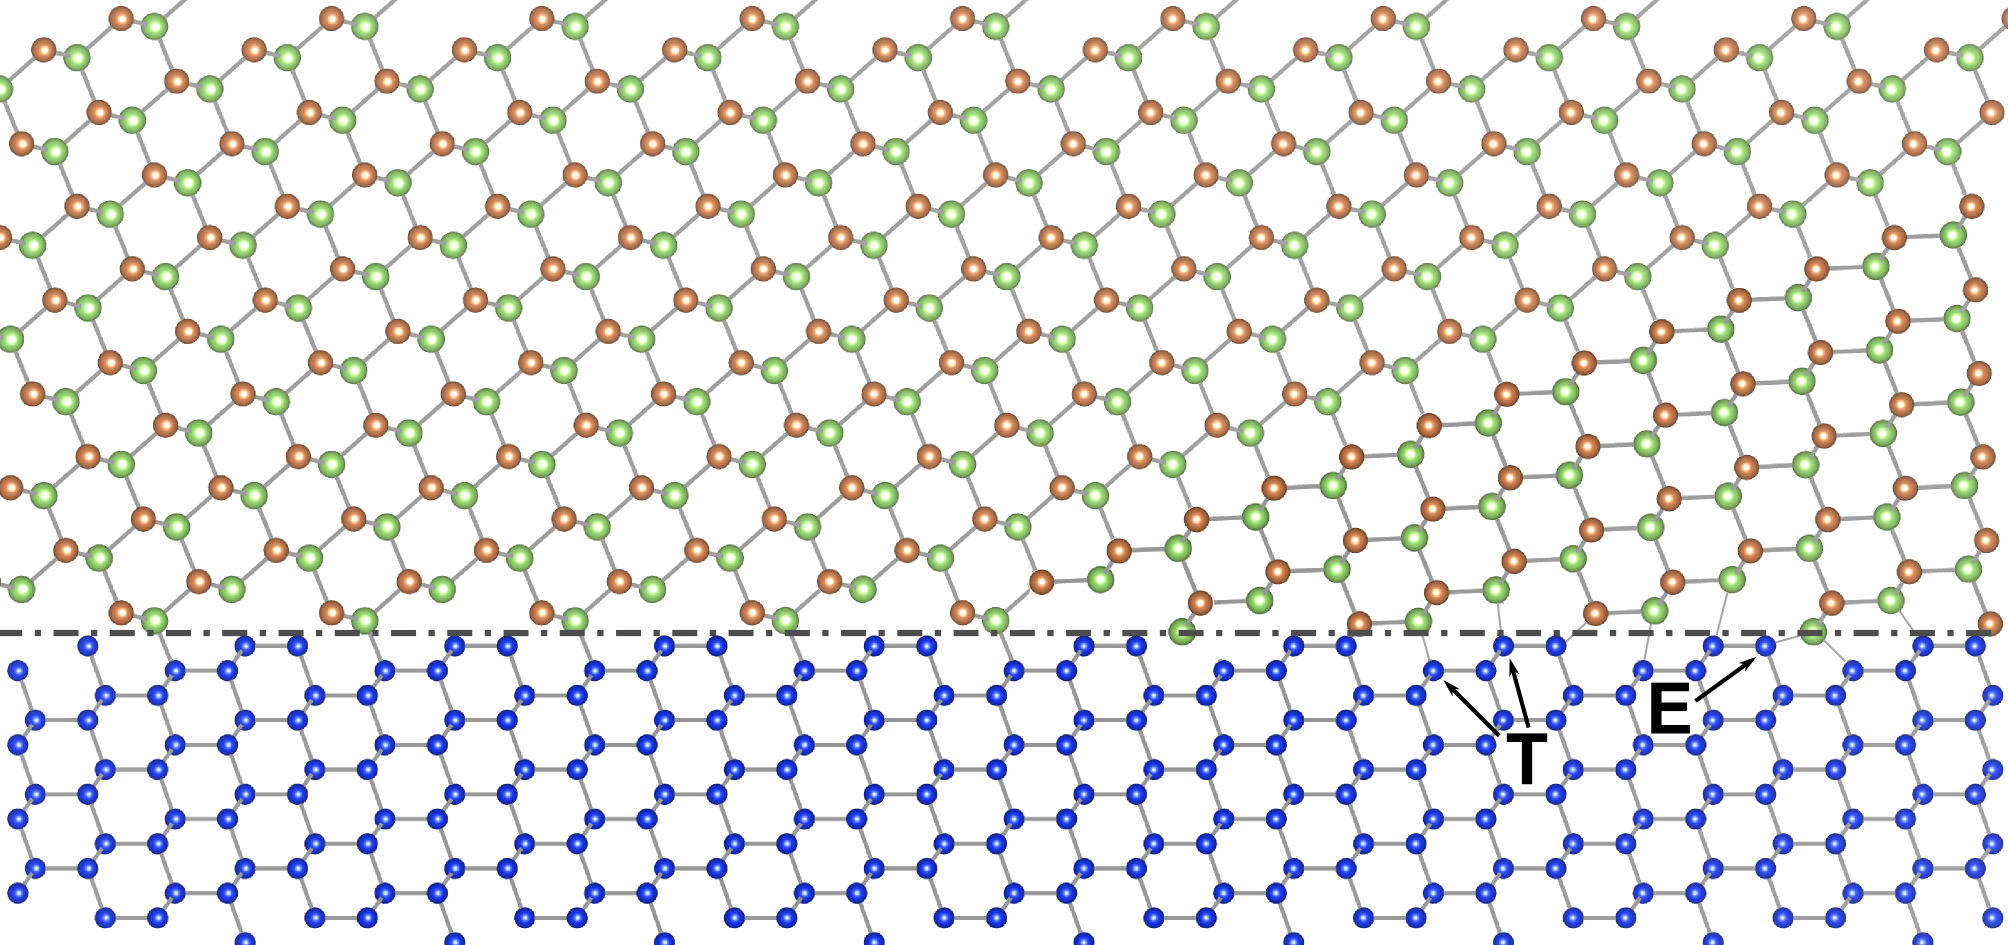
\includegraphics[width=\textwidth]{graphics/211_twin}
                    \end{figure}}
            \only<4>{\begin{figure}
                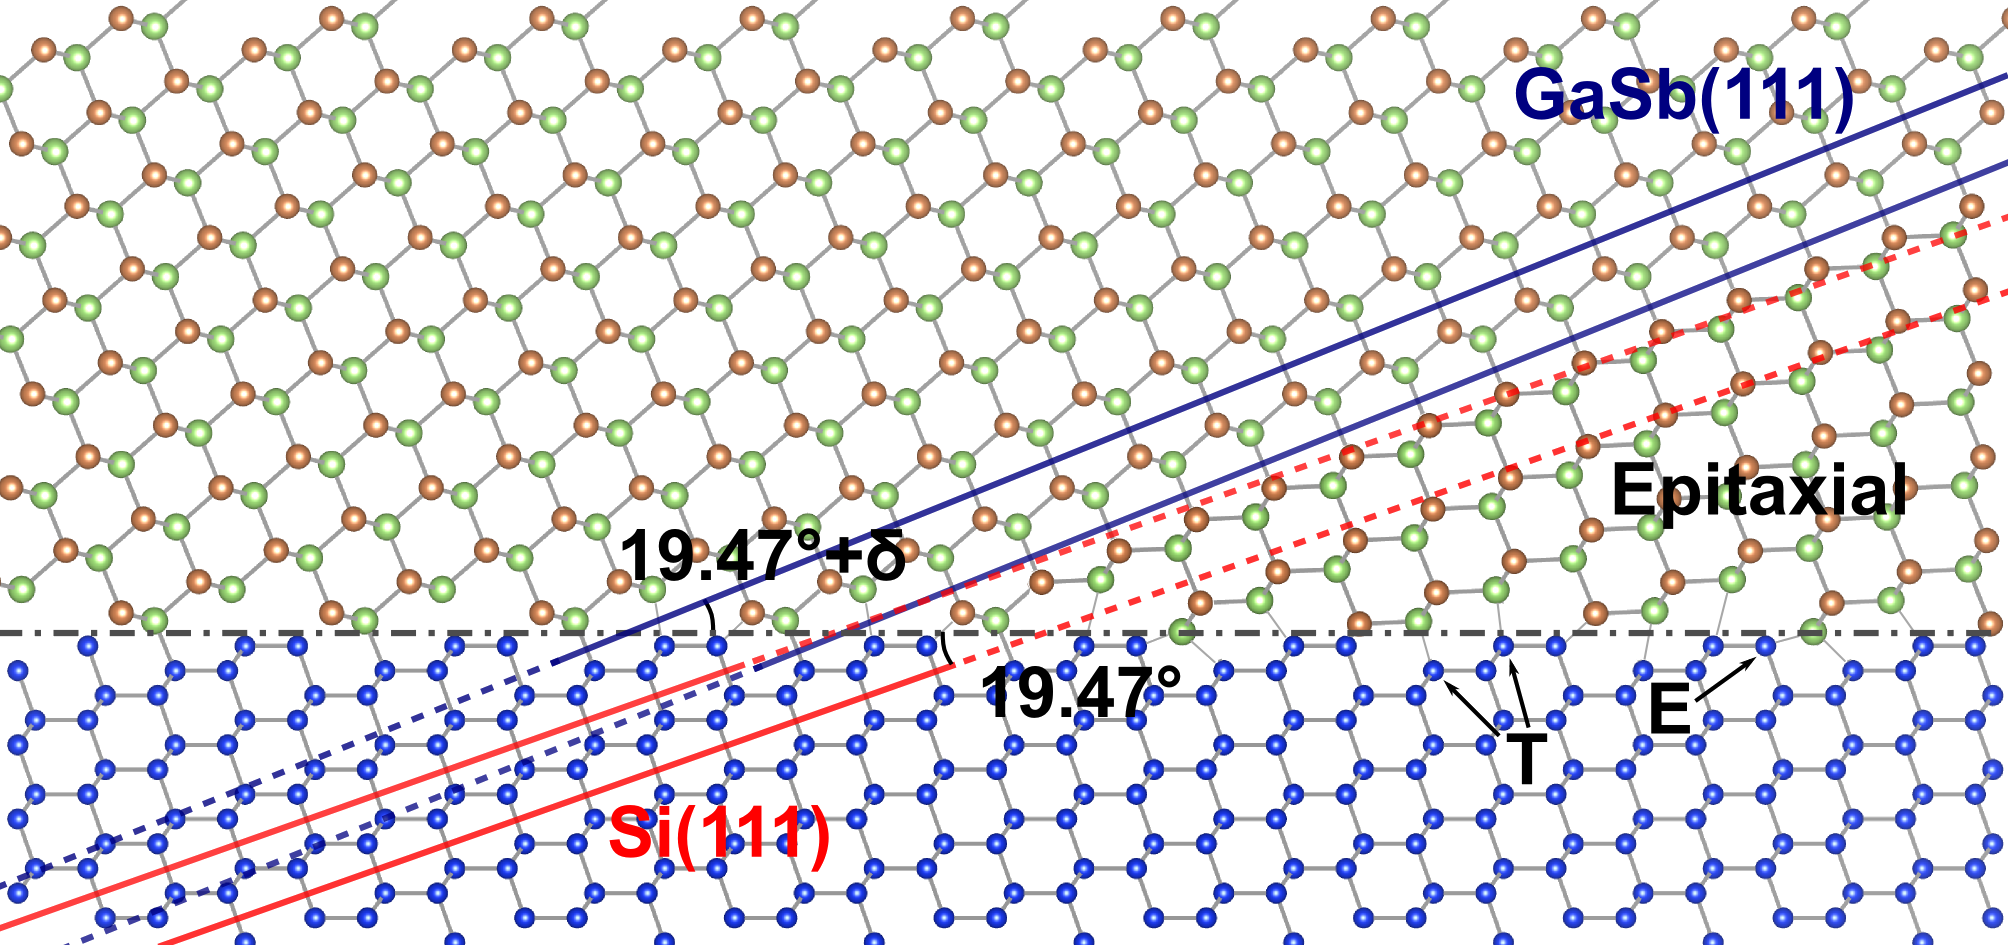
\includegraphics[width=\textwidth]{graphics/211_atoms_lines}
            \end{figure}}
    \only<5->{\begin{figure}
        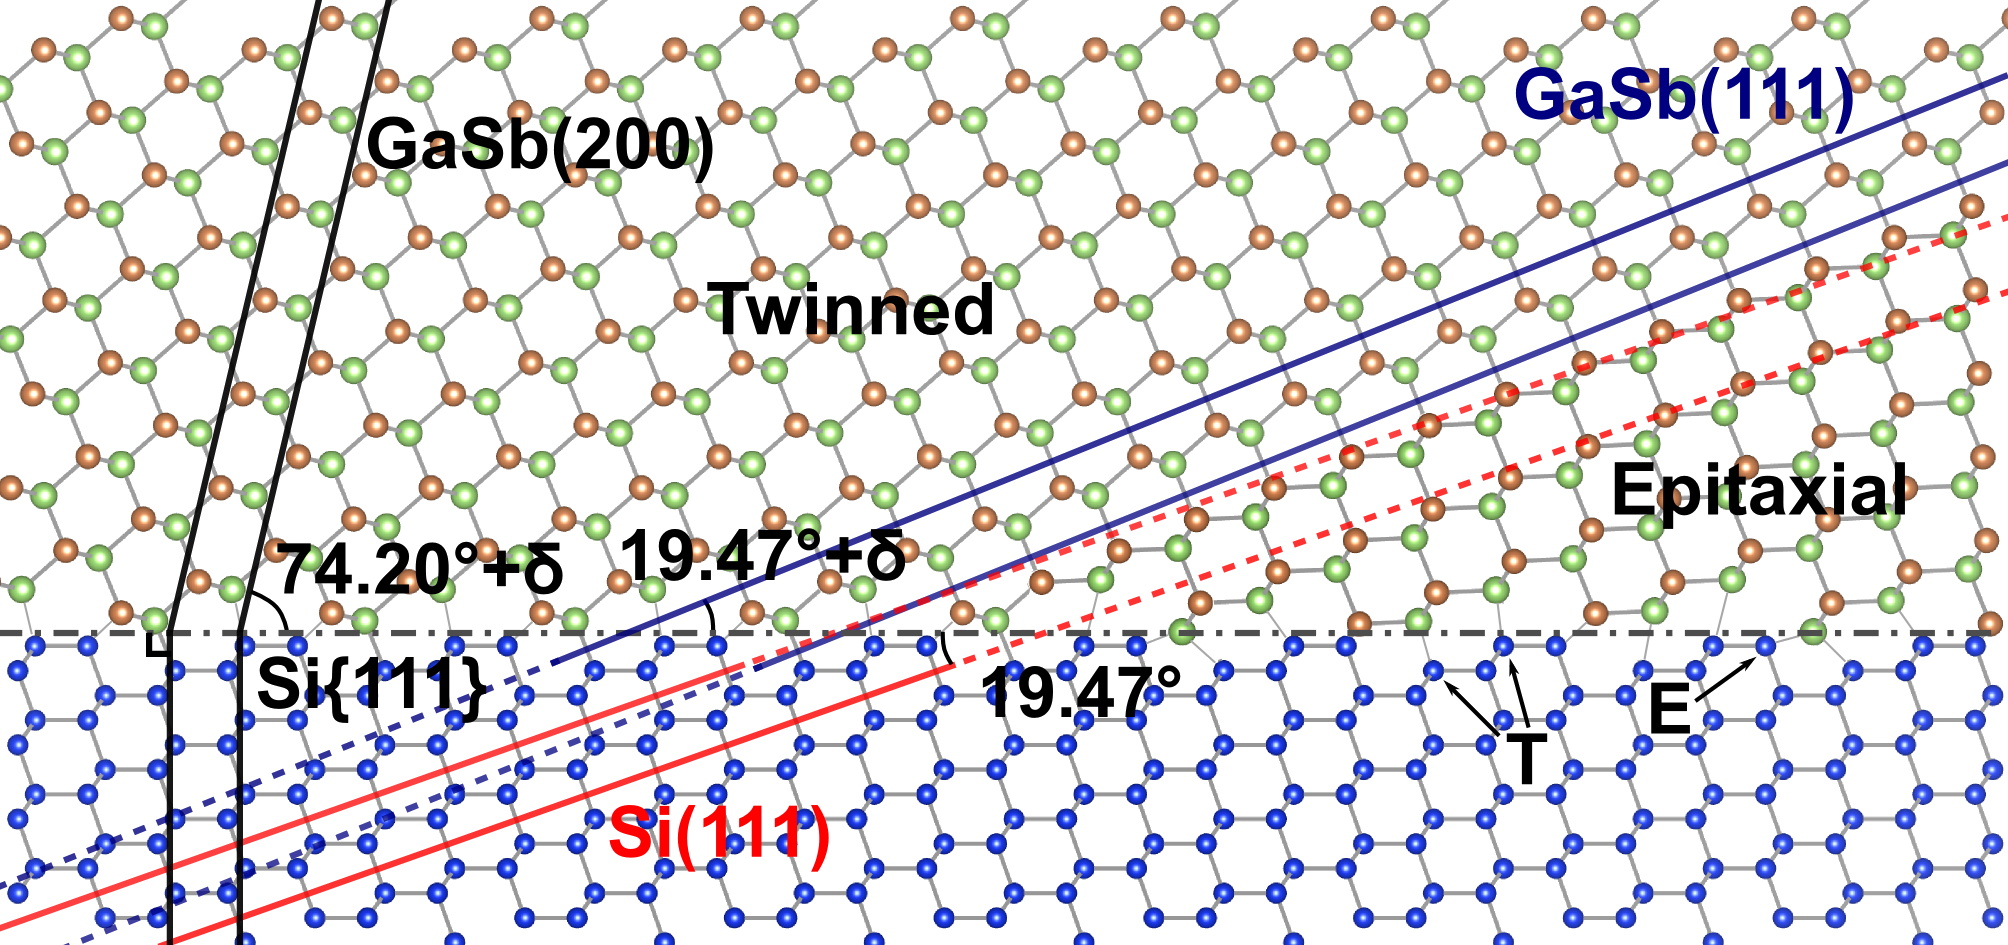
\includegraphics[width=\textwidth]{graphics/211_atoms_labelled}
    \end{figure}}
    \visible<4->{\begin{align*}
    \frac{ a_{GaSb}}{\sqrt{3} \sin(19.471^\circ + 2.5^{\circ})} \simeq \frac{a_{Si}}{\sqrt{3}\sin(19.471^\circ)}
    \end{align*}}
\end{frame}

\begin{frame}
    \begin{columns}[c]
        \begin{column}{0.41\textwidth}
            \begin{block}{Generalizing the Toy Model}
                \begin{itemize}[<+-| alert@+>]
                    \item Equate d-spacing of Silicon with projected d-spacing of GaSb
                    \item Generalize for any film and substrate combination
                    \item Strain for an arbitrary tilt is the difference between two plane spacing
                \end{itemize}
            \end{block}
        \end{column}
        \begin{column}{0.57\textwidth}
            \visible<1->{
                \begin{align*}
                \frac{ a_{GaSb}}{\sqrt{3} \sin(19.471^\circ + 2.5^{\circ})} \simeq \frac{a_{Si}}{\sqrt{3}\sin(19.471^\circ)}
                \end{align*}}
            \visible<2->{
                \begin{align*}
                \frac{ a_{film}}{\sqrt{3} \sin(19.471^\circ + \delta)} \simeq \frac{a_{sub}}{\sqrt{3}\sin(19.471^\circ)}
                \end{align*}}
            \visible<3->{
                \begin{align*}
                \varepsilon = \frac{ a_{film}}{\sqrt{3} \sin(19.471^\circ + \delta)} 
                - \frac{a_{sub}}{\sqrt{3}\sin(19.471^\circ)}
                \end{align*}
            }
        \end{column}
    \end{columns}
\end{frame}


\begin{frame}
    \begin{center}
        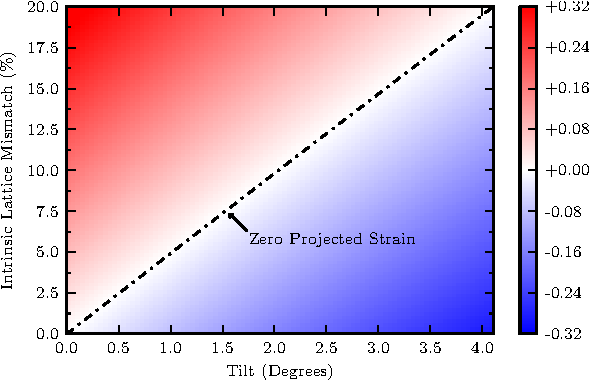
\includegraphics[width=0.95\textwidth]{graphics/tiltmap/step1}
    \end{center}
\end{frame}

\begin{frame}
    \begin{center}
        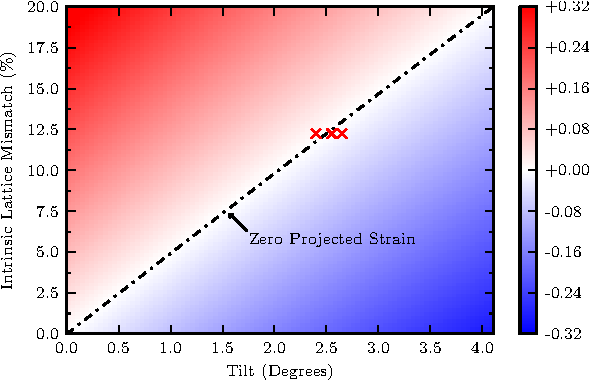
\includegraphics[width=0.95\textwidth]{graphics/tiltmap/step2}
    \end{center}
\end{frame}

\begin{frame}
    \begin{center}
        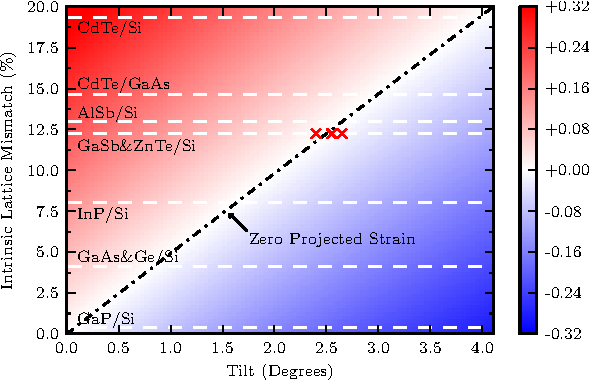
\includegraphics[width=0.95\textwidth]{graphics/tiltmap/step3}
    \end{center}
\end{frame}

\begin{frame}
    \begin{center}
        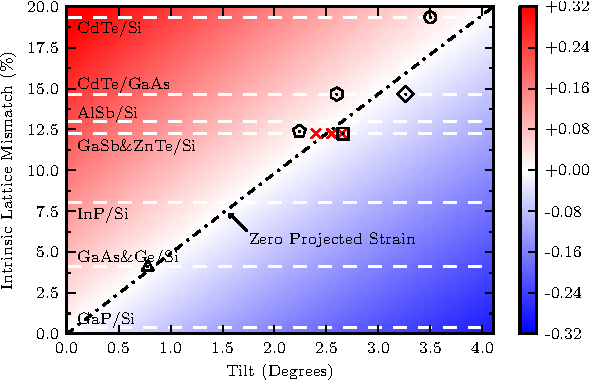
\includegraphics[width=0.95\textwidth]{graphics/tiltmap/step4}
    \end{center}
\end{frame}

\begin{frame}
    \frametitle{Epitaxy on (211) Silicon}
    \begin{block}{Conclusions}
        \begin{itemize}[<+-| alert@+>]
            \item The natural asymmetry of (211) allows the accommodation of strain  by tilting on an axis perpendicular to the asymmetry
            \item Tilt is driven by the alignment of (111) planes between the substrate and the thin film
            \item Tilt allows strain accommodation over a lattice mismatch of 0-20\%
        \end{itemize}
    \end{block}
\end{frame}

\section{Unusal Bond Energies at Interfaces}
\subsection{CdTe on Sapphire Epitaxy and Liftoff}
\begin{frame}
    \frametitle{Outline}
    \tableofcontents[currentsection,currentsubsection]
\end{frame}
\begin{frame}
    \frametitle{Introduction}
    \begin{columns}
        \begin{column}{0.5\textwidth}
            \begin{block}{Unusual Bond Energies}
                \begin{itemize}[<+-| alert@+>]
            \item Typically, epitaxial bonds are covalent or ``chemisorbed'' in strength
            \item Interface energies are comparable to in-bulk energies
            \item Bond energies between chemically dissimilar materials are very different
            \item Bond energy differences have implications for strain, post-treatment of films and defect formation
                \end{itemize}
            \end{block}
        \end{column}
        \begin{column}{0.5\textwidth}
            \centering
            \visible<1->{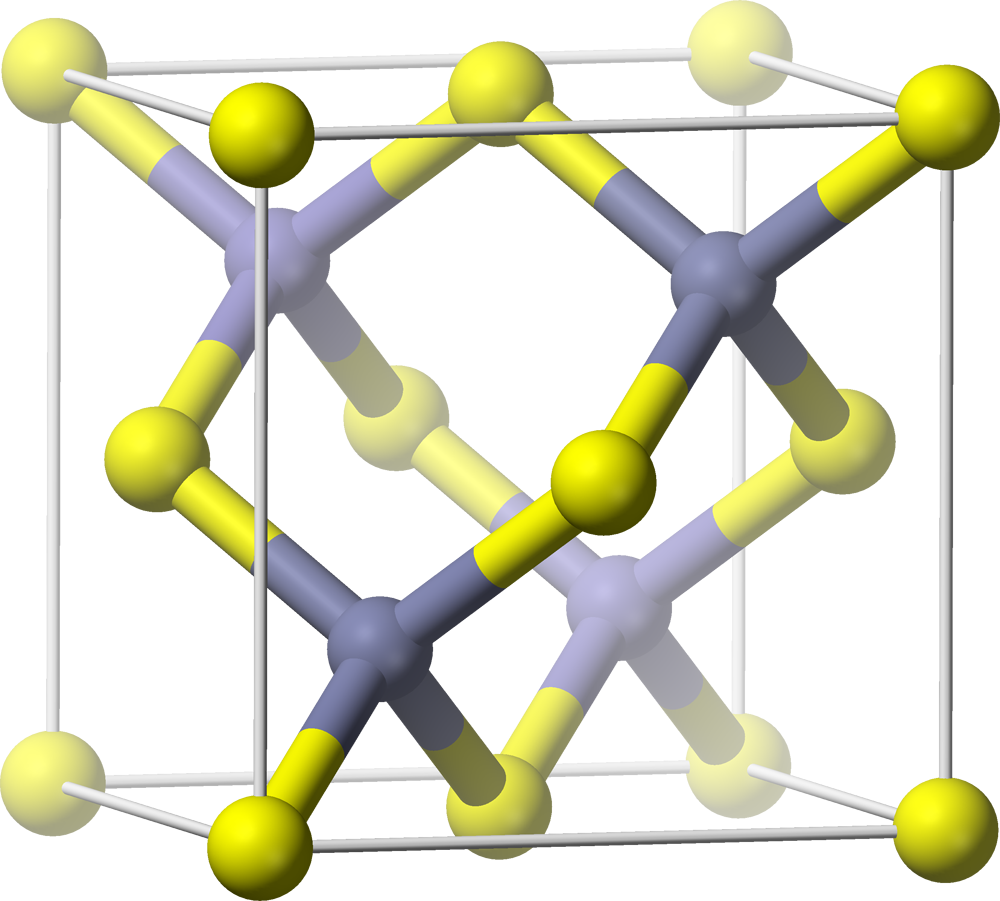
\includegraphics[height=0.4\textheight]{graphics/zincblende}\\ \TINY Wikipedia: Zincblende} \\
            \visible<3->{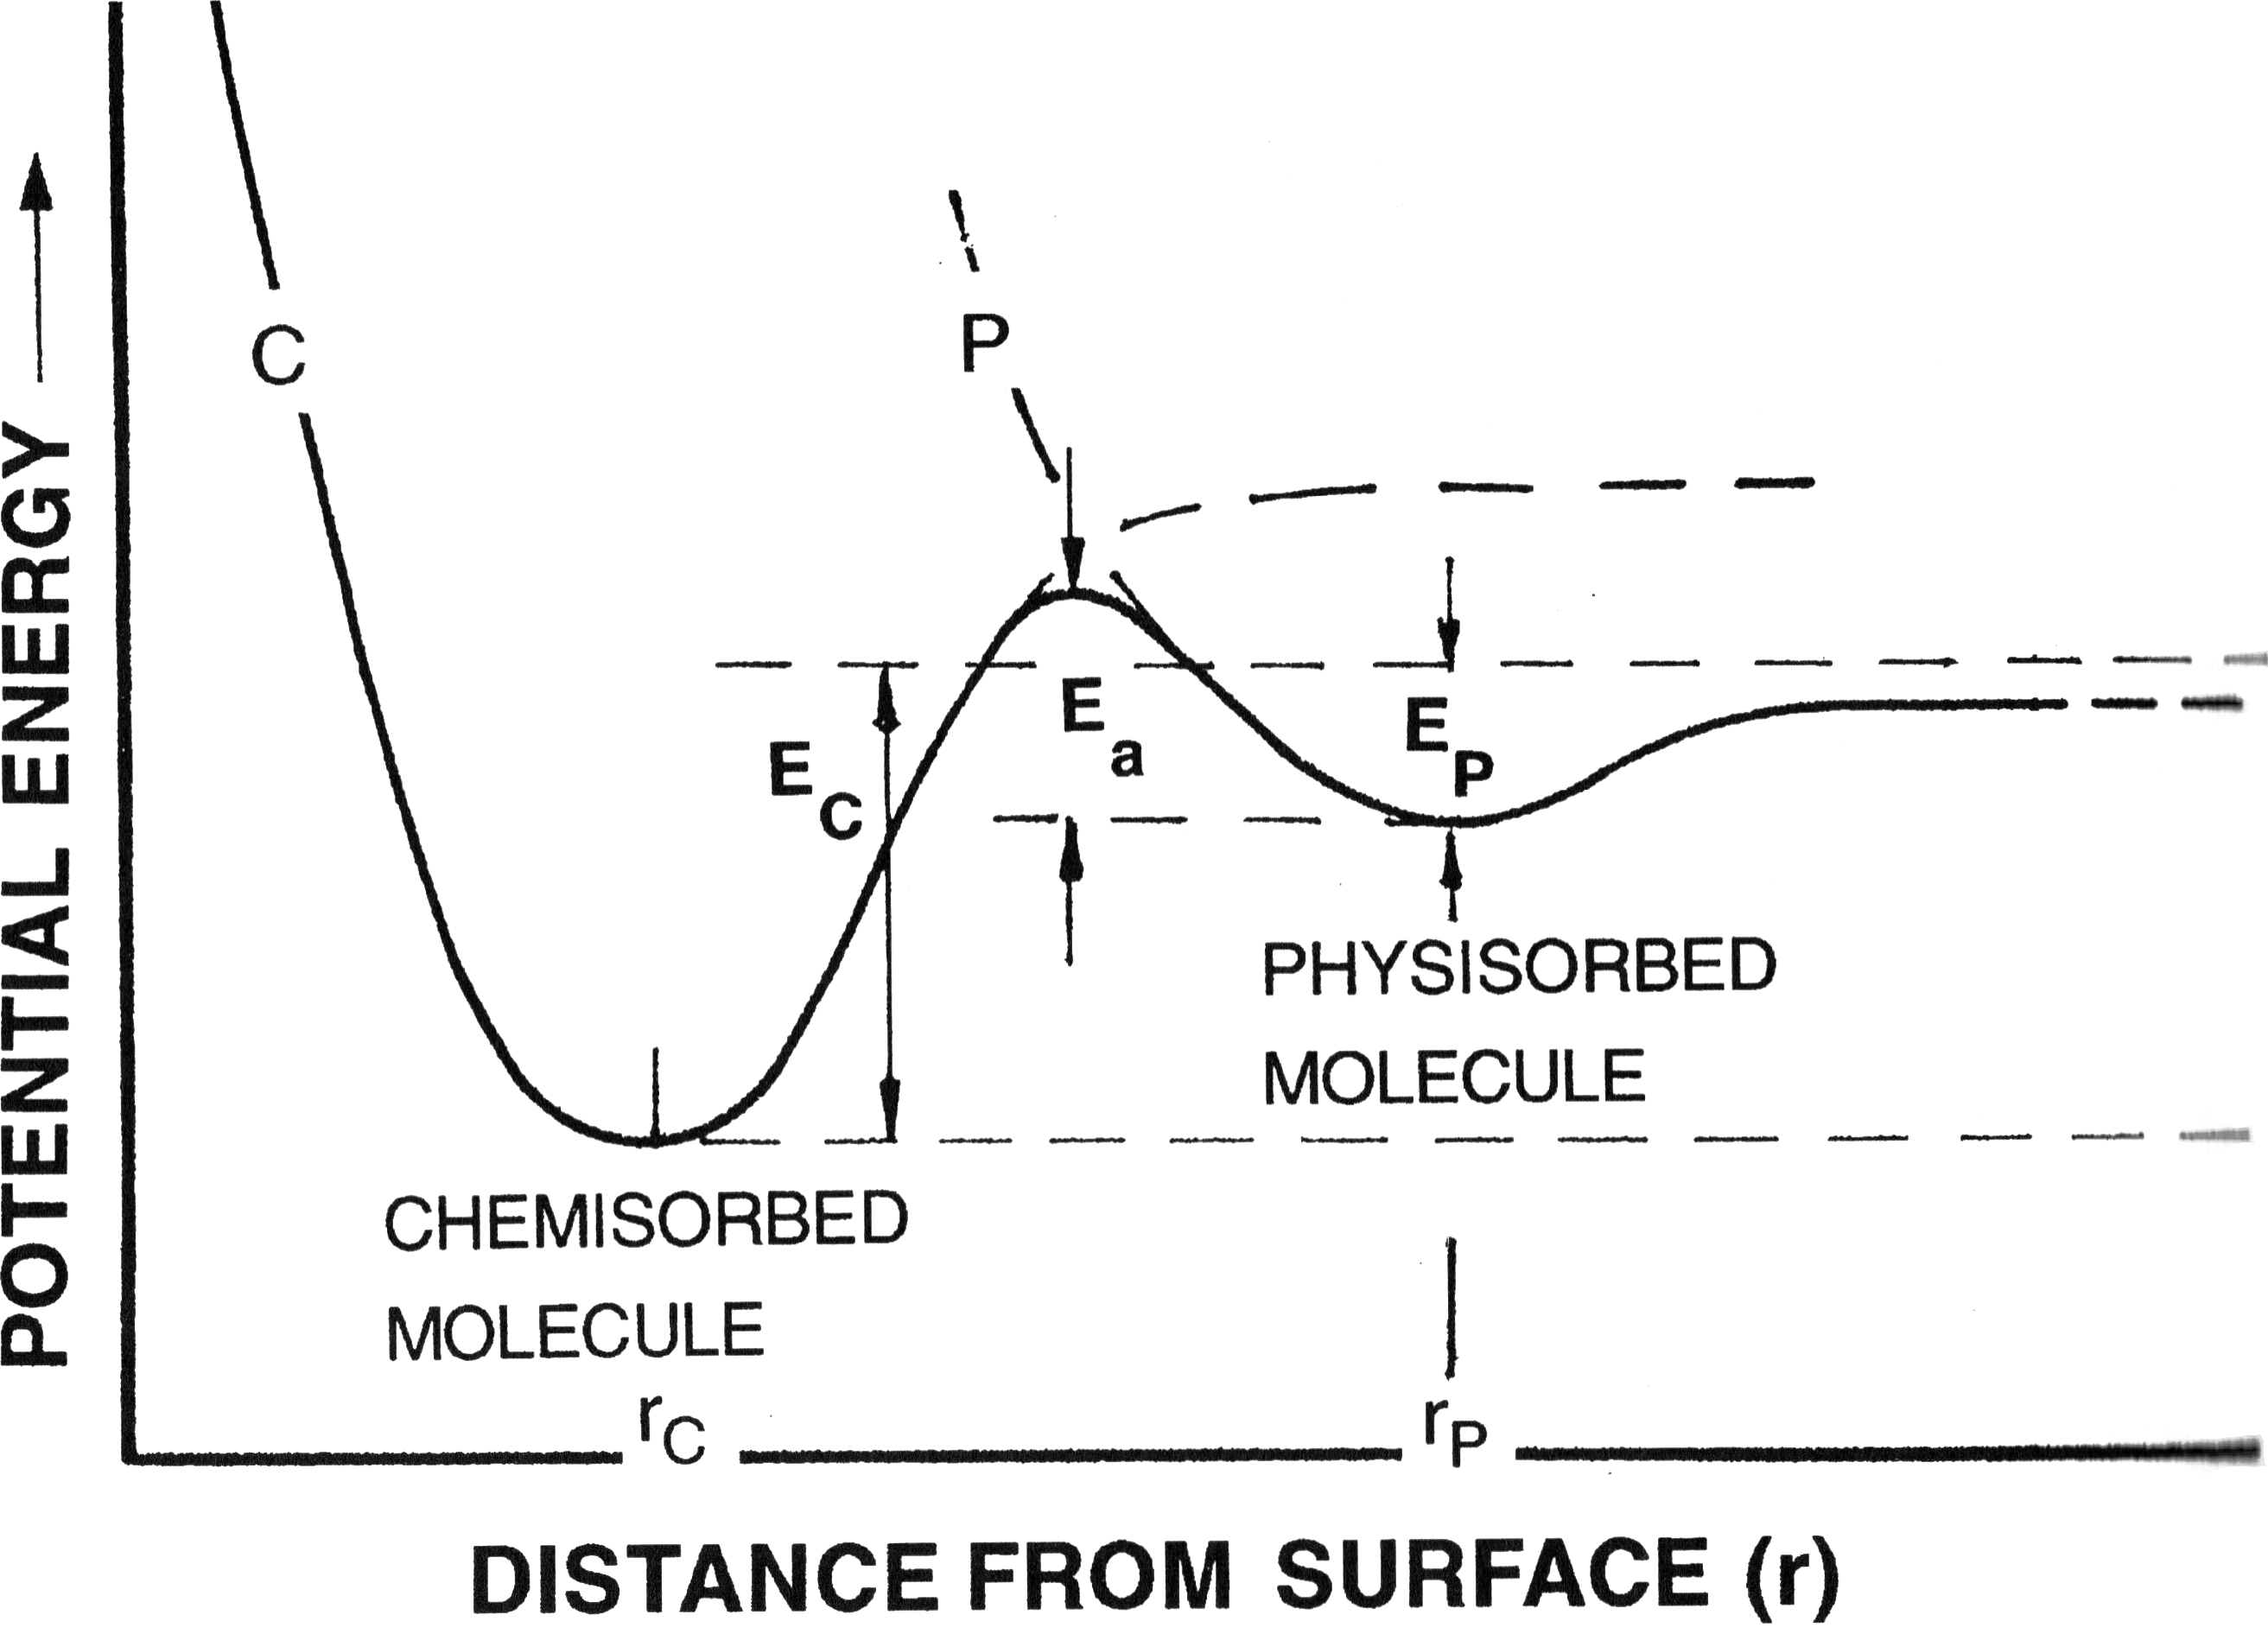
\includegraphics[height=0.45\textheight]{graphics/back_bond_potential} \\ \TINY M. Ohring, Materials Science of Thin Films, 2nd ed. San Diego: Elsevier Science, 2001.}
        \end{column}
    \end{columns}
\end{frame}

\begin{frame}
    \frametitle{Experimental}
    \begin{columns}
        \begin{column}{0.5\textwidth}
            \begin{block}{Unusual Bond Energies}
                \begin{itemize}[<+-| alert@+>]
                    \item Growth of CdTe thin films and nanowires has been highly successful on sapphire via PLD
                    \item Nanowire adhesion appeared to be oddly weak despite epitaxial alignment
                    \item How did these nanowires stay in place?
                    \item Similar issues arose when applying contacts for electrical measurements
                \end{itemize}
            \end{block}
        \end{column}
        \begin{column}{0.5\textwidth}
            \centering
            \only<1>{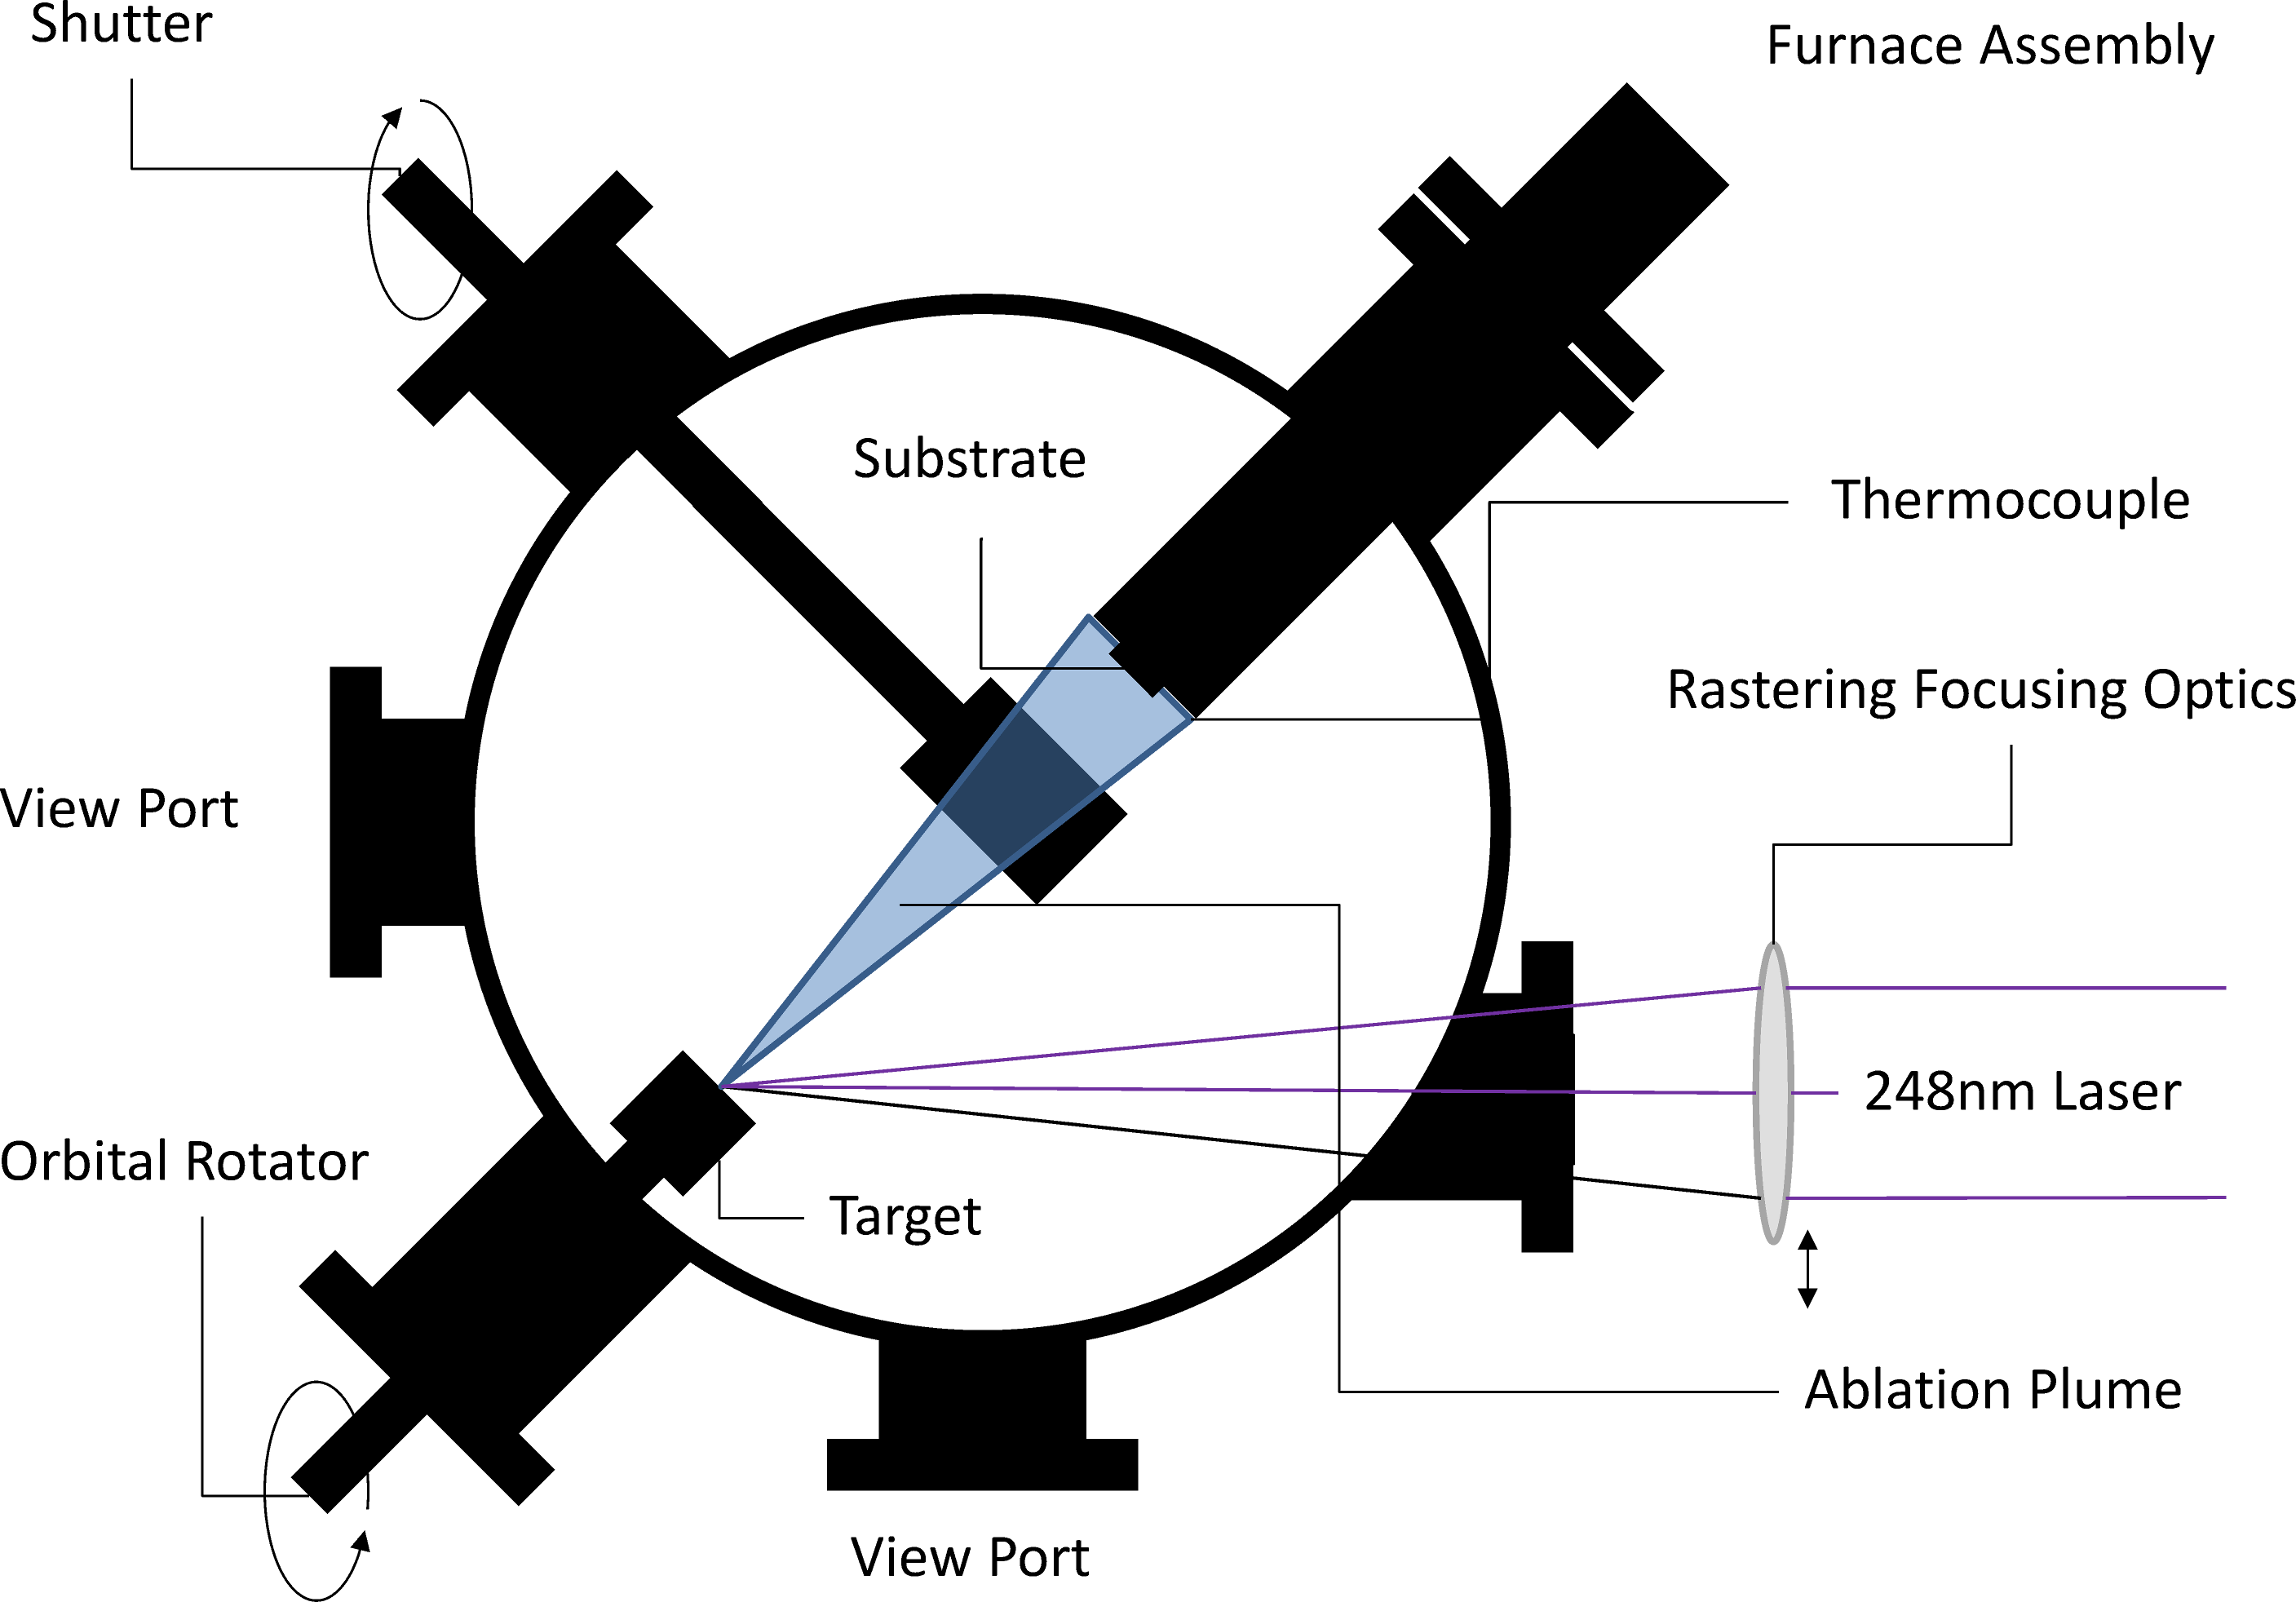
\includegraphics[width=\textwidth]{graphics/exp_PLD_chamber}} \\
            \only<2->{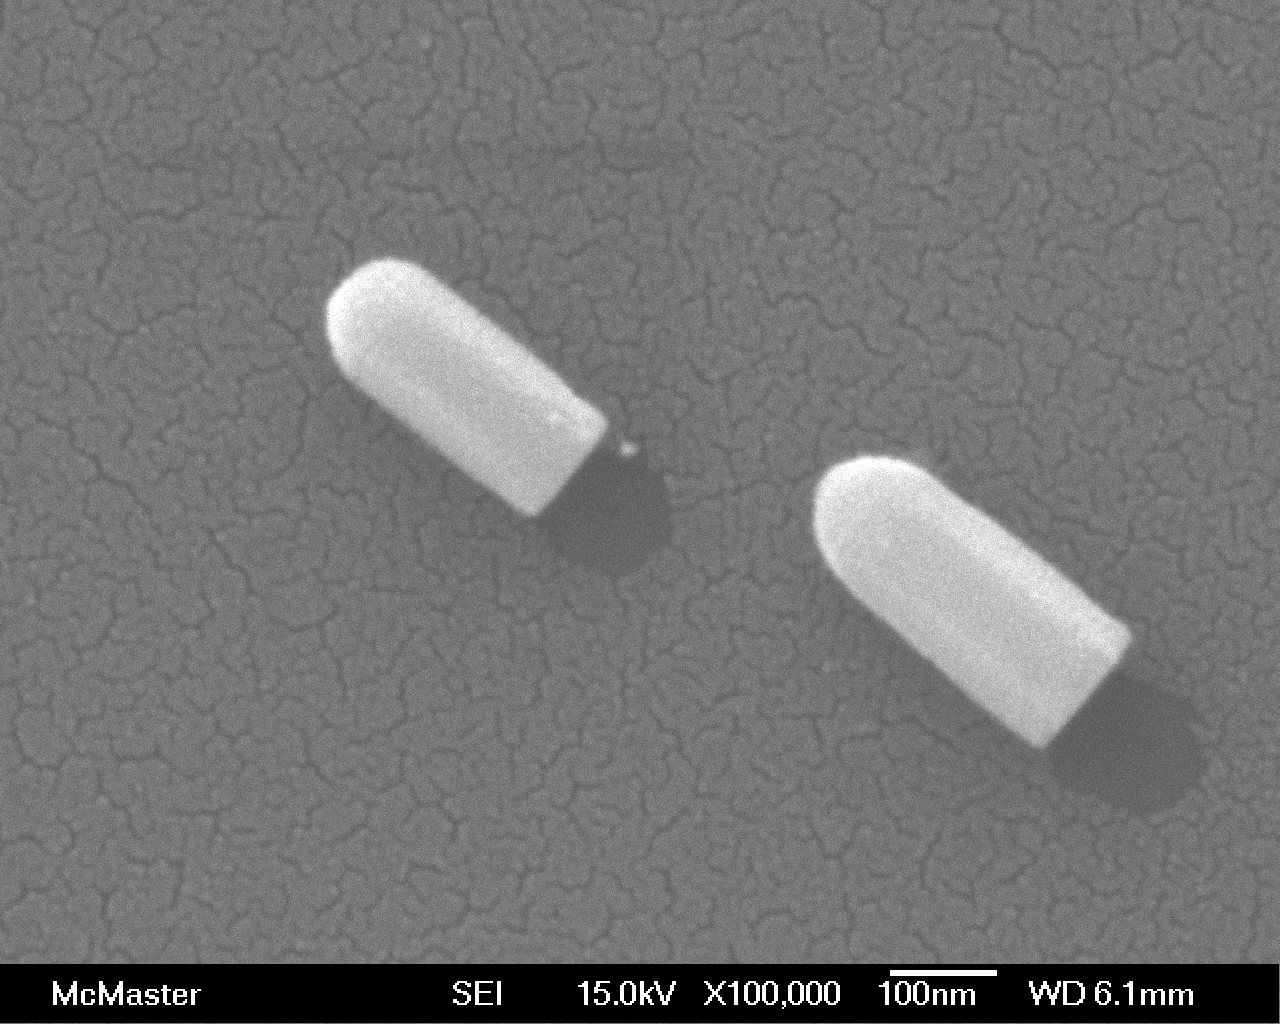
\includegraphics[width=\textwidth]{graphics/cdteliftoff_nanowires}}
        \end{column}
    \end{columns}
\end{frame}


\begin{frame}
\frametitle{The Process}
    \begin{center}
    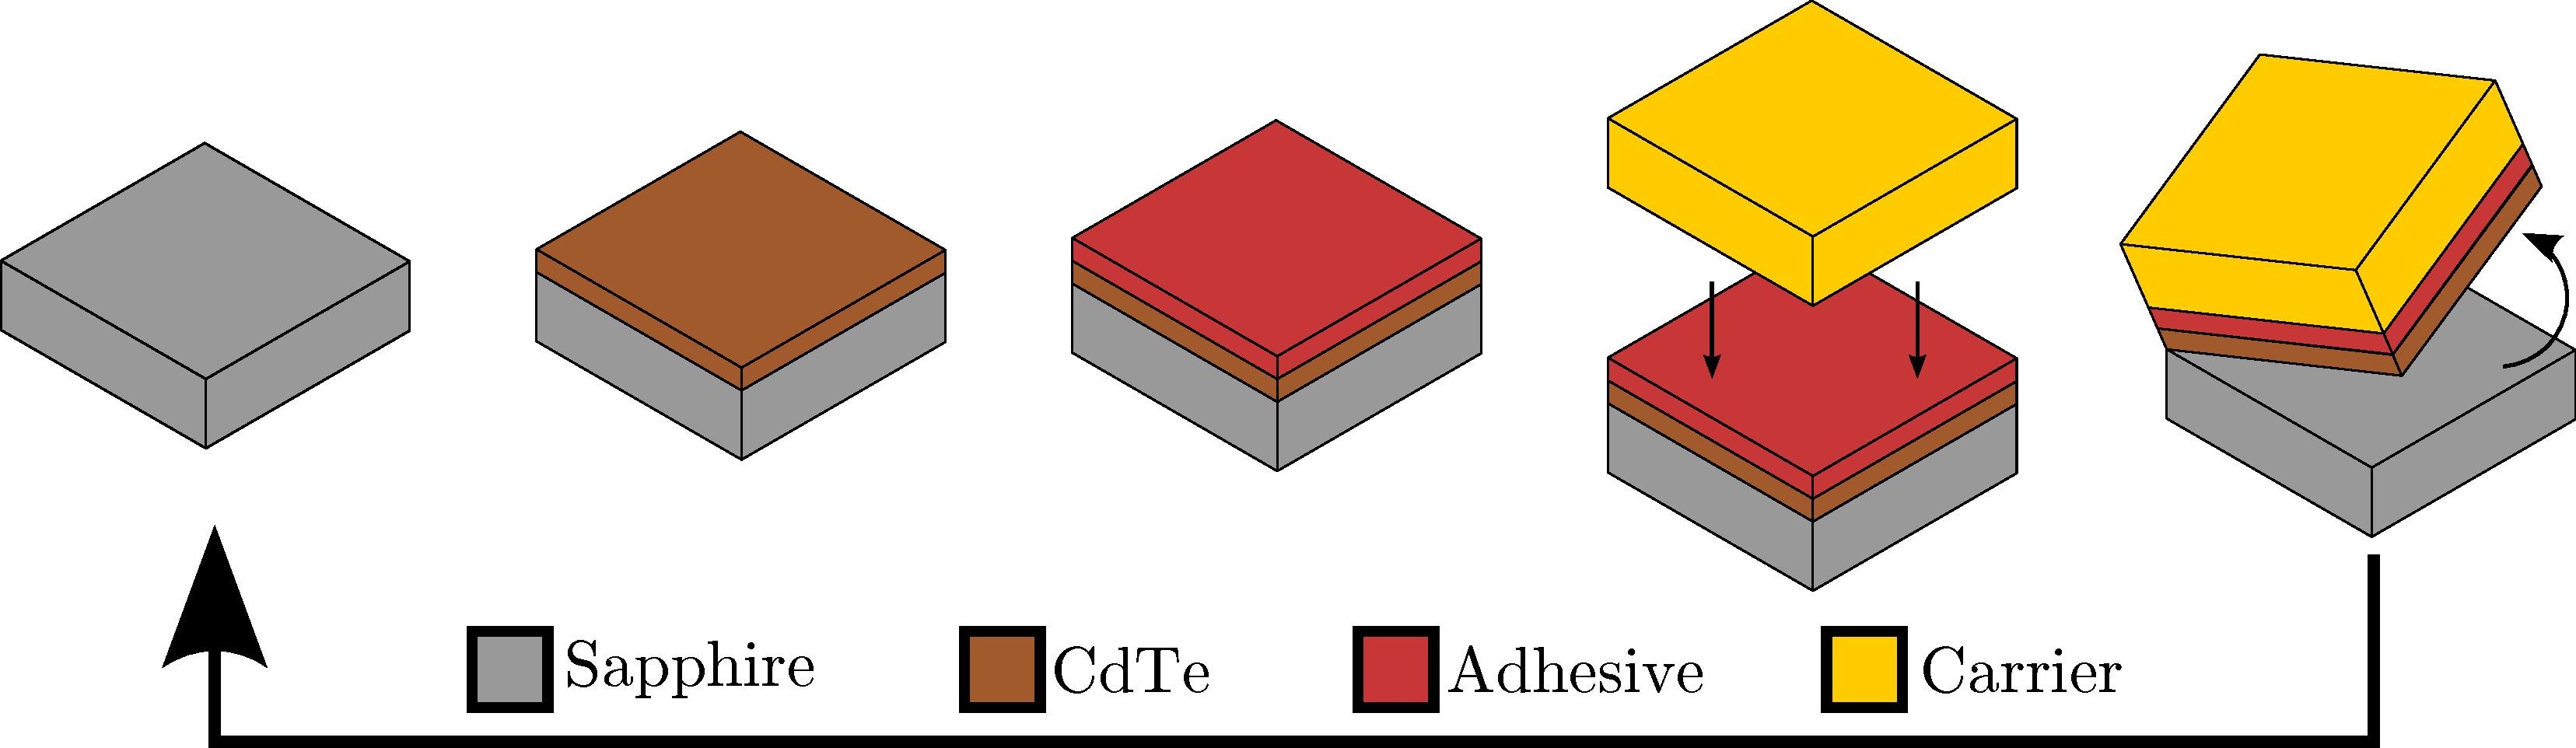
\includegraphics[width=\textwidth,height=0.9\textheight,keepaspectratio]{graphics/cdteliftoff_process}
    \end{center}
\end{frame}

\begin{frame}
    \frametitle{Practical Results}
    \begin{columns}
        \begin{column}{0.5\textwidth}
            \centering
            \includegraphics[width=0.8\textwidth]{graphics/cdteliftoff_liftoff} \\
            CdTe on Optical Adhesive Carrier
        \end{column}
        \begin{column}{0.5\textwidth}
            \centering
            \includegraphics[width=0.8\textwidth]{graphics/cdteliftoff_sapphire} \\
            (Mostly) Clean Sapphire Substrate
        \end{column}
    \end{columns}
\end{frame}

\begin{frame}
    \frametitle{2DXRD Results}
    \begin{columns}
        \begin{column}{0.5\textwidth}
            \centering
            \includegraphics[width=0.9\textwidth]{graphics/cdteliftoff_F22_attached} \\
            CdTe on Sapphire (111) Pole Figure
        \end{column}
        \begin{column}{0.5\textwidth}
            \centering
            \includegraphics[width=0.9\textwidth]{graphics/cdteliftoff_F22_released} \\
            CdTe Liftoff on Epoxy Carrier
        \end{column}
    \end{columns}
\end{frame}



\begin{frame}
    \begin{columns}
\begin{column}{0.5\textwidth}
    \begin{block}{Results}
        \begin{itemize}[<+-| alert@+>]
            \item Liftoff process is near 100\% effective, subject to better processing
            \item Liftoff is not destructive to crystal structure
            \item Liftoff relieves strain in CdTe, improving X-ray peak widths
            \item Leftover sapphire substrate is suitable for CdTe growths (after cleaning)
        \end{itemize}
    \end{block}
\end{column}
\begin{column}{0.5\textwidth}
    \centering
    \visible<1->{\includegraphics[width=0.65\textwidth]{graphics/cdteliftoff_liftoff}} \\ \vspace{0.25cm}
    \visible<2->{\includegraphics[width=0.65\textwidth]{graphics/liftoff_solder}}
\end{column}
        \end{columns}
\end{frame}

\section{Conclusions}
\begin{frame}
    \begin{block}{Results and Conclusions}
        \begin{itemize}[<+-| alert@+>]
            \item Symmetry and Symmetry Breaking
            \begin{itemize}
                \item Vicinal substrates influence thin film growth through asymmetric enhancements of growth rate
                \item Naturally asymmetric surfaces allow for strain accommodation through tilt during epitaxy
            \end{itemize}
            \item Unusal Bond Energies at Interfaces
                        \begin{itemize}
                            \item Chemically dissimilar epitaxy results in a new phenomenon of liftoff with potential engineering applications
                        \end{itemize}
        \end{itemize}
    \end{block}
\end{frame}

\begin{frame}
    \begin{center}
            \Huge Thank You
    \end{center}

\end{frame}

\appendix

\begin{frame}
   \includegraphics[width=\textwidth]{graphics/intro_bandgaps}
\end{frame}

\begin{frame}
    \begin{columns}
        \begin{column}{0.5\textwidth}
            \centering
            \includegraphics[width=\textwidth]{graphics/mbeoxide_InSbSaph2} \\ InSb on Sapphire
        \end{column}
        \begin{column}{0.5\textwidth}
            \centering
            \includegraphics[width=\textwidth]{graphics/mbeoxide_InSbSpaph2liftoff} \\ InSb on Epoxy Carrier
        \end{column}
    \end{columns}
\end{frame}

\begin{frame}
    \frametitle{Low Temperature Photoluminesnce}
    \begin{center}
        \includegraphics[width=\textwidth]{graphics/cdteliftoff_PL_attached}
    \end{center}
\end{frame}

\begin{frame}
        \frametitle{Low Temperature Photoluminesnce}
    \begin{center}
        \includegraphics[width=\textwidth]{graphics/cdteliftoff_PL_joined}
    \end{center}
\end{frame}

\end{document}
